%//------ Section 03 -------------------------------------------------------------------------------------------------
\chapter{Mass measurements of multi-strange baryons in pp collisions at \sqrtS = 13 TeV}
\label{chap:CPTAnalysis}
%//-----------------------------------------------------------------------//

The first analysis conducted in this thesis aims at measuring the masses and mass differences between particle and anti-particle of multi-strange baryons. The focus is on \rmXiM, \rmAxiP, \rmOmegaM and \rmAomegaP. This chapter provides a description of the different elements needed to achieve this goal. \\

Once the context has been introduced (\Sec\ref{sec:IntroductionCPT}), the exploited data samples are presented in \Sec\ref{sec:DataSampleCPT}. This is followed by a detailed description and discussion of the various ingredients involved in the analysis (\Sec\ref{sec:AnalysisOfHyperonMasses}): the track, V0 and cascade candidate selections, and finally, the principles of the mass measurement. By design, such a measurement depends on the different elements of the analysis. Therefore, each of them must be studied in order to identify those affecting the mass extraction and account it in the final results. This review of the analysis is at the heart of \Sec\ref{sec:SystStudy}. Finally, this chapter comes to an end with a summary of the different systematic biases and associated uncertainties, and a discussion of the final results in \Sec\ref{sec:FinalResultsCPT}. 

\section{Introduction}
\label{sec:IntroductionCPT}

%Symmetries certainly stand as one of the most fruitful concepts in Physics. They are of two kinds: continuous --- such as the global translations in both space and time, or the Lorentz transformations --- and discrete --- for example, the space- (P) and time- (T) inversions, the charge conjugation (C), and their combined transformation given by CPT. In particular, the Lorentz and CPT symmetries are connected by the so-called CPT theorem which states that any local Lorentz-invariant quantum field theory must also (under some extra requirements) be CPT invariant \cite{cptstatus}. Consequently, the CPT violation implies the breaking of the Lorentz symmetry, and vice versa\footnote{In fact, there is another option; to allow for CPT to be violated, either the Lorentz symmetry must be broken -- as in the string theory \cite{string} or the Standard-Model Extension \cite{sme} -- or some of the other extra assumptions of the CPT theorem must be dropped, namely the energy positivity, local interactions, finite spin, etc \cite{cptimplieslorentz}\cite{cptsymmetryantitsviolation}. } \cite{sozzi}. Another implication involves the relation between the properties of matter and antimatter: due to the charge conjugation linking particles to antiparticles, the CPT symmetry imposes that they share the same invariant mass, energy spectra, lifetime, coupling constants, etc \cite{cptsymmetryantitsviolation}. Most of the experimental checks of CPT invariance stem from these physical consequences.

As discussed in \Sec\ref{subsec:Theory}, the Standard Model is built upon a set of symmetries, each being either discrete -- such as the combination of the charge conjugation (C), parity (P) and time reversal (T), known as the CPT transformation -- or continuous -- for example, the Lorentz transformations that includes rotations and boosts. In particular, the Lorentz and CPT symmetries are connected by the so-called CPT theorem which establishes that any unitary, local Lorentz-invariant quantum field theory must be CPT invariant \cite{kosteleckyStatusCPT1998}. Consequently, the CPT violation implies the breaking of the Lorentz symmetry, and vice versa\footnote{In fact, another option exists; to allow for the CPT violation, either the Lorentz symmetry must be broken -- as in the case of string theory \cite{kosteleckySpontaneousBreakingLorentz1989} or the Standard-Model Extension \cite{colladayLorentzviolatingExtensionStandard1998} -- or some of the other additionnal assumptions of the CPT theorem must be dropped, namely the energy positivity \cite{abersDiseasesInfiniteComponentField1967}, local interactions \cite{carruthersIsospinSymmetryTCP1968}, finite spin \cite{oksakInvalidityTCPtheoremInfinitecomponent1968}, etc \cite{lehnertCPTSymmetryIts2016}\cite{greenbergCPTViolationImplies2002}. } \cite{sozziTestsDiscreteSymmetries2019}. Another implication involves the relation between the properties of matter and antimatter: due to the charge conjugation linking particles to antiparticles, the CPT symmetry imposes that they share the same invariant mass, energy spectra, lifetime, coupling constants, etc \cite{lehnertCPTSymmetryIts2016}. Most of the experimental checks of CPT invariance stem from this last point, which imposes several constraints on the anti-particle properties. \\

The Particle Data Group (PDG) \cite{particledatagroupReviewParticlePhysics2022} compiles a large variety of CPT tests from many experiments and with different degrees of precision; so far, no CPT violation has been observed. The most stringent test involves the \rmKzero-\rmAKzero mixing process, which depends on the mass and lifetime differences of these two states. In this way, assuming no other source of CPT violation in the decay of neutral kaons, these two quantities have been bounded \cite{particledatagroupReviewParticlePhysics2022}\cite{angelopoulosK0OverlineK1999} to 

\begin{equation}
2 \frac{\mid m_{\rmKzero} - m_{\rmAKzero} \mid}{m_{\rmKzero} + m_{\rmAKzero}} < 6 \times 10^{-19} \quad , \quad 2 \frac{\mid \Gamma_{\rmKzero} - \Gamma_{\rmAKzero} \mid}{\Gamma_{\rmKzero} + \Gamma_{\rmAKzero}} = (8 \pm 8) \times 10^{-18}.
\end{equation}

These indirect limits are much stronger than the ones extracted from direct tests. For example, in the hyperon sector, the precision on relative mass difference is typically of a few $10^{-5}$. In the latter case, it should be mentioned that there is still some room for improvements, and most particularly concerning the mass difference measurements between particle and anti-particle in the multi-strange baryon sector. The only test of this kind dates back to 2006 \cite{abdallahMassesLifetimesProduction2006} for the \rmXiM and \rmAxiP, and from 1998 \cite{chanMeasurementPropertiesOverline1998} for the \rmOmegaM and \rmAomegaP. The former was achieved by exploiting 3.25 million hadronic decays of the \rmZzero recorded by the DELPHI detector at LEP-1; the latter was obtained on the E756 spectrometer at Fermilab, using an 800-\gmom proton beam on a beryllium target. However, both studies suffer from low statistics: approximately 2500(2300) reconstructed \rmXiM (\rmAxiP) and about 6323(2607) reconstructed \rmOmegaM (\rmAomegaP) were used.\\

\begin{table}[t]
    \centering
    \begin{tabular}{>{\centering\arraybackslash}b{1.5cm}@{\hspace{0.3cm}} >{\centering\arraybackslash}b{1.75cm}@{\hspace{0.3cm}} >{\centering\arraybackslash}b{2.85cm}@{\hspace{0.3cm}} >{\centering\arraybackslash}b{3.6cm}@{\hspace{0.3cm}} >{\centering\arraybackslash}b{2.5cm}@{\hspace{0.3cm}} >{\centering\arraybackslash}b{1cm}@{\hspace{0.3cm}}}
    \noalign{\smallskip}\hline\noalign{\smallskip}
	Particle & Quark content & Mass (\mmass) & Relative mass difference & Dominant decay channel & B.R.\\	
    \noalign{\smallskip}\hline \noalign{\smallskip}
    	
	\rmKzeroS (\rmAKzeroS) & $d \bar{s}$ ($\bar{d} s$)& $497.611 \pm 0.013$ & $< 6 \times 10^{-19}$ & \piPlus \piMinus & 69.20\%\\
	
    \noalign{\smallskip}\hline \noalign{\smallskip}
    
    \rmLambda (\rmAlambda) & $u d s$ ($\bar{u}\bar{d}\bar{s}$) & $1115.683 \pm 0.006$ & $\left(-0.1 \pm 1.1\right) \times 10^{-5}$ & \proton \piMinus (\pbar \piPlus) & 63.9\% \\
    
    \noalign{\smallskip}\hline \noalign{\smallskip}    
    
    \rmXiM (\rmAxiP) & $dss$ ($\bar{d}\bar{s}\bar{s}$) & $1321.71 \pm 0.07$ & $\left(-2.5 \pm 8.7\right) \times 10^{-5}$ & \rmLambda \piMinus (\rmAlambda \piPlus) & 99.9\% \\	
    \noalign{\smallskip}\hline \noalign{\smallskip}
    
	\rmOmegaM (\rmAomegaP) & $sss$ ($\bar{s}\bar{s}\bar{s}$) & $1672.45 \pm 0.23$ & $\left(-1.44 \pm 7.98\right) \times 10^{-5}$ & \rmLambda \rmKminus (\rmAlambda \rmKplus) & 67.8\%\\    
    \noalign{\smallskip}\hline\noalign{\smallskip}
    \end{tabular}
    \caption{A few characteristics, as of 2023, of the \rmLambda, \rmXi, \rmOmega hyperons and the \rmKzeroS meson: quark content, mass, relative mass difference values with their associated uncertainties and their dominant decay channel as well as the corresponding branching ratio \cite{particledatagroupReviewParticlePhysics2022}.}\label{tab:V0CascPDGMass}
\end{table}

In comparison, all the pp collisions at a centre-of-mass energy of 13 \tev collected by ALICE throughout the LHC Run-2 contains about 2 500 000 \rmXi and 133 000 \rmOmega, with little background. Therefore, in this thesis, the measurement of the mass difference of \rmXiM and \rmAxiP, and \rmOmegaM and \rmAomegaP hyperons is performed. It relies on data samples much larger than those exploited previously. These direct measurements of the mass difference should offer a test of the CPT invariance to an unprecedented level of precision in the multi-strange baryon sector. The absolute masses are updated as well, with a precision substantially better than the past measurement, currently listed in the PDG and used in the calculation of world average values. The latter are presented in \tab\ref{tab:V0CascPDGMass}.

Furthermore, concerning the \rmLambda hyperon and \rmKzeroS meson, the PDG quotes a precision of a few \kmass on the mass value, and about $1 \times 10^{-5}$ on the relative mass difference value\footnote{This only concerns the relative mass difference between \rmLambda and \rmAlambda. As mentioned above, such quantity is much smaller by fourteen orders of magnitude in the case of \rmKzero.}. Abundantly produced, these two hadrons also exhibit an irresistible feature in the context of this thesis: both decay into a V0 in their dominant decay channel, and so can be identified in a similar manner as cascades using topological reconstruction. For those two reasons -- high precision on the PDG mass values, and similar decay topology as cascade --, the analysis is reproduced on \rmLambda and \rmKzeroS, both being used as a benchmark for the measurement.\\

In the following, the term \textit{mass difference} always refers to the \emph{relative} one  -- unless indicated otherwise --, namely the mass \emph{difference} over the mass \emph{average}, $2 \left(\mMassPart{part.} - \mMassApart{part.} \right)/\left(\mMassPart{part.} + \mMassApart{part.}\right)$.

\section{Data samples and event selection}
\label{sec:DataSampleCPT}

\subsection{The data samples}
\label{subsec:DataSamples}

All the data samples employed for this measurement originates from the second campaign of data taking, the LHC Run-2. These samples comprise different collision systems at various energies, mainly pp collisions at \sqrtS = 13 \tev and Pb-Pb collisions at \sqrtSnn = 5.02 \tev. Based on the elements in \Sec\ref{subsec:HyperonAndALICE}, the analysis exploits the pp collisions as they provide a less dense collision environment, expectedly easier to reconstruct and thus more controllable. All these pp events have been collected during three data taking periods: between April and October 2016, May and November 2017, April and October 2018 (\Sec\ref{subsec:acceleratorprogramme}, \tab\ref{tab:LHCRunProgramm}).

Considering the target precision on the mass and mass difference values, it is crucial to have a fine comprehension of the data reconstruction to keep it well under control. For that reason, the analysis uses data in ESD format as they contain all the informations related to event building, thus offering the possibility to replay \textit{offline} the V0 and cascade vertexings/formations. As mentioned in \Sec\ref{subsubsec:DataFormats}, the first full reconstruction cycle (\Sec\ref{subsubsec:computingmodel}), performed right after their recording of the data, produces ESD files labelled as \textit{pass-1}. Since then, other reconstruction cycles have been carried out, each iteration bringing its share of improvements or fixes. The events analysed for this measurement originates from the second reconstruction cycle, the \emph{pass-2}, which offers better tracking performances: same and consistent version of analysis software over all the data taking periods leading to more uniform performances, better SPD and TPC alignments, improved TPC reconstruction and finer description of the distortions within the TPC gas.

Each period consists in fact of dozens or hundreds of \textit{runs}, corresponding to sequences of events recorded in an uninterrupted manner\footnote{Throughout the data taking, it is more or less frequent to interrupt the data collection, \ie stop the run. This usually occurs when a detector encounters an error, unfixable while collecting data. Broadly speaking, a period regroups a set of runs that have been recorded within the same data taking conditions.}. The lists of appropriated runs for physics analysis are defined by the ALICE Data Preparation Group (DPG). As its name suggests, the latter oversees the preparation, reconstruction, quality assurance of both collected and simulated data, as well as the upkeep of the analysis tools including the event and track selections \cite{alicecollaborationALICEDataPreparation2023}. The list of runs employed in this study follows the DPG's recommendations for an analysis using central barrel detectors and requiring hadron PID. For a run to be in that list, all the detectors related to the tracking and PID must be operational -- \ie SPD, SDD, SSD (ITS), TPC, TOF --, as well as those in charge of triggering, that are the V0 and T0. Note that it does not mean that the PID performances are optimal, nor that the full acceptance of each detector is covered.\\

Besides the real data sample, the measurement also relies on simulated data in order to estimate and optimize the performances of the analysis. To each run corresponds its simulated counterpart, anchored on pass-2 data, as described in \Sec\ref{subsubsec:MCData}. All the exploited MC productions employ \Pythiaeight (version 8.2, tune: Monash 2013) as event generator. For the transport and interaction with the material of the ALICE detector, most of them use \GeantThree; although \GeantFour describes more accurately hadronic interactions at very low momentum and is better maintained, only a few of simulations rely on it, because of its higher consumption of computing resources \cite{barendsGeant4ValidationStudy2017}. 

Since both abundant (\rmKzeroS, \rmLambda and to a certain extent, \rmXi) and rare\break species (\rmXi and \rmOmega) are being studied, one may resort to two kinds of simulations: general-purpose MC productions for the first ones, and enriched MC productions for the others. Here, the enriched simulations have been obtained by selecting the events that include, at least, a \rmKzeroS, \rmLambdaPM, \rmXiPM or \rmOmegaPM in $\abspseudorap < 1.2$. It turns out that most of the studies carried out in the present analysis use on the latter simulations because of i)~the enrichment in strangeness, ii)~they cover all the periods of the considered LHC Run-2 data, and iii) they use \GeantFour.

Furthermore, this analysis also makes use of the track references in the simulation. As mentioned in \Sec\ref{subsubsec:MCData}, these correspond to the MC informations of the considered track at the location where it crosses a given detection plane. Thereby, they allow for comparing the reconstructed track properties with the actual/generated ones at any point along the particle trajectory\footnote{Strictly speaking, this comparison cannot be done at any point since the track reference is only available where the particle traverses a sensitive volume.}. Although the track references are effectively stored for only 10\% of the production\footnote{This is done in order to spare some disk space.}, this comparison is proving invaluable to control the tracking in ALICE.\\


In total, the exploited data sample counts about 2.6 billion minimum bias events at \sqrtS = 13 \tev, and approximately 600 million events in the associated MC productions.

\subsection{The event selection}
\label{subsec:EventSelection}

As mentioned in \Sec\ref{subsec:TriggerSystem}, the analysis focuses on minimum-bias and/or high-multiplicity events. More precisely, the respective trigger configurations correspond to the MB$_{\rm AND}$ and/or HM$_{\rm VZERO}$. Not all the events passing these trigger selections are considered; additional cuts are applied in order to filter out only those of \say{good} quality suitable for a physics analysis. \\

During the data acquisition (DAQ), the event-builder proceeds to the event reconstruction based on the sub-events from all contributing detectors. It may happen, however, that the output of a detector cannot be transmitted due to the associated data channel being closed\footnote{There are different reasons for the data channel to be closed. At the beginning or the end of each run, a specific procedure is performed on all detectors in order to effectively initiate the start or stop of the run. In particular, the \say{End Of Run} procedure has to close all the data channel connecting the event-builder and the sub-detectors -- \ie the GDCs and LDCs respectively (\Sec\ref{subsec:TriggerSystem}) --, but such termination can occur sooner in the case of a connection time-out for example.} \cite{alicecollaborationTriggerDataAcquisition2004}. The event-builder still reconstructs the event, although it is tagged as \say{incomplete DAQ} due to the missing informations. Such events are rejected in the present work.\\

There exists three types of reconstructed primary vertex in ALICE, from the highest to the lowest quality: one estimated using the global ITS-TPC tracks (\Sec\ref{subsubsec:FinalVertexDet}), another based on the SPD tracklets (\Sec\ref{subsubsec:PreliminaryVertex}), and the last optional one built from the TPC standalone tracks in a similar way as the former. By default, only the \say{best} available reconstructed primary vertex is considered. 

Nevertheless, to ensure that the event has a vertex of a sufficiently good quality, the analysis relies exclusively on the first two aforementioned primary vertices. This means requiring the presence of, at least, the one reconstructed using tracklets\footnote{As mentioned in \Sec\ref{subsubsec:PreliminaryVertex}, the event cannot be built without the primary vertex based on SPD tracklets. Hence, by construction, the presence of such vertex is guaranteed in the event.}. Moreover, the resolution of the latter in the longitudinal direction should not exceed 0.25 \cm. In cases when both SPD tracklets and global ITS-TPC track vertices are available, their positions along the beam axis must coincide within a 0.5-\cm window.

As a prerequisite for guaranteeing a uniform reconstruction efficiency, particles must remain within the acceptance of all the central detectors involved in their reconstruction, that is $\abspseudorap < 0.9$. For particles originating from the interaction point, this condition implies a constraint on the longitudinal position of the primary vertex: the absolute distance between the interaction point and the centre of ALICE should be below 10 \cm along the beam axis\footnote{Note that there is no selection of such nature concerning the \emph{transverse} position of the primary vertex, except that it must be located inside the beam pipe.}. \\

A key element of the event quality concerns the pile-up level. The latter occurs when there are two or more collisions coming from the same bunch crossing -- this is the \textit{in-bunch} pile-up -- and/or from different bunch crossings occuring within the readout time of the detectors -- also called \textit{out-of-bunch} pile-up. One approach to remove both types of pile-up consists in rejecting events with multiple reconstructed primary vertices. This selection depends on the nature of the best primary vertex available.
\begin{itemize}
\item[$\bullet$] If it is the one reconstructed using ITS-TPC tracks, the event selection algorithm checks the presence of another primary-like vertex of reasonably good quality ($\rmChiSquareNDF < 5$, with $NDF$ the number of degrees of freedom), formed out of at least five tracks, and separated from the first one by more than $15 \sigma$\footnote{Here, $\sigma$ denotes the uncertainty on the distance between the two vertices.}. If such vertex exists, the event is discarded. 
\item[$\bullet$] Otherwise, it corresponds to the one built from SPD tracklets. To maximise the selection efficiency, the cuts adapt to the tracklet multiplicity. Hence, if a second vertex is found to be away from the first one by more than 0.8 \cm along the beam axis, with at least three, four or five associated tracklets for a total number of reconstructed tracklets (\rmNTracklet) inferior to 20, $20 < \rmNTracklet \leq 50 $ and \rmNTracklet > 50 respectively, then the event is rejected.
\end{itemize}


Along the same line, the two innermost layers of the ITS can help to identify the remaining beam-induced background events -- that have not been removed by the MB$_{\rm AND}$ trigger selection -- and pile-up events. As mentioned in \ref{subsubsec:PreliminaryVertex}, a tracklet is formed out of pair of clusters found in the two SPD layers, separated by an angle of 0.01 radian at most. Therefore, if the number of clusters increases, so does the amount of reconstructed tracklets. However, in the case of beam-gas event, there should be many clusters but only a small number of tracklets could be formed using the previous definition. In pile-up events, only the tracklets associated with the primary vertex are considered; for that reason, the number of clusters should be relatively larger than expected at such tracklet multiplicity \cite{alicecollaborationALICEPhysicsForum2016}. In this way, based on this correlation between the number of SPD clusters and tracklets, the remaining events flagged as background or pile-up are rejected. \\

\begin{figure}[t]
	\centering
	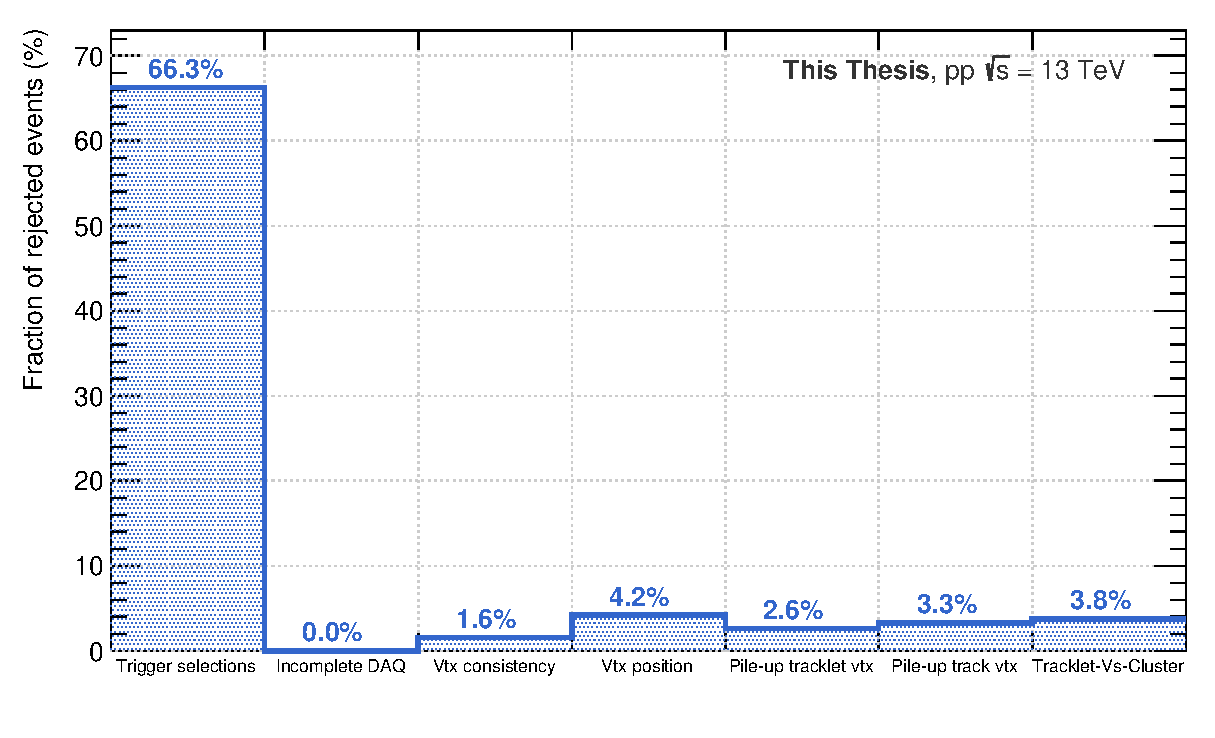
\includegraphics[width=1\textwidth]{Figs/Chapter5/EventSelection.eps}
	\caption{Fraction of rejected events in the present data sample for each event selection independently of the others: trigger selections (MB$_{\rm AND}$ and/or HM$_{\rm VZERO}$), incomplete DAQ, consistency between the global track and SPD tracklet vertices, longitudinal position of the primary vertex ($\mid \Delta z \mid < 10 $ \cm), pile-up removal for SPD tracklet and ITS-TPC track vertices, correlation between SPD tracklets and clusters.}
	\label{fig:EvtSelection}
\end{figure}


\Fig\ref{fig:EvtSelection} provides the fraction of rejected events as a function of the above selections in pp collisions at \sqrtS = 13 \tev.\\

\section{Analysis of the hyperon masses}
\label{sec:AnalysisOfHyperonMasses}

\subsection{Track selections}
\label{subsec:TrackSelections}

The identification of V0s and cascades strongly depends on the reconstruction quality of the daughter tracks, and more precisely on their momentum resolution and trajectory. For that reason, the strange particle reconstruction relies exclusively on ITS-TPC combined tracks, since they offer the best momentum resolution as discussed in \Sec\ref{subsubsec:TrackReco} and shown in \fig\ref{fig:MomResolution}. In order to ensure an excellent momentum resolution as well as a fine estimation of the particle trajectory, various selection criteria are applied on the daughter tracks.\\

The analysis concentrates exclusively on tracks comprised within the pseudo-rapidity region $\abspseudorap < 0.8$. The latter corresponds to the acceptance volume of all the central detectors, which provides a constant reconstruction efficiency. Moreover, any track containing ITS and/or TPC shared clusters is rejected, as they potentially correspond to wrongly assigned clusters that could bias the tracking quality. 

Tracks belonging to a \textit{kink} vertex are discarded from the analysis, as they most certainly do not originate from a cascade decay and thus represent an additional source of combinatorial background. A kink usually happens when a charged particle decays into a neutral and a charged particle, such as $\Kplusmin \rightarrow \rmNeutrinoMu \muPlusMinus$. The former being undetected, they are identified by forming pairs of tracks, that intersect in space with a large angle and share the same electric charge.

Each track should have passed the final refit in the TPC. This means that its parameters have been estimated successfully in the TPC during the third stage of the tracking, when the track is re-propagated inwards to their distance of closest approach to the primary vertex (\Sec\ref{subsubsec:TrackReco}). To guarantee a good momentum resolution and a stable particle identification (PID) based on the energy deposit (\dEdx) in the TPC, the tracks need to be associated to at least 70 readout pad rows in the TPC out of 159 possible in total. These selections eliminate the contribution of short tracks and, incidentally, pairs of tracks formed out of the clusters from a single actual particle.\\

The reconstruction of V0s and cascades presented in \chap\ref{chap:V0CascReconstruction} does not resort to any kind of selections on the nature of the daughter particles, apart from their electric charge. This yields \textit{de facto} to an outstanding amount of background candidates. One way of suppressing the latter with a minimal cost in terms of signal candidates consists in using the PID informations provided by the TPC. In practice, the idea is to reject every association that involves tracks inconsistent with the expected identities for either a \rmKzeroS, \rmLambdaPM, \rmXiPM or \rmOmegaPM decay.

As explained in \Sec\ref{subsubsec:TPC}, a track can be labeled as a pion, proton or kaon by making use of the PID estimator in \eq\ref{eq:PIDEstimator}, \Nsigma, which evaluates the difference between the measured \dEdx and the expected one under a given particle mass hypothesis in units of relative resolution. The separation power of such estimator evolves with the particle momentum which, in turn, influences the selection threshold and has some implications in terms of purity and efficiency: the tighter the selection on \Nsigma, the higher the purity but at the price of a smaller efficiency; conversely, a looser cut on \Nsigma deteriorates the purity in favour of a higher efficiency.

The identification strategy adopted here consists in selecting only the tracks compatible with their expected mass hypothesis within \Nsigma = $\pm 3$ at most. This selection is applied on \emph{each} decay daughters, irrespective of their momentum or the one of the mother particle. Considering the \rmXiM or \rmOmegaM case, this imposes that:
\begin{itemize}
\item[$\bullet$] the bachelor track must be consistent with the \rmPiMinus or \rmKMinus mass hypothesis, in the case of \rmXiM or \rmOmegaM respectively,
\item[$\bullet$] the positive track needs to be compatible with a proton hypothesis,
\item[$\bullet$] and the negative track has to agree with energy loss band of the pion.
\end{itemize}
In the case of \rmAxiP or \rmAomegaP, one needs to swap the electric charge of the  decay daughters, namely the positive track needs to be compatible with a pion hypothesis and the negative track, an anti-proton. For the \rmKzeroS, both positive and negative tracks should be compatible with the pion hypothesis.


\subsection{V0s and cascades selections}
\label{subsec:V0CascSelections}

\subsubsection{Topological and kinematic selections}

Once the events and tracks have been selected, the topological reconstruction of V0s and cascades comes into play, as explained in \chap\ref{chap:V0CascReconstruction}. However, not all the candidates are considered in the analysis. As suggested in \Sec\ref{subsec:HyperonAndALICE}, ALICE is well suited for studying hyperons but only at mid-rapidity. This means that the V0s and cascades are reconstructed in the rapidity window $\absrap < 0.5$.

\begin{table}[t]
    \centering
    \begin{tabular}{c|c|c}
    \noalign{\smallskip}\hline \noalign{\smallskip}
    \bf Candidate variable & Selections \rmLambdaPM & Selections \rmKzeroS \\
    \noalign{\smallskip}\hline \noalign{\smallskip}    
    V0 \pT interval (\gmom) & \multicolumn{2}{c}{1 < \pT < 5} \\
    V0 rapidity interval & \multicolumn{2}{c}{\absrap < 0.5} \\
    Competing mass rejection (\gmass) & > 0.010 & > 0.005 \\
    MC association (MC only) & \multicolumn{2}{c}{Correct identity assumption} \\ 

    \noalign{\smallskip} \hline \noalign{\smallskip}
    \bf Track variable & Selections \rmLambdaPM & Selections \rmKzeroS \\
    \noalign{\smallskip} \hline \noalign{\smallskip}
    Pseudo-rapidity interval & \multicolumn{2}{c}{\abspseudorap < 0.8} \\
    TPC refit & \multicolumn{2}{c}{\CheckGr} \\
    Nbr of crossed TPC readout rows & \multicolumn{2}{c}{ > 70} \\
    $\Nsigma^{\rm TPC}$ & \multicolumn{2}{c}{< 3} \\
    \multirow{ 2}{*}{Out-of-bunch pile-up rejection} & \multicolumn{2}{c}{at least one track with} \\
     & \multicolumn{2}{c}{ITS-TOF matching} \\
     Anterior ITS cluster rejection & \multicolumn{2}{c}{> 1 $\sigma_{\rm R}$} \\
    \noalign{\smallskip}\hline \noalign{\smallskip}
    \bf Topological variable & Selections \rmLambdaPM & Selections \rmKzeroS \\
    \noalign{\smallskip}\hline \noalign{\smallskip}
    
    V0 decay radius (\cm) & \multicolumn{2}{c}{> 0.5}\\
    V0 Lifetime (\cm) & \multicolumn{2}{c}{< 3 $\times$ \cTau}\\
    V0 cosine of pointing angle & \multicolumn{2}{c}{> 0.998}\\
    DCA proton to prim. vtx (\cm) & > 0.06 & - \\
    DCA pion to prim. vtx (\cm) & \multicolumn{2}{c}{> 0.06} \\
%    DCA V0 to prim. vtx (\cm) & < 1 & < 0.06 \\
    DCA between V0 daughters (std dev) & \multicolumn{2}{c}{< 1} \\
    
    \noalign{\smallskip}\hline \noalign{\smallskip}
    \end{tabular}
    \caption{Summary of the topological and track selections, as well as the associated cut values, used in the reconstruction of \rmLambdaPM and \rmKzeroS in pp events at \sqrtS = 13 \tev. The \textit{competing mass rejection} refers to the removal of the background contamination from other mass hypotheses (\Sec\ref{subsubsec:InvariantMassSelection}). In the \rmLambdaPM case, this consists in comparing the invariant mass under the assumption of a \rmPiPlus\rmPiMinus and PDG mass of \rmKzeroS, that is the quantity $\mid\mInv[\rm hyp.\ \rmKzeroS] - \mPDG[\rmKzeroS]|$. When reconstructing \rmKzeroS candidates, the selection variable becomes $\mid\mInv[\rm hyp.\ \rmLambda] - \mPDG[\rmLambda]|$.}\label{tab:V0Selections}
\end{table}

The above selections on the track quality in TPC exclude the possibility of studying the particles of interest at low momentum ($\pT \leq 0.6$ \gmom). At such values, the V0s and cascades decay into very low momentum tracks, that can only be reconstructed via the ITS standalone tracking. Even when these tracks reach the TPC, they form short tracks and are thus rejected (\Sec\ref{subsec:TrackSelections}). As a matter of fact, in order to secure a reasonably good momentum resolution on the decay daughters, this analysis only considers candidates from 1 to 5 \gmom. On the one hand, \eq\ref{eq:Gluckstern} indicates that the momentum resolution deteriorates at low momentum ($\pT \leq 1$ \gmom) due to their relatively \say{short} track length, \say{small} number of clusters and the dominant contribution of multiple scattering. On the other hand, at high \pT ($\pT \geq 5$ \gmom), the resolution also decreases as a consequence of less pronounced track curvature.\\

\begin{table}[p]
    \centering
    \begin{tabular}{c|c|c}
    \noalign{\smallskip}\hline \noalign{\smallskip}
    \bf Candidate variable & Selections \rmXiPM & Selections \rmOmegaPM \\
    \noalign{\smallskip}\hline \noalign{\smallskip}    
    Cascade \pT interval (\gmom) & \multicolumn{2}{c}{1 < \pT < 5} \\
    Cascade rapidity interval & \multicolumn{2}{c}{\absrap < 0.5} \\
    Competing mass rejection (\gmass) & - & > 0.008 \\
    MC association (MC only) & \multicolumn{2}{c}{Correct identity assumption} \\ 

    \noalign{\smallskip}\hline \noalign{\smallskip}
    \bf Track variable & Selections \rmXiPM & Selections \rmOmegaPM \\
    \noalign{\smallskip}\hline \noalign{\smallskip}
    Pseudo-rapidity interval & \multicolumn{2}{c}{\abspseudorap < 0.8} \\
    TPC refit & \multicolumn{2}{c}{\CheckGr} \\
    Nbr of crossed TPC readout rows & \multicolumn{2}{c}{ > 70} \\
    $\Nsigma^{\rm TPC}$ & \multicolumn{2}{c}{< 3} \\
    \multirow{ 2}{*}{Out-of-bunch pile-up rejection} & \multicolumn{2}{c}{at least one track with} \\
     & \multicolumn{2}{c}{ITS-TOF matching} \\
    Anterior ITS cluster rejection & \multicolumn{2}{c}{> 1 $\sigma_{\rm R}$} \\
    \noalign{\smallskip}\hline \noalign{\smallskip}
    \bf Topological variable & Selections \rmXiPM & Selections \rmOmegaPM \\
    \noalign{\smallskip}\hline \noalign{\smallskip}
    
    \multicolumn{3}{l}{\textbf{V0}} \\
    V0 decay radius (\cm) & > 1.2 & > 1.1\\
    V0 cosine of pointing angle & \multicolumn{2}{c}{> 0.97}\\
    |$m$(V0) - \mPDG[\rmLambda]| (\gmass) & \multicolumn{2}{c}{< 0.008} \\
    DCA proton to prim. vtx (\cm) & \multicolumn{2}{c}{> 0.03} \\
    DCA pion to prim. vtx (\cm) & \multicolumn{2}{c}{> 0.04} \\
    DCA V0 to prim. vtx (\cm) & \multicolumn{2}{c}{> 0.06} \\
    DCA between V0 daughters (std dev) & \multicolumn{2}{c}{< 1.5} \\
    \noalign{\smallskip}\hline \noalign{\smallskip}
    
    \multicolumn{3}{l}{\textbf{Cascade}} \\
    Cascade decay radius (\cm) & > 0.6 & > 0.5 \\
    Cascade Lifetime (\cm) & \multicolumn{2}{c}{< 3 $\times$ \cTau}\\
    DCA bachelor to prim. vtx (\cm) & \multicolumn{2}{c}{> 0.04} \\
    DCA between cascade daughters (std dev) & \multicolumn{2}{c}{< 1.3} \\
    Cascade cosine of pointing angle & \multicolumn{2}{c}{> 0.998} \\
    Bachelor-proton pointing angle (rad) & \multicolumn{2}{c}{> 0.04} \\
    
    \noalign{\smallskip}\hline \noalign{\smallskip}
    \end{tabular}
    \caption{Summary of the topological and track selections, as well as the associated cut values, used in the reconstruction of \rmXiPM and \rmOmegaPM in pp events at \sqrtS = 13 \tev. The \textit{competing mass rejection} refers to the removal of the background contamination from other cascade hypothesis (\Sec\ref{subsubsec:InvariantMassSelection})}\label{tab:CascadeSelections}
\end{table}


To further remove the contribution from out-of-bunch pile-up events, it is required that at least one of the daughter tracks to either have a cluster in the innermost ITS layers\footnote{Technically, it is requested to have passed the final refit in the ITS and to have a hit in one of the two SPD layers.} or match with a hit in the TOF. The former uses the fast readout time of the SPD to limit the pile-up to tracks produced in collisions within~$\pm$~300~\nsec, that is $\pm$ 12 bunch crossings\footnote{Keep in mind that, in ALICE during the LHC Run-2, the average number of collisions per bunch crossing is not about 30-50 as for ATLAS and CMS, or 1-2 for LHCb; it is smaller than 1-5\%, \ie a low trend in terms of pile-up.}; the latter exploits the highly precise timing information of the TOF to identify the bunch crossing from which the particle originates, with an efficiency of approximately 70 to 80\% for intermediate or high \pT particles and drops rapidly for lower momentum due to mismatches \cite{alicecollaborationALICEDPGPileup2021}. This selection has been thoroughly studied in the context of a strange particle production analysis \cite{alicecollaborationMultiplicityDependenceMulti2020}; it was shown that applying this ITS-TOF matching condition on at least one of the decay daughters is sufficient to eliminate most of the remaining pile-up contamination.\\

Moreover, the reconstruction procedure presented in the \chap\ref{chap:V0CascReconstruction} corresponds to a so-called \emph{offline} reconstruction: V0s and cascades are formed by combining tracks, that have already been reconstructed during the event reconstruction (\Sec\ref{subsec:EventReco}). However, during the tracking stage, there is no way to know \textit{a priori} that they actually originate from a hyperon; they are thus reconstructed as any other track in the event. As a consequence, there is no causality check\footnote{There is, however, a causality check performed in the cascade reconstruction in order to ensure that the V0 decay point does not sit downstream from the cascade decay position.} against assigned ITS clusters anterior to the V0 and/or cascade decays. Due to the possible bias that might be introduced in the invariant mass of the mother particle, all the daughter tracks updated with an ITS cluster \emph{below} the associated decay point by more than~1~$\sigma_{\rm R}$\footnote{$\sigma_{\rm R}$ refers to the resolution on the radial decay position of the V0 or cascade.} are discarded. This requirement applies for both V0 and cascade candidates.

In summary, \tabs\ref{tab:V0Selections} and \ref{tab:CascadeSelections} provide a list of the track and topological selections employed in the reconstruction of V0s and cascades respectively, as well as the numerical cut values. Note the tight cut on the cosine of pointing angle of the cascade candidate; this is discussed later in \Sec\ref{subsec:MassExtraction}.

\subsubsection{Structure in the invariant mass spectrum of cascades}
\label{subsubsec:InvMassStructure}

Among the topological selections listed in \tab\ref{tab:CascadeSelections}, one of them has not been introduced and discussed in \chap\ref{chap:V0CascReconstruction}, namely the cut on the pointing angle formed by the bachelor and the positive particles. Contrarily to the other selections, this one is not standard in ALICE; it has been introduced in 2020 by \cite{silvadealbuquerqueMultistrangeHadronsPb2019}. At that time, a structure in the invariant mass distribution of \rmXi and \rmOmega, similar to the one in \figs\ref{fig:WrongPA}, was observed in Pb-Pb collisions. It turned out that the bump background, between 1.28 and 1.31 \gmass on \figs\ref{fig:XiMinusWrongPA} and \ref{fig:XiPlusWrongPA}, originates from an erroneous track association in the cascade reconstruction. 

A V0 decays into a baryon \proton/\pbar and a \rmPiMinus/\rmPiPlus, depending on whether this is a \rmLambda or \rmAlambda. In the situation where another negative/positive track in the event passes close by the proton/anti-proton, the reconstruction algorithm may interpret that as a V0~decay; this track plays the role of the negative/positive daughter particle of a \rmLambdaPM, and the proton/anti-proton corresponds to its positive/negative daughter particle. On the other hand, the remaining \rmPiMinus/\rmPiPlus daughter of the actual \rmLambdaPM is combined to other particles, and most likely to the previously ill-formed V0. In such case, it acts like the bachelor particle of a cascade decay. In other words, while the actual topology is depicted in \fig\ref{fig:WrongV0}, it is reconstructed as a cascade, as illustrated in \fig\ref{fig:TrueV0}.

The analysis in \cite{silvadealbuquerqueMultistrangeHadronsPb2019} investigated different strategies in order to remove this background contamination. In the end, the best option consists in rejecting candidates with a \emph{small} pointing angle for the dummy V0, \ie the pointing angle formed by the V0 made of the bachelor and the proton, as shown in \fig\ref{fig:WrongPACut}.


\begin{figure}[t]
\hspace*{-1.5cm}
\subfigure[]
{
	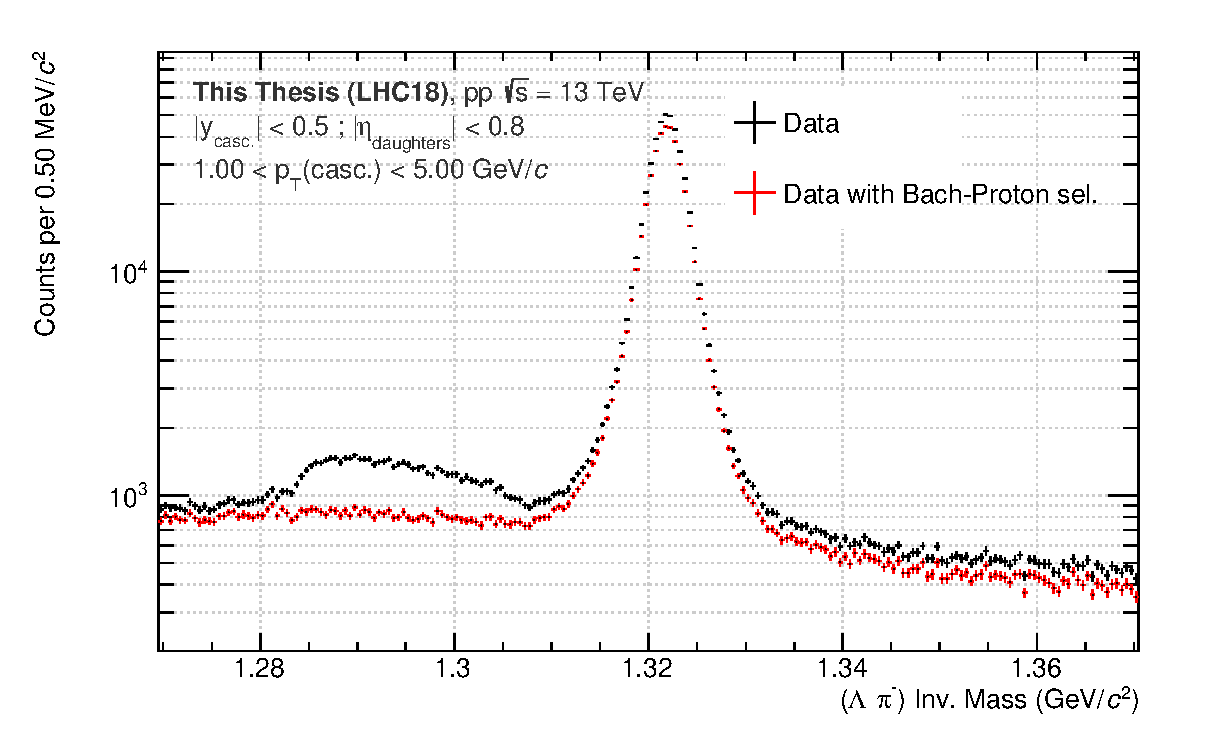
\includegraphics[width=0.6\textwidth]{Figs/Chapter5/InvMassXiMinus_WrongPA.eps}
	\label{fig:XiMinusWrongPA}
}
\subfigure[]
{
	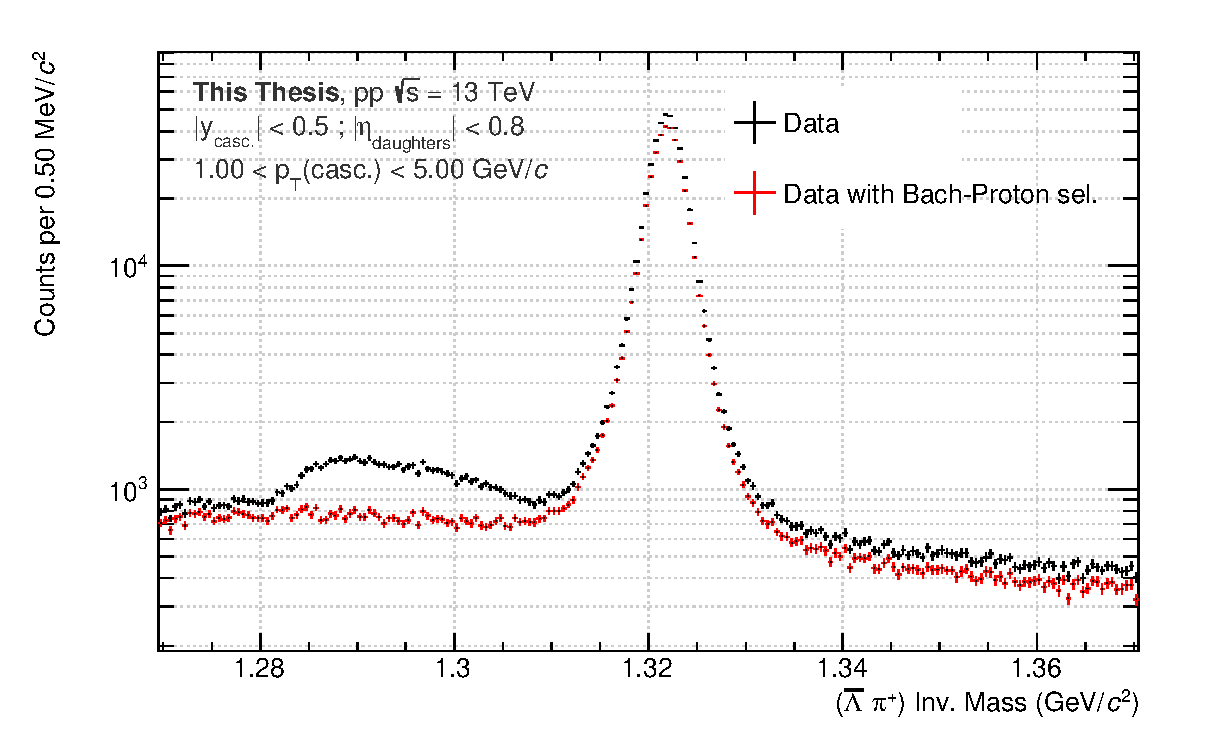
\includegraphics[width=0.6\textwidth]{Figs/Chapter5/InvMassXiPlus_WrongPA.eps}
	\label{fig:XiPlusWrongPA}
}
\hspace*{-1.5cm}	
\subfigure[]
{
	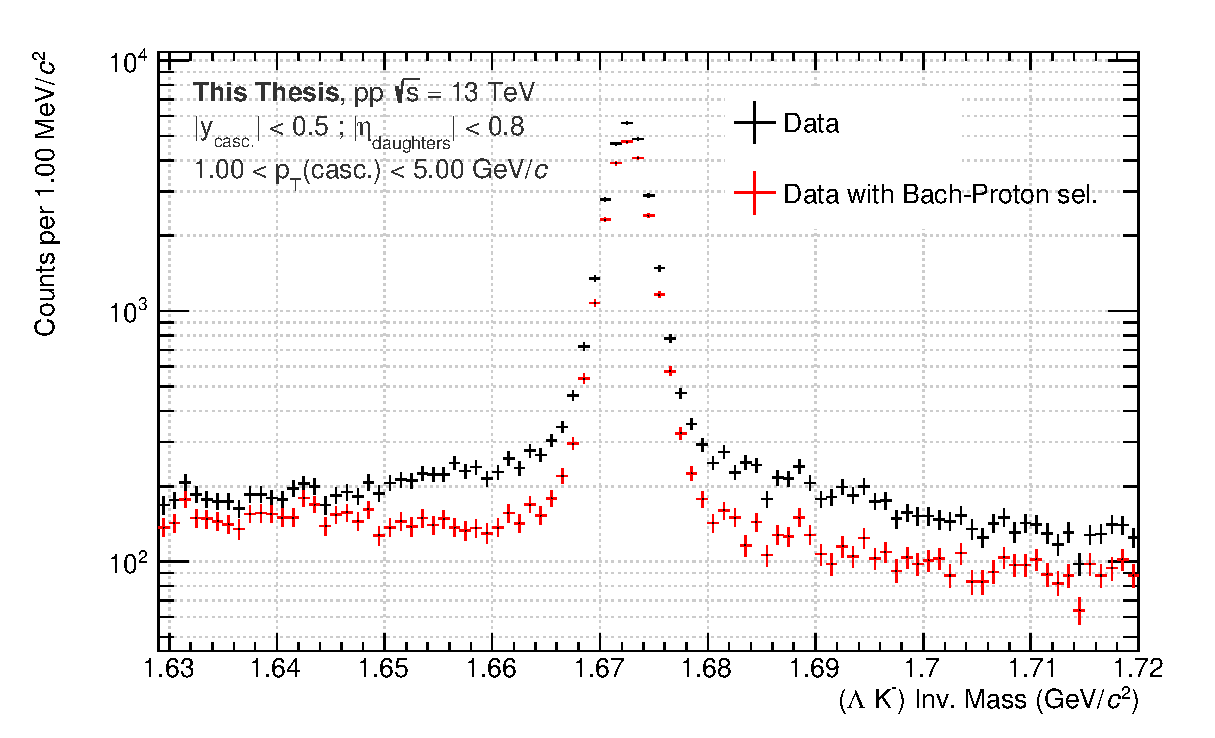
\includegraphics[width=0.6\textwidth]{Figs/Chapter5/InvMassOmegaMinus_WrongPA.eps}
	\label{fig:OmegaMinusWrongPA}
}
\subfigure[]
{
	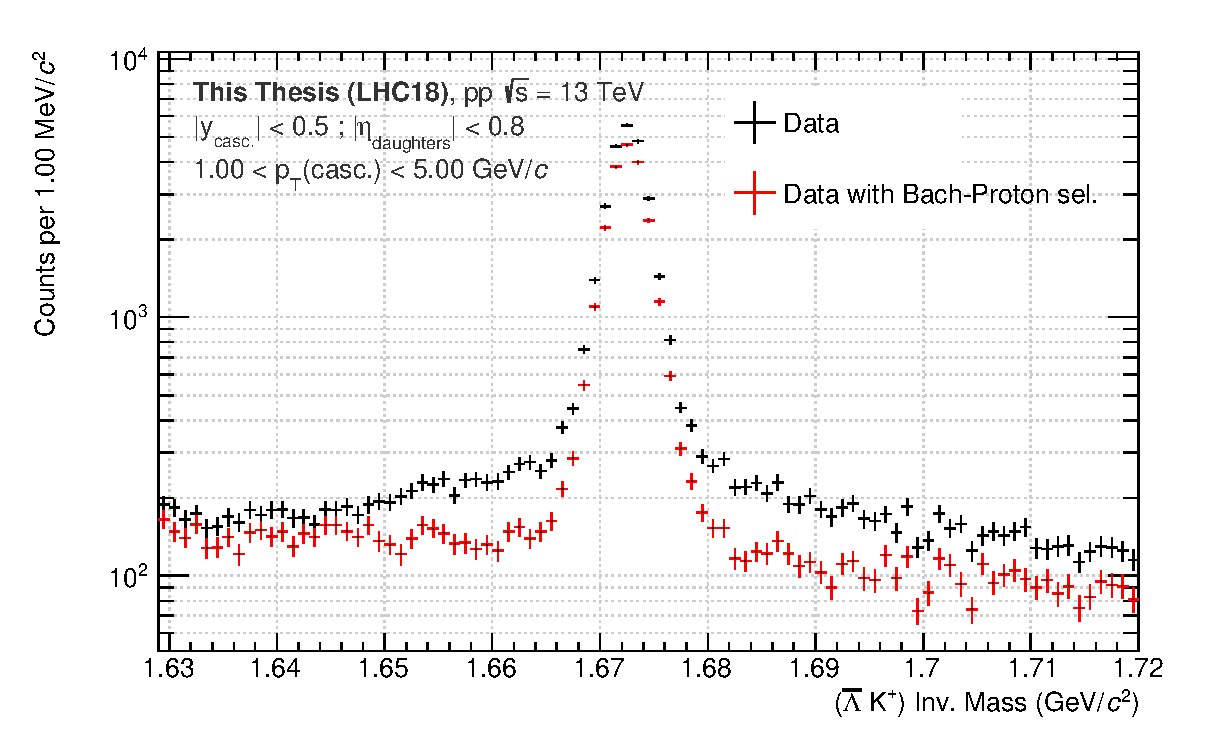
\includegraphics[width=0.6\textwidth]{Figs/Chapter5/InvMassOmegaPlus_WrongPA.eps}
	\label{fig:OmegaPlusWrongPA}
}	
	\caption{Invariant mass distribution of \rmXiM (a), \rmAxiP (b), \rmOmegaM (c) and \rmAomegaP (d) in pp at \sqrtS = 13 \tev. These have been obtained using the cuts in \tab\ref{tab:CascadeSelections} (red markers), and also without the bachelor-proton pointing angle selection (black markers). This comparison shows the latter selection removes a structure in the invariant mass distribution while preserving the population under the peak. Notice the log-scale on the y-axis, that puts into perspective the signal and background levels.}
	\label{fig:WrongPA}
\end{figure}

%\begin{figure}[t]
%    \begin{minipage}[t]{.3\textwidth}
%%        \centering
%\hspace*{-2.cm}
%        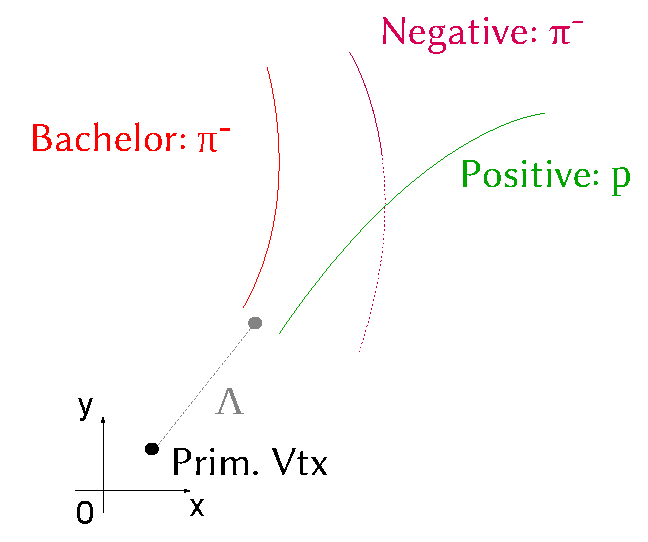
\includegraphics[width=1.25\textwidth]{Figs/Chapter5/WrongV0.eps}
%        \subcaption{Image 1.}
%	\label{fig:WrongV0}
%    \end{minipage}
%%    \hfill
%    \begin{minipage}[t]{.3\textwidth}
%%        \centering
%	\hspace*{-0.5cm}
%        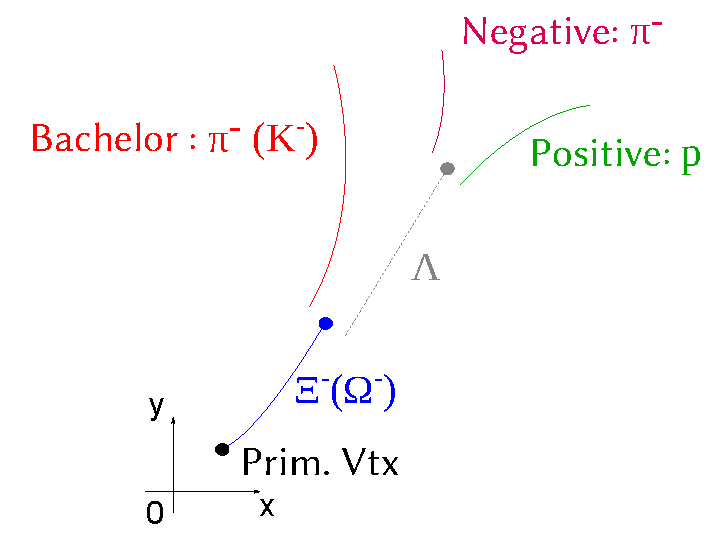
\includegraphics[width=1.35\textwidth]{Figs/Chapter5/TrueV0.eps}
%%        \subcaption{Image 1.}
%	\label{fig:TrueV0}
%    \end{minipage}  
%    \begin{minipage}[t]{.3\textwidth}
%%        \centering
%	\hspace*{1.5cm}
%        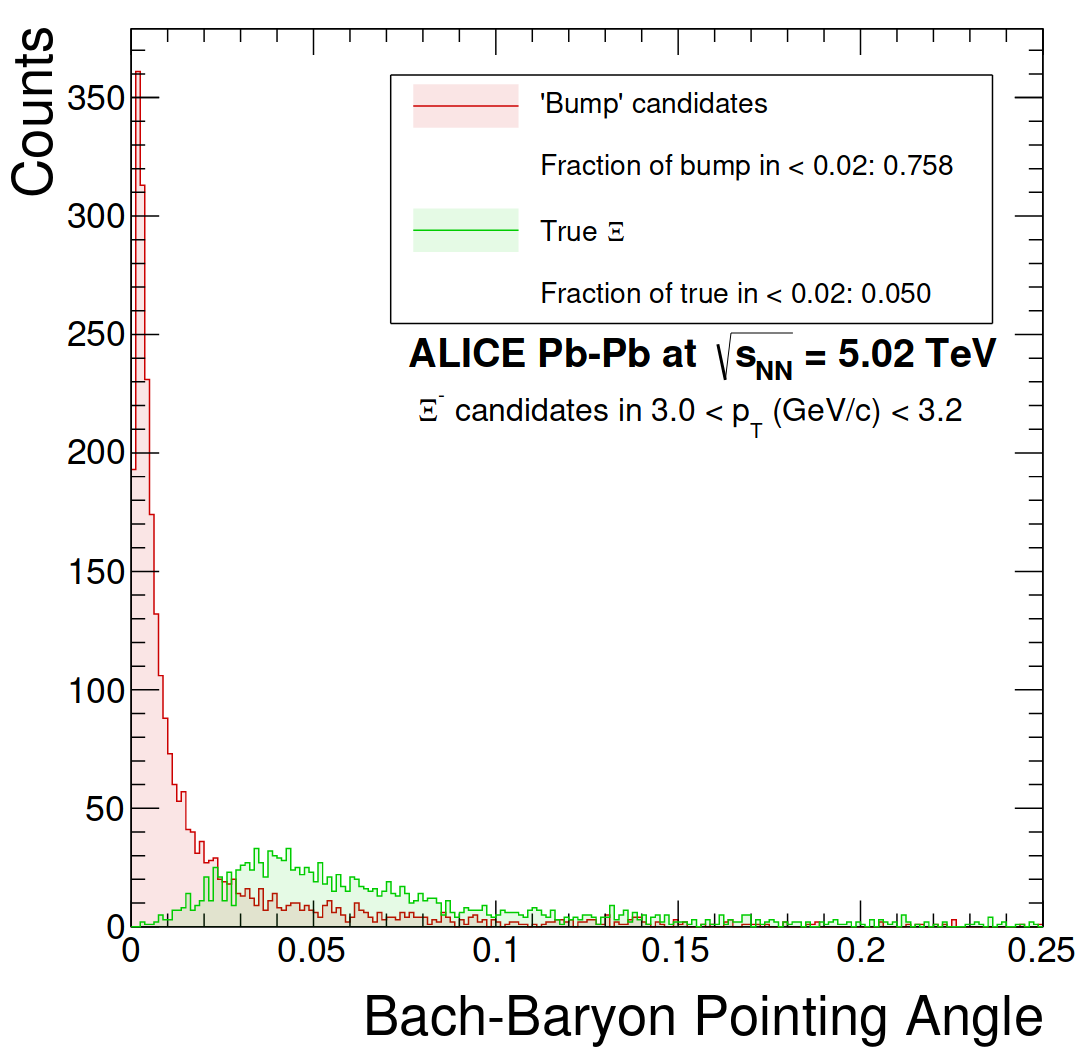
\includegraphics[width=1.45\textwidth]{Figs/Chapter5/WrongPACut.png}
%%        \subcaption{Image 1.}
%	\label{fig:WrongPACut}
%    \end{minipage}  
%    \caption{Illustrations of a \rmLambda decaying into a proton and a pion, with another pion passing close to the proton (a), identified as a cascade decay topology and reconstruted as such (b). (c) Distribution of the pointing angle formed by the bachelor and proton tracks for true associated \rmXi and for candidates in the background structure in the invariant mass distributions ("bump").}
%\end{figure}

\begin{figure}[t]
\centering
%\hspace*{-2.0cm}
\subfigure[]
{
	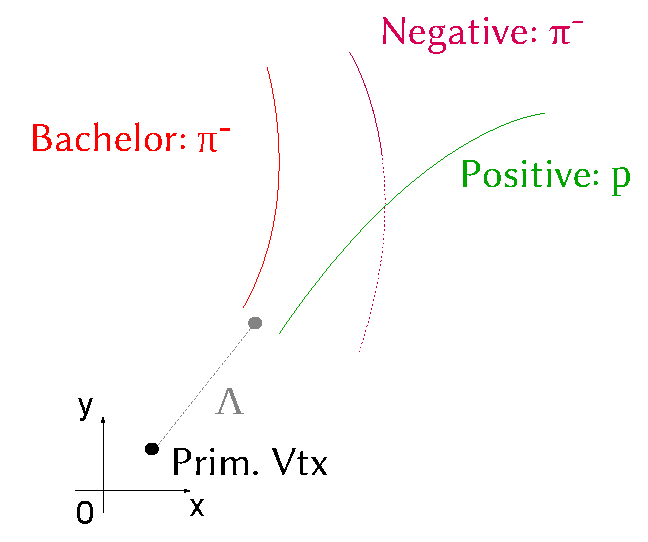
\includegraphics[width=0.4\textwidth]{Figs/Chapter5/WrongV0.eps}
	\label{fig:WrongV0}
}
\subfigure[]
{
	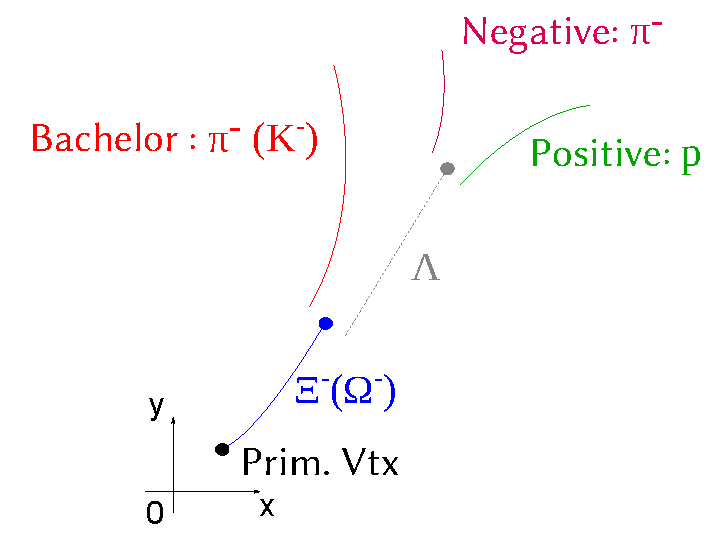
\includegraphics[width=0.45\textwidth]{Figs/Chapter5/TrueV0.eps}
	\label{fig:TrueV0}
}\\
\subfigure[]
{
	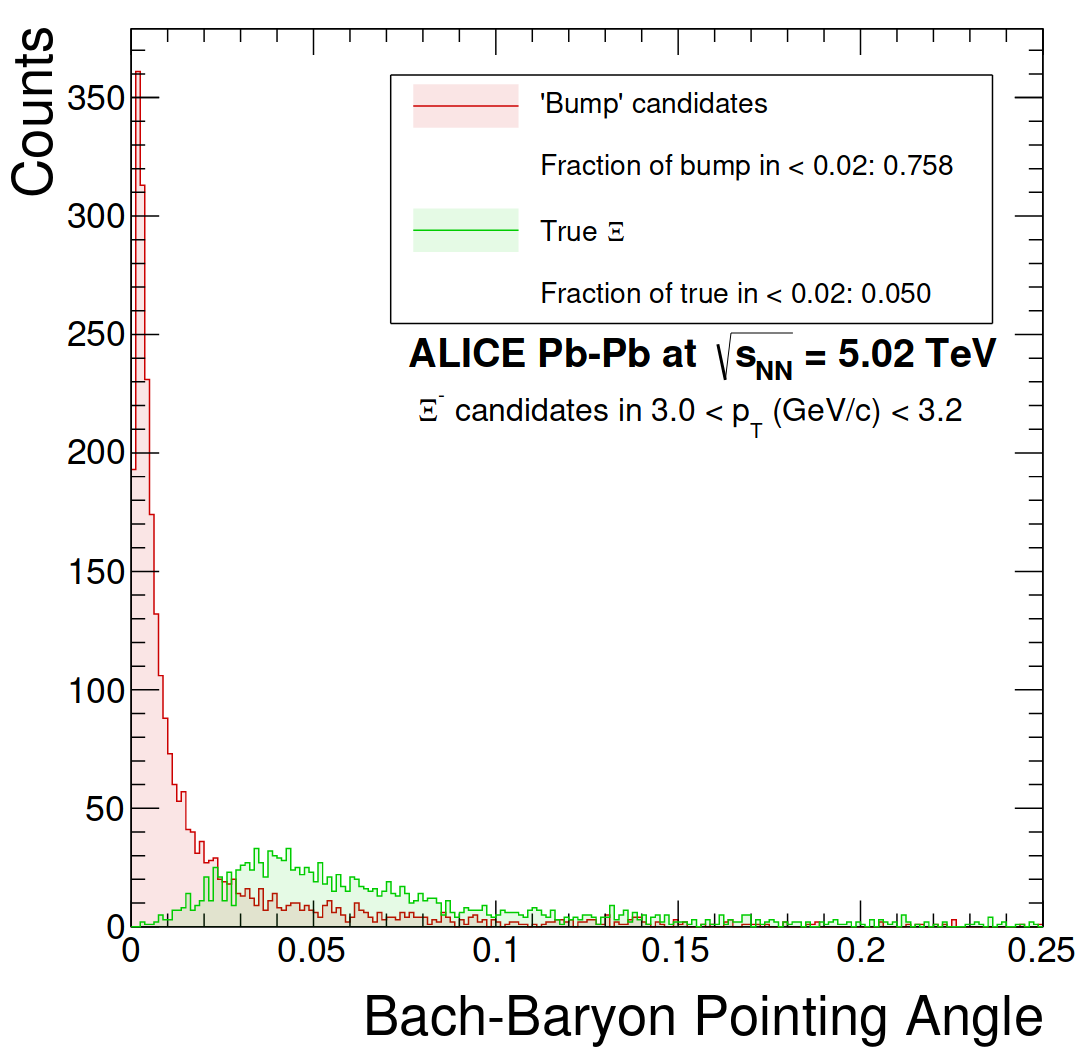
\includegraphics[width=0.5\textwidth]{Figs/Chapter5/WrongPACut.png}
	\label{fig:WrongPACut}
}
	\caption{Illustrations of a \rmLambda decaying into a proton and a pion, with another pion passing close to the proton (a), identified as a cascade decay topology and reconstruted as such (b). (c) Distribution of the pointing angle formed by the bachelor and proton tracks for true associated \rmXi and for candidates in the background structure in the invariant mass distributions ("bump").}
	\label{fig:WrongTopology}
\end{figure}

\subsection{Mass measurement}
\label{subsec:MassExtraction}

\subsubsection{Principles of the mass extraction}
\label{subsubsec:PrinciplesOfMassExtraction}

Out of all the candidates passing the above selection criteria, there contain true V0s/cascades -- depending on the particle of interest -- and background candidates. Taken individually, they are undistinguishable. The separation of these two can only be achieved statistically, based on the analysis of the invariant mass spectrum.

The invariant mass of each candidate is calculated, as explained in \Sec\ref{subsubsec:CascadeFormation} and \Sec\ref{subsubsec:InvariantMassSelection}, and sorted according to their electric charge in order to separate the particles from the anti-particles. The V0s being electrically neutral, they follow a different approach: since the \rmKzeroS decays into two particles of the same nature --- a \rmPiPlus and a \rmPiMinus ---, it is hopeless to try separating particles and anti-particles. This is not the case of \rmLambda and \rmAlambda, though. However, it may happen that the same V0 candidate passes the particle and anti-particle selections in \tab\ref{tab:V0Selections}. To avoid such double-counting, each candidate needs to go through the \rmLambda selections first. If it satisfies all conditions, it is labeled as \rmLambda and we move to the next candidate. Otherwise, it is checked against the requirements for a \rmAlambda baryon.

On one hand, most of the background candidates originate from a random association of two or three tracks. Those tracks being uncorrelated, the corresponding invariant mass spectrum should be flat or decreasing with the invariant mass value. On the other hand, the invariant mass of true V0s/cascades should be close to the tabulated mass \mPDG, such that there emerges an overpopulated region taking the shape of a peak. \Figs\ref{fig:InvMassCascades} show the invariant mass spectra of \rmXi and \rmOmega.  One can see that the signal for each species sits on top of a small background.\\

To isolate the signal from the background, a fit of the invariant mass spectra is performed using a sum of two functions: one for modeling the signal peak, the other for describing the background. Several functions can be considered, as discussed in \Sec\ref{subsubsec:SignalShape}. In \figs\ref{fig:InvMassCascades}, the peak is represented by a triple Gaussian \cite{atlascollaborationKs02012} and the background by an exponential function. Whatever the choosen functions are, the fitting procedure is performed with the maximum (log-)likelyhood method.

If the procedure manages to converge, this fit allows to measure the mass of the considered particle: it corresponds to the centre of the invariant mass peak, given by the position of the maximum of the signal function denoted as $\mu$. The width of the peak -- the parameter $\sigma$ -- provides an estimation of the experimental resolution on the mass. The uncertainties on both quantities come from the errors returned by the fitting procedure.

From these parameters, two regions of interest can be delimited:
\begin{itemize}
\item[$\bullet$] the peak region, containing all the signal\footnote{More precisely, considering the definition of the peak region in this analysis, it should contain approximately 99.99995\% (\ie a $5 \sigma$ significance level) of the true V0s/cascades measured.} and some background, is defined within $\left[ \mu - 5 \sigma ; \mu + 5 \sigma \right]$;
\item[$\bullet$] the side-bands region, solely constituted of background, consists in two bands of the same width\footnote{As a side note: the two side-bands do not need to be of the same size, but it avoids dealing with a scaling factor when comparing their total area to the one in the peak region. Most often, they have different widths because of an asymmetry in the invariant mass distribution, such as the structure reported in \Sec\ref{subsubsec:InvMassStructure} \cite{alicecollaborationProductionLightflavorHadrons2021}.}, surrounding the peak region and covering the range $\left[ \mu - 12 \sigma ; \mu - 7 \sigma \right] \bigcup \left[ \mu + 7 \sigma ; \mu + 12 \sigma \right]$.
\end{itemize}
Hence, the amount of raw signal and background can be evaluated. The peak ($S+B$) and background ($B$) populations are estimated by counting the
number of candidates in their respective regions. The raw signal ($S$) in the peak region is obtained by subtracting the background from the peak population, that is\break $S=(S+B)-B$.

\begin{figure}[p]
%\centering
\hspace*{-1.5cm}
\subfigure[]{
	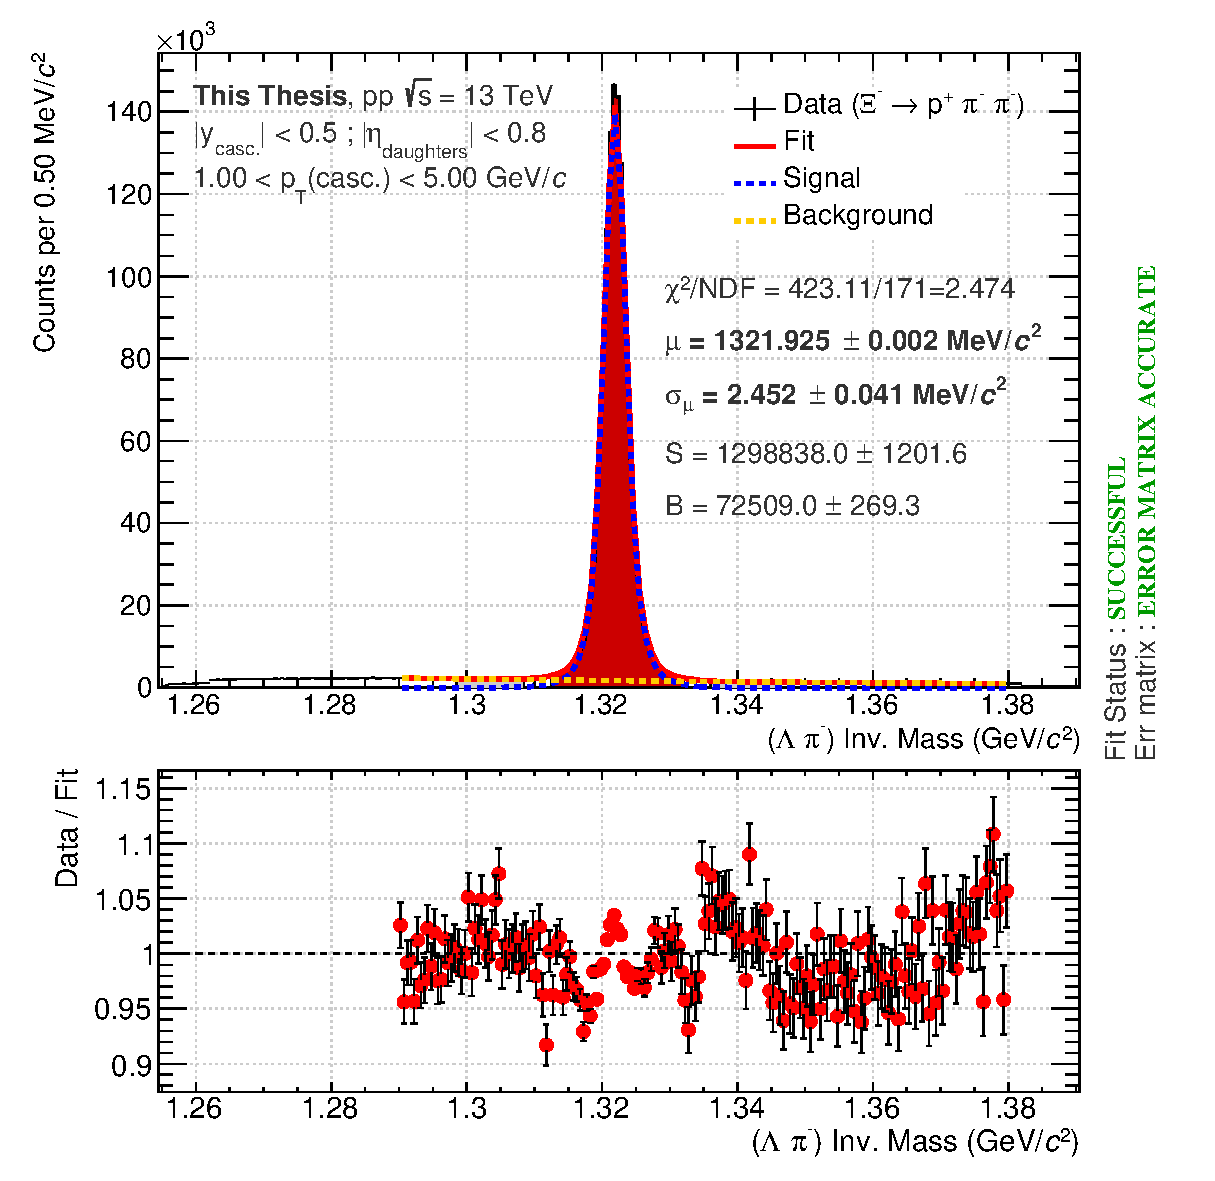
\includegraphics[width=0.6\textwidth]{Figs/Chapter5/InvMassXiMinus.eps}
	\label{fig:XiMinus_TripleGaussian}
} 
\subfigure[]{
	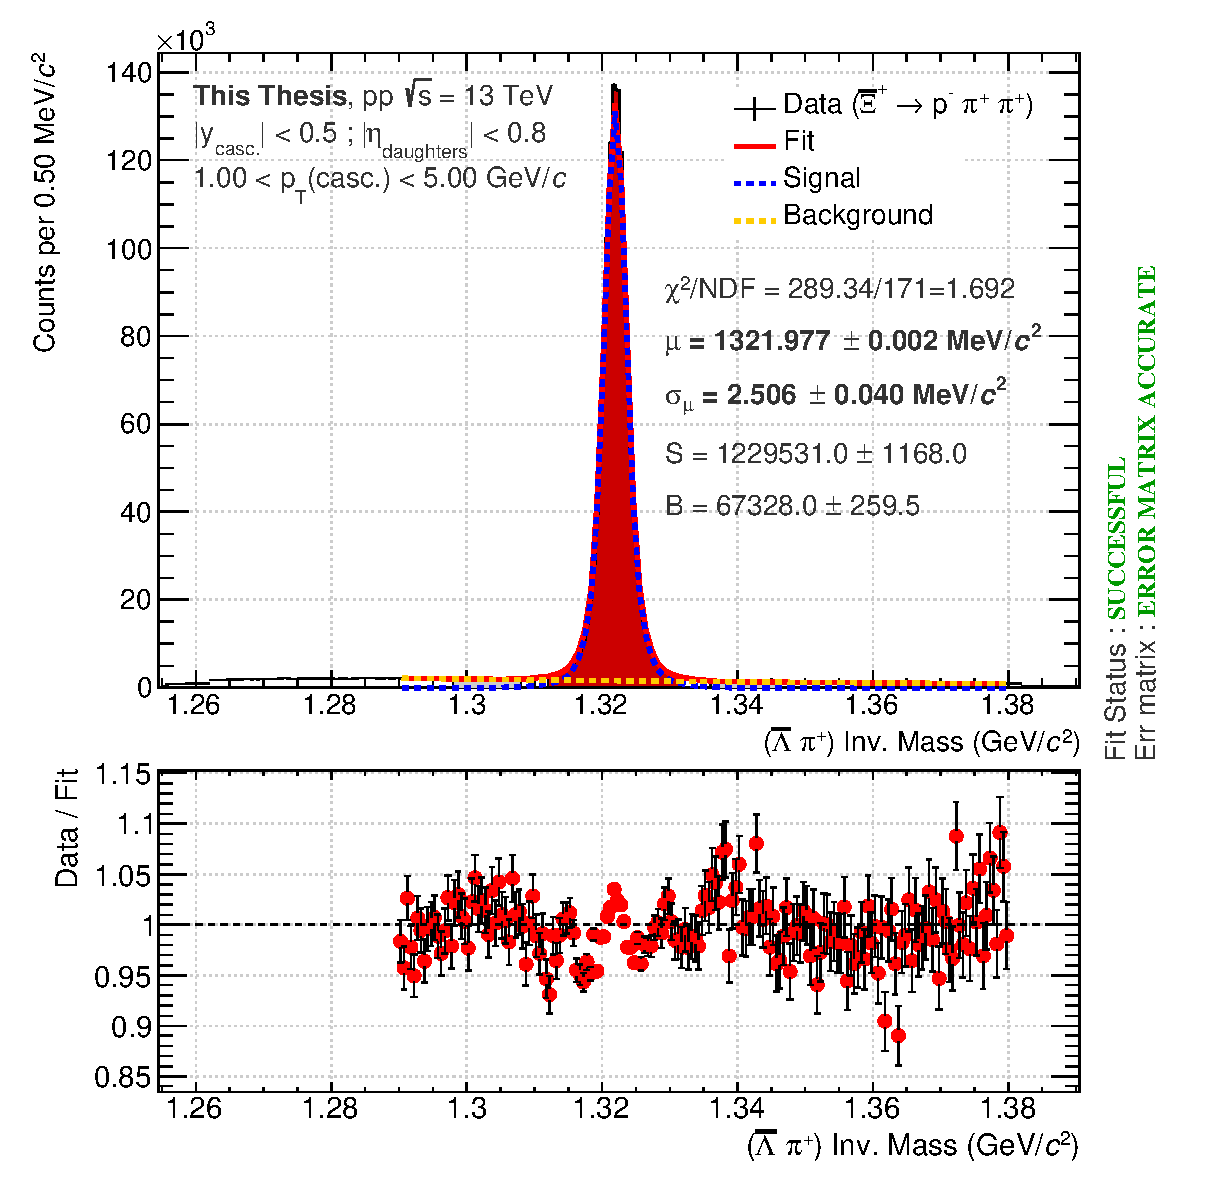
\includegraphics[width=0.6\textwidth]{Figs/Chapter5/InvMassXiPlus.eps}
	\label{fig:XiPlus_TripleGaussian}
} 
\hspace*{-1.5cm}
\subfigure[]{
	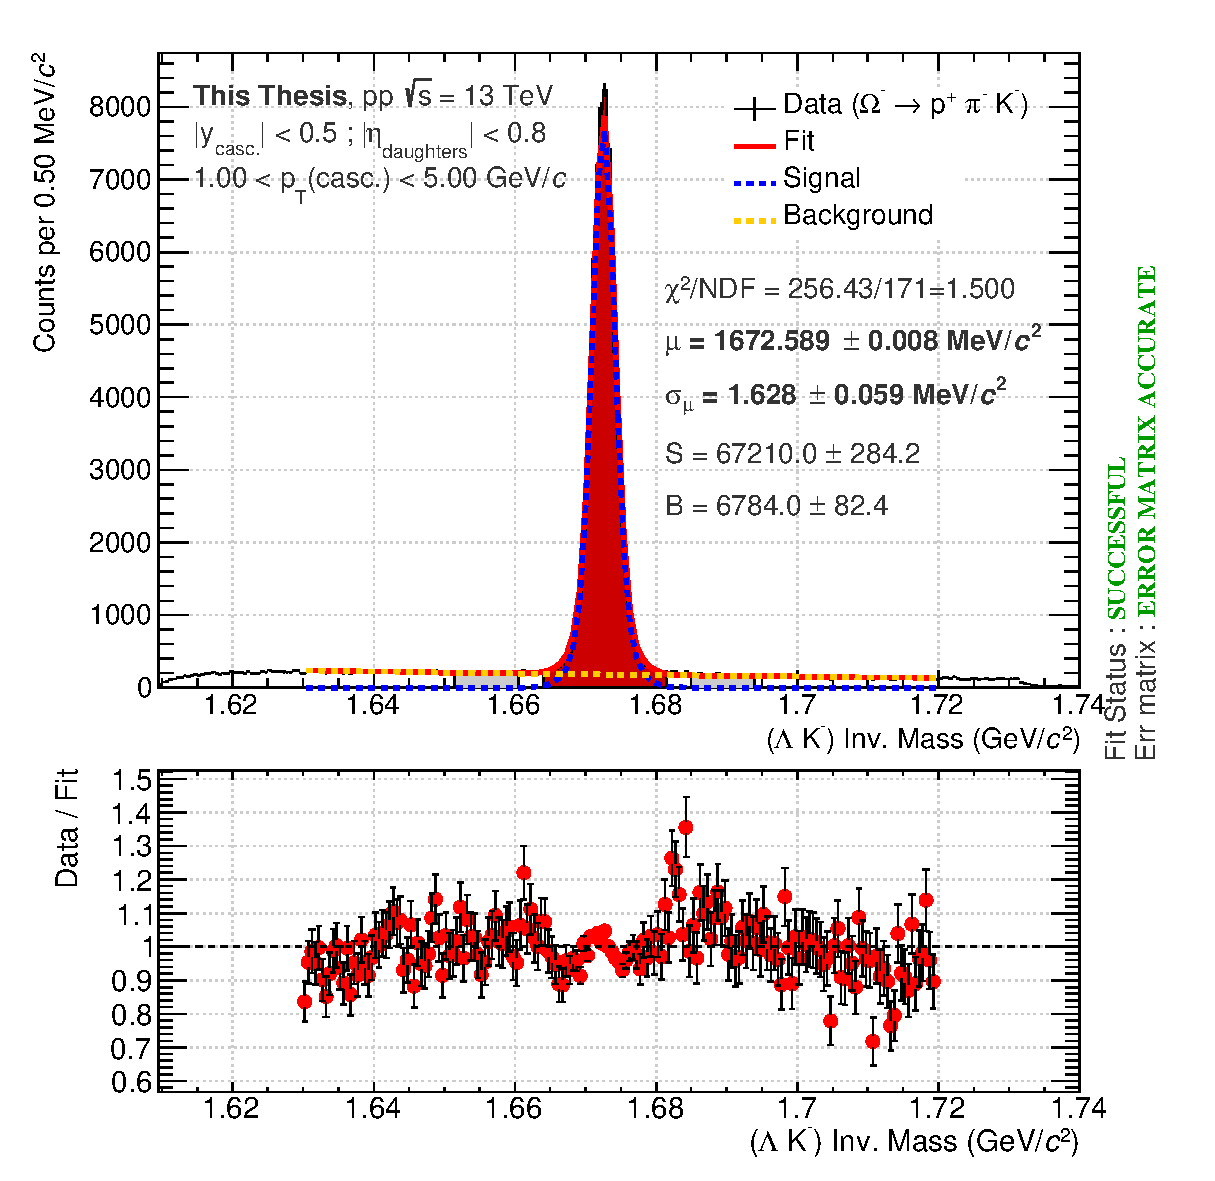
\includegraphics[width=0.6\textwidth]{Figs/Chapter5/InvMassOmegaMinus.eps}
	\label{fig:OmegaMinus_TripleGaussian}
} 
\subfigure[]{
	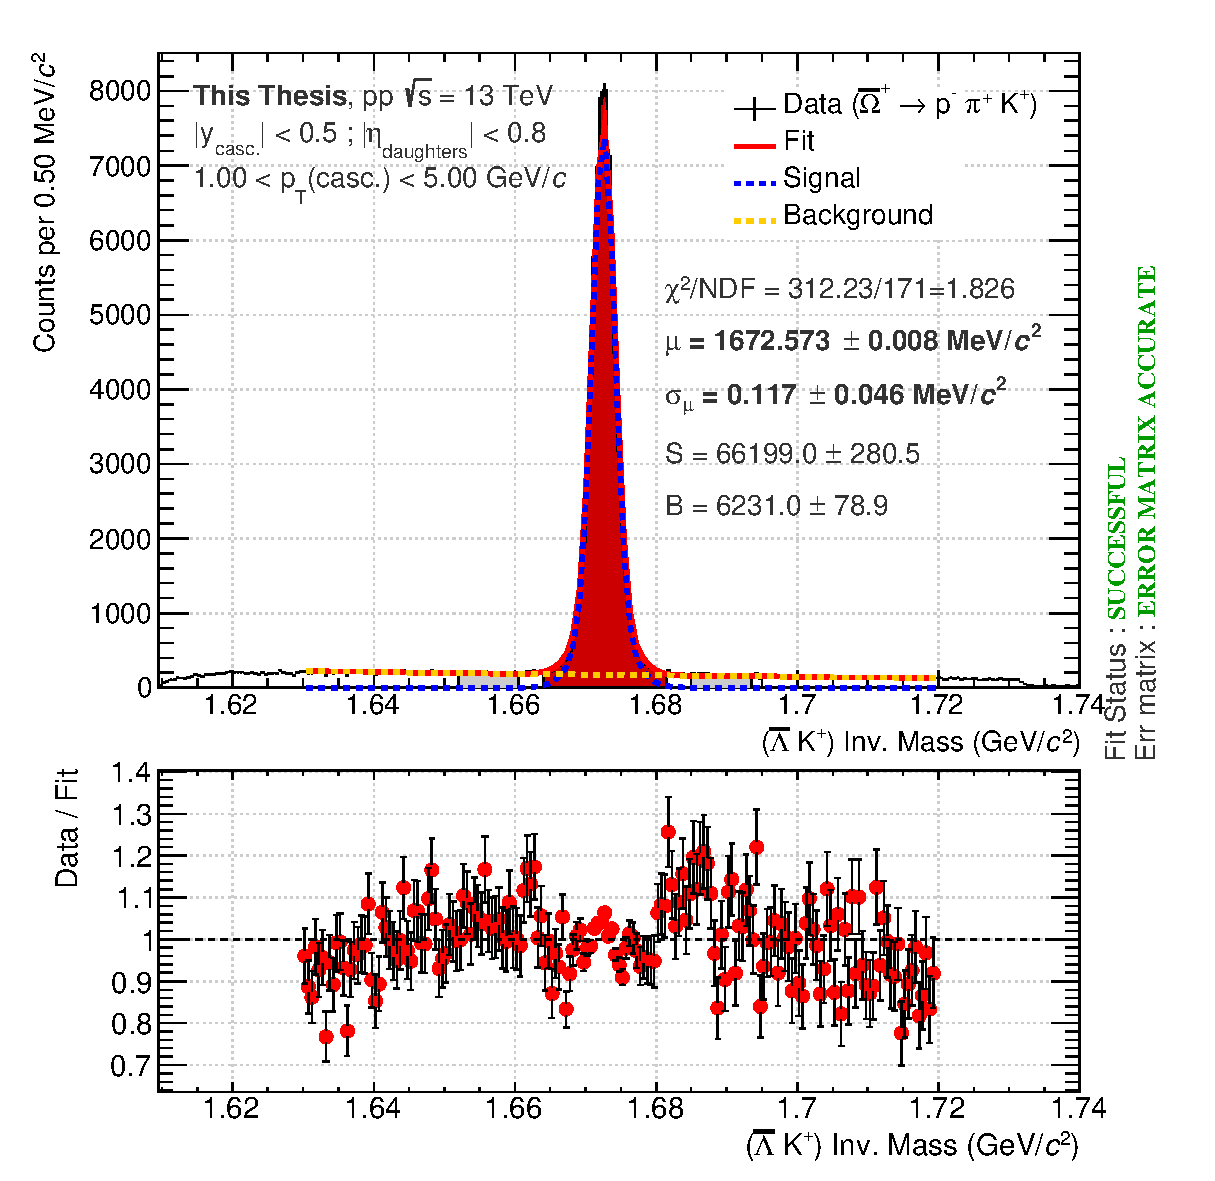
\includegraphics[width=0.6\textwidth]{Figs/Chapter5/InvMassOmegaPlus.eps}
	\label{fig:OmegaPlus_TripleGaussian}
}  
\caption{Invariant mass distributions of \rmXiM (a), \rmAxiP (b), \rmOmegaM (c) and \rmAomegaP (d) hyperons in pp collisions at \sqrtS = 13 \tev. Here, the peak is modeled by a triple Gaussian, and the background by an exponential function. Each distribution comes with an additional panel representing the consistency between the data and the fit model, in the form of a ratio per invariant mass bin. The error bars encompasses the uncertainties on both quantities.}
	\label{fig:InvMassCascades}
\end{figure}

In \figs\ref{fig:InvMassCascades}, all the fits are of reasonably good quality\footnote{One may argue that, in the case of the \rmXiM, the reduced $\chi^{2}$  is relatively high. However, the comparison of the bottom panels of the \rmXiM and \rmAxiP allows to conclude that it certainly comes from a slightly worst description of the background.}. The bottom panels show that the data-model discrepancy does not exceed 5\% for the most precise points, \ie those in the peak region. The mass peak sits on a small background: 1~298~838~$\pm$~1202~\rmXiM (1~229~531~$\pm$~1168~\rmAxiP) and 67~210~$\pm$~285~\rmOmegaM (66~199~$\pm$~281~\rmAomegaP) were reconstructed with purities above 90\%, as shown in \tab\ref{tab:FitQuantities}.

\begin{table}[h]
    \centering
    \begin{tabular}{b{5.35cm}@{\hspace{1cm}} b{2cm}@{\hspace{0.5cm}} b{2cm}@{\hspace{0.5cm}} b{1.5cm}@{\hspace{0.5cm}} b{1.5cm}@{\hspace{0.1cm}}}
    \noalign{\smallskip}\hline\noalign{\smallskip}
	\bf Particle & \rmXiM & \rmAxiP & \rmOmegaM & \rmAomegaP \\	
    \noalign{\smallskip}\hline \noalign{\smallskip}
    Reduced $\chi^2$ & 2.474 & 1.692 & 1.500 & 1.826\\
    	Raw signal, $S$ &  1 298 838 & 1 229 531 & 67 210 & 66 199\\
    	Background, $B$ & 75209 & 67 328 & 6784 & 6231 \\
    	$S/B$ & 17.3 & 16.4 & 9.91 & 10.63 \\
    	Purity, $S/(S+B)$ & 94.5\% & 94.2\% & 90.8\% & 91.4\% \\
    Signal significance, $S/\sqrt{S+B}$ & 1108 & 1076 & 247 & 246 \\
    \noalign{\smallskip}\hline\noalign{\smallskip}
    \end{tabular}
    \caption{Results from the fit of the invariant mass distributions in \fig\ref{fig:InvMassCascades} concerning the overall samples of \rmXiM, \rmAxiP, \rmOmegaM and \rmAomegaP. Therefore, this table reports the reduced $\chi^{2}$, raw signal, background, ratio $S/B$, purity and signal significance.}\label{tab:FitQuantities}
\end{table}

\subsubsection{Shape of the peak functions}
\label{subsubsec:SignalShape}

Since the mass extraction depends on the peak description, it is crucial to identify functional forms that reproduce accurately its shape. Different functions have been studied in MC simulations, based solely on true V0/cascade candidates. Thus, the invariant mass spectra contains no background candidates and follows approximately a quasi-Gaussian distribution centred on the injected mass, which usually corresponds to the PDG mass value. The objective here is to define a list of functions, that describe correctly the shape of the invariant mass peak and are characterised by a reasonably good reduced $\chi^{2}$. Two types of functional forms are considered: symmetric and asymmetric functions. 

\paragraph{Symmetric function:} Due to the detector smearing, the core of the invariant mass distribution exhibits a quasi-Gaussian shape; in that respect, one may favour symmetric functions. The tails of the distribution, however, are usually not Gaussian-like, and thus not well described by this class of functions. This is due to the contribution of particles with different transverse momentum; as the \pT resolution varies with the transverse momentum and relates to the width of the invariant mass peak, the measured distribution consists in fact in an infinite sum of invariant mass distribution, each with a different width. Always with the aim of employing an symmetric function, the solution thus consists to take an infinite sum of Gaussian with a common mean\footnote{A more unusual approach would be to consider an infinite sum of Gaussian, each with a different mean. This would be relevant if the mass measurement is biased, in such a way that mass changes with momentum for example. In such case, a non-trivial question arises as of what value to take as a final mass measurement. As of today, there is still no clear answer.}. In the present analysis, it has been observed that three Gaussians (\eq\ref{eq:Gaus}) already offer a reasonably good fit quality. Another option is to resort to slightly modified versions of a Gaussian, such that it provides a better description of the tails of the distribution (\eq\ref{eq:ModifiedGaus}).

\begin{itemize}
\item[$\bullet$] \textbf{Triple Gaussian}:
	\begin{equation}
	\dNdX{\mInv[]} = A_{1} \cdot \exp \left[ - \dfrac{ (\mInv[] - \mu )^2}{ 2 \sigma_{1}^2} \right] + A_{2} \cdot \exp \left[ - \dfrac{ (\mInv[] - \mu )^2}{ 2 \sigma_{2}^2} \right] + A_{3} \cdot \exp \left[ - \dfrac{ (\mInv[] - \mu )^2}{ 2 \sigma_{3}^2} \right]
	\label{eq:Gaus}
	\end{equation}
	with $A_{1}$, $A_{2}$, $A_{3}$ the amplitudes of the first, second and third Gaussian, $\mu$ the common mean value, and $\sigma_{1}$, $\sigma_{2}$, $\sigma_{3}$ the width of the first, second and third Gaussian\footnote{In case of a fit with a triple Gaussian function, it is the weighted width that is considered for the definition of the peak and side-bands regions. The weighting factors for $\sigma_{1}$, $\sigma_{2}$, $\sigma_{3}$ are determined based on the relative contribution of each Gaussian in the fit,\break \ie$\sigma^{2} = \frac{A_{1}}{A_{1}+A_{2}+A_{3}} \sigma_{1}^{2} + \frac{A_{2}}{A_{1}+A_{2}+A_{3}} \sigma_{2}^{2} + \frac{A_{3}}{A_{1}+A_{2}+A_{3}} \sigma_{3}^{2}$}.
%	
%\item \textbf{Double Gaussian} : it consists in a sum of two Gaussian functions with different parameters but the mean value which is common.
%	\begin{equation}
%	\dNXdX{\rmXiPM(\rmOmegaPM)}{\mInvIdx{\rmLambdaPM \piPlusMinus (\rmLambdaPM \Kplusmin)}} = A_{1} \cdot \exp \left[ - \dfrac{ (\mInvIdx{\rmLambdaPM \piPlusMinus (\rmLambdaPM \Kplusmin)} - \mu )^2}{ 2 \sigma_{1}^2} \right] + A_{2} \cdot \exp \left[ - \dfrac{ (\mInvIdx{\rmLambdaPM \piPlusMinus (\rmLambdaPM \Kplusmin)} - \mu )^2}{ 2 \sigma_{2}^2} \right]
%	\end{equation}\label{eq:DoubleGaus}
%	where $A_1$ and $A_2$ are the respective amplitudes of the two Gaussian, $\mu$ corresponds to the center of the peak (common for the two Gaussian), and their widths are denoted as $\sigma_1$ and $\sigma_2$.
%	
\item[$\bullet$] \textbf{Modified Gaussian} \cite{atlascollaborationKs02012}:
	\begin{equation}
	\dNdX{\mInv} = A \cdot \exp \left[ - \frac{1}{2} u^{1 + \frac{1}{1+ 0.5 u}} \right] \quad ; \quad  u = \left\rvert \frac{\mInv - \mu }{\sigma} \right\rvert
	\end{equation}\label{eq:ModifiedGaus}
	with $A$ the normalization, $\mu$ the mean, and $\sigma$ the width.\\
	
\end{itemize}

\paragraph{Asymmetric function:} Previous functions are all different flavours of Gaussian, and so are all symmetric. However, this is not necessarily the case for the tails of the invariant mass distribution. In such case, an asymmetric function seems more suited for describing the peak. Among those appears the Bukin function  \cite{bukinFittingFunctionAsymmetric2007}\cite{nielPreciseMeasurementsCharmed2021}, that is modified Novosibirsk distribution, constructed from the convolution of a Gaussian and an exponential distributions. It is typically used to fit the invariant mass of \rmJpsi.

\begin{itemize}
\item[$\bullet$] \textbf{Bukin}:
	\begin{equation}
	\dNdX{\mInv} = 
		\begin{cases}
	      A \cdot \exp \left[ \rho_{\rm L} \frac{(u-x_{\rm L})^2}{(\mu-x_{\rm L})^2} - \ln(2) + 4 \cdot \ln(2)  \frac{(u-x_{\rm L})}{2 \sigma \sqrt{ 2  \ln 2 }} \cdot  \frac{\xi}{\sqrt{\xi^2+1} + \xi}  \frac{\sqrt{\xi^2+1}}{(\sqrt{\xi^2+1}-\xi)^2} \right], \ u\leq x_{\rm L} \\
	      \\
	      A \cdot \exp \left[ -\ln(2) \cdot \left( \frac{ \ln(1 + 4 \xi \sqrt{\xi^2+1} \frac{u - \mu}{2 \sigma \sqrt{2 \ln 2}}) }{ \ln( 1 + 2 \xi (\xi - \sqrt{\xi^2+1})) } \right)^2 \right], \  x_{\rm L} < u < x_{\rm R} \\
	      \\
	      A \cdot \exp \left[ \rho_{\rm R} \frac{(u-x_{\rm R})^2}{(\mu-x_{\rm R})^2} - \ln(2) + 4 \cdot \ln(2) \frac{(u-x_{\rm R})}{2 \sigma \sqrt{ 2  \ln 2 }} \cdot  \frac{\xi}{\sqrt{\xi^2+1} + \xi} \frac{\sqrt{\xi^2+1}}{(\sqrt{\xi^2+1}-\xi)^2} \right], \ u \geq x_{\rm R} 
	     \end{cases}
	\end{equation}\label{eq:Bukin}
	with 
	\begin{equation}
		x_{\rm L, R} = \mu + \sigma \sqrt{ 2 \ln 2 } \left( \frac{ \xi}{ \sqrt{\xi^2 + 1 } } \mp 1 \right)
	\end{equation}
	where $u$ coincides with \mInv, $A$ is the normalization parameter, $\mu$ and $\sigma$ are the mean and the width of the peak, $\xi$ is an asymmetry parameter, $\rho_{\rm L}$ and $\rho_{R}$ are left and right exponential tail coefficients \cite{verkerkeRooFitUsersManual2008}.
	
\item[$\bullet$] \textbf{Double-sided crystal ball} \cite{atlascollaborationSearchResonancesDiphoton2016}:
	\begin{equation}
	\dNdX{\mInv} = 
		\begin{cases}
	      A \cdot \left(\frac{n_{\rm L}}{\alpha_{\rm L} (n_{\rm L} - \alpha_{\rm L}^{2} - u \alpha_{\rm L})}\right)^{n_{L}} \exp \left[ -0.5  \alpha_{\rm L}^{2} \right] , \ u < -\alpha_{\rm L} \\
	      \\
	      A \cdot \exp \left[ -0.5 u^{2} \right], \  -\alpha_{\rm L} \leq u \leq \alpha_{\rm R} \\
	      \\
	      A \cdot \left(\frac{n_{\rm R}}{\alpha_{\rm R} (n_{\rm R} - \alpha_{\rm R}^{2} + u \alpha_{\rm R})}\right)^{n_{R}} \exp \left[ -0.5  \alpha_{\rm R}^{2} \right] , \ u < \alpha_{\rm R} 
	     \end{cases}
	\end{equation}\label{eq:DoubleSidedCrystalBallFunction}
	with $u$ equals $\left(\mInv - \mu\right)/\sigma_{L}$ for $\mInv - \mu < 0$ and $\left(\mInv - \mu\right)/\sigma_{R}$ for $\mInv~-~\mu~>~0$, $A$ is the normalization parameter, $\mu$ is the peak position, $\sigma_{\rm L}$ and $\sigma_{\rm R}$ parametrise the position where the peak starts to follow a power law towards the low and high mass values respectively, of exponents $n_{\rm L}$ and $n_{\rm R}$.

\end{itemize}

To each particle should be associated, at least, two functional forms for the modelisation of the peak: a symmetric and an asymmetric functions. Therefore, after several tests, it turns out that the functions offering the best description of the invariant mass peak are the triple Gaussian and the Bukin. In addition, the fit tends to converge more easily with the latter function than with the double-sided crystal ball function. Consequently, only these two functions will be considered in the following.

\subsubsection{Shape of the background functions}
\label{subsubsec:BackgroundShape}

The origin of the data sample purity has to be found in the (very) tight cut on the cosine of pointing angle of the cascade candidate in \tab\ref{tab:CascadeSelections}. As a matter of fact, this selection has been tuned to reach such level of purity. Contrarily to the peak shape, the form of background is \textit{a priori} lesser known. For that reason, it is essential to control the level of background, and most particularly its profile, such that it can be modeled by one of the expected functional form.

For the background, different functional forms are considered :

\begin{itemize}
\item \textbf{Constant}: one may suspect the combinatorial background to be \textit{a priori} unstructured. In such case, it should follow a uniform distribution, and thus can be approximated by a constant function.
\item \textbf{Linear}: The previous description can be refined by considering that the number of tracks decreases with momentum. Consequently, the misassociation of low momentum tracks should dominate the combinatorial background at the low invariant mass values, whereas the high values originate from tracks with higher momentum. Hence, the background reduces with the invariant mass value. This decrease may be parametrised, at first order, by a linear function.
\item \textbf{Exponential}: Alternatively, the background can also be decreased by an exponential function.
\item \textbf{Second order polynomial}: In case the background turns out not to be purely combinatorial, but has a physics origin like, for instance particles produced from the interaction with the detector material. In such scenario, the background may have a specific structure, that needs to be described by more parameters than in the above functions. To that end, a second order polynomial is also considered for modeling the background.
\end{itemize}

Since the exploited simulations contain only pure samples of strange hadrons, the study of the most appropriate background shapes for each of the considered particles has to be performed on the data\footnote{As a matter of fact, even if the exploited MC simulations would contain some background, there is no guarantee that they provide the same background as in the real data.}. To obtain an invariant mass distribution consisting only of background candidates, the peak is removed by cutting out all the entries falling in an invariant mass region of $\mPDG \pm 10$ \mmass. The obtained invariant mass spectra is then fitted with each of the above functional forms, in order to identify those describing accurately the background. 

For \rmKzeroS, \rmLambda, \rmXi and \rmOmega, the best parametrisations of the background turn out to be a linear and an exponential functions. Thereby, only these forms will be considered in the following.\\

In total, there are two functions for modeling the peak, and two functions for the description of the background. All the combinations between these two pairs of functional forms have been tested: the sum of a triple Gaussian and an exponential function offers the best description. Therefore, the latter will provide our mass measurement; the other associations of peak and background functions will be used for the study of the systematic uncertainties.


\subsubsection{Correction on the extracted mass}
\label{subsubsec:CorrectionOnTheExtractedMass}

Although the functions in \Sec\ref{subsubsec:SignalShape} describe well the invariant mass peak, the extracted mass does not agree with the PDG mass (see \tab\ref{tab:V0CascPDGMass}), as shown in \figs\ref{fig:InvMassCascades}. This seemingly bias may stem from several reasons. It can be due to the way data are processed, that might overestimate the reconstructed mass in a systematic manner. The analysis, and particularly the employed selections, may introduce a distortion in the invariant mass distribution, resulting in a different mass than the expected one. The fit procedure could also be the origin of such inconsistency; for instance, one of the tails may pre-dominate the procedure and drive the parameters in a certain direction.

Anyhow, in order to correct for any bias due to the data processing, the analysis or the fit procedure, an offset is applied on the extracted mass in simulated events such that it coincides with the injected value, which is always set to the corresponding PDG mass in our simulations. It follows that this correction is then reported on the measured mass in real data. However, such a correction assumes a good agreement between the data and MC. To ensure that, the simulation is re-weighted to match the raw \pT spectra from the data.

This re-weighting procedure starts off by extracting the raw \pT spectra in the data. Similarly to the estimation of the amount of raw signal in \Sec\ref{subsubsec:PrinciplesOfMassExtraction}, the latter is given by subtracting the \pT spectrum in the side-bands region from the one in the peak region. It is then compared to the injected transverse momentum distribution of true V0/cascade candidates; the ratio of the \pT spectra in the data and MC provides the weighting factors.


\begin{figure}[!t]
%\centering
\hspace*{-1.5cm}
\subfigure[]{
	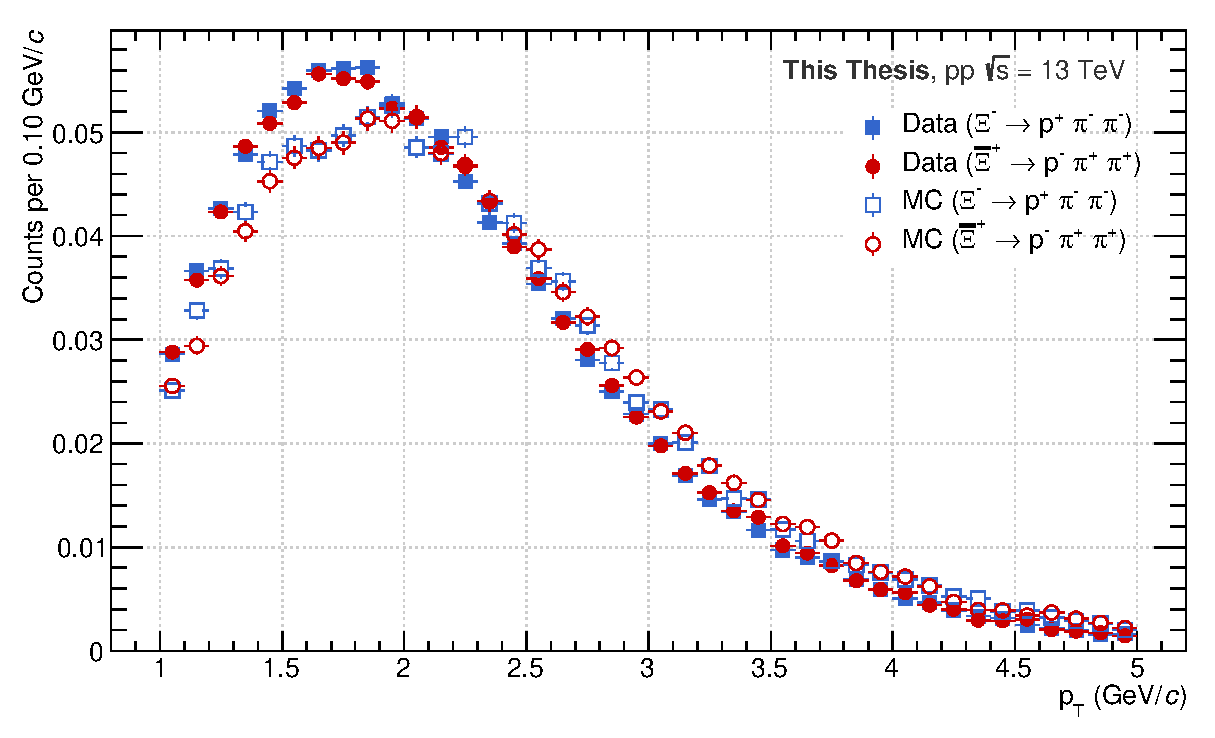
\includegraphics[width=0.6\textwidth]{Figs/Chapter5/RawPtSpectra_Xi.eps}
	\label{fig:PtSpectraXi}
} 
\subfigure[]{
	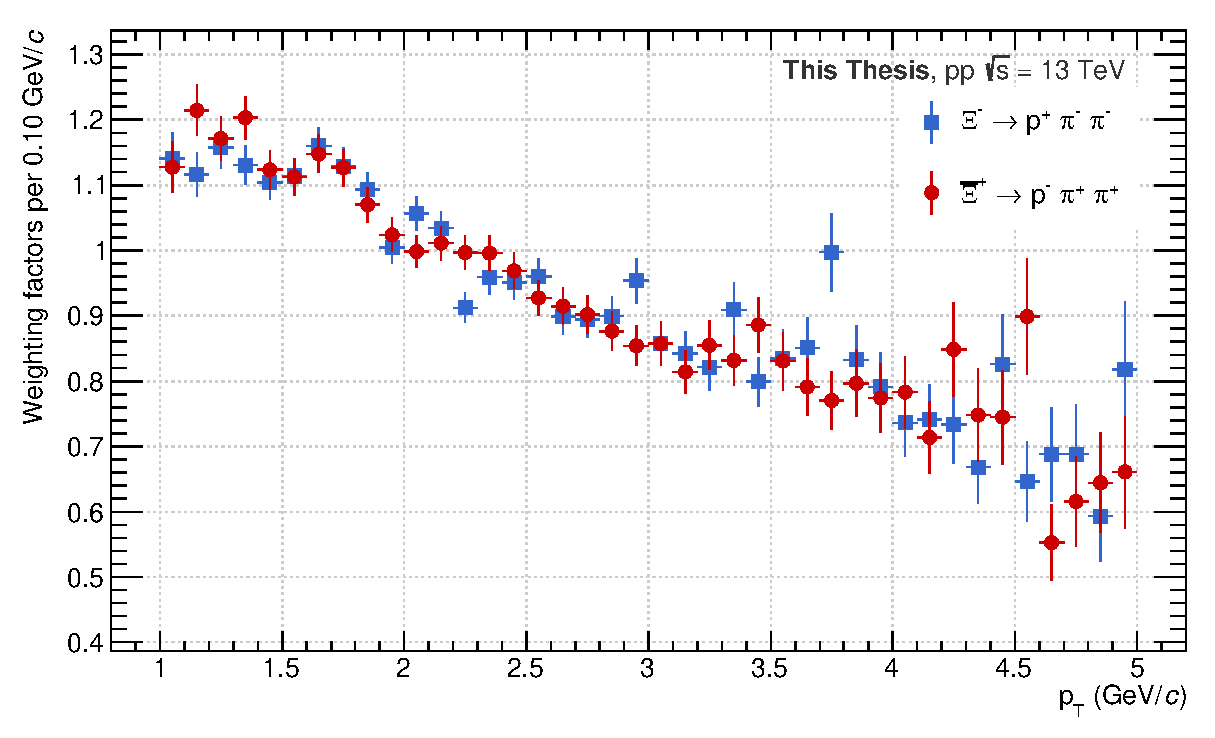
\includegraphics[width=0.6\textwidth]{Figs/Chapter5/WeightingFactors_Xi.eps}
	\label{fig:WeightFactorsXi}
} 
\hspace*{-1.5cm}
\subfigure[]{
	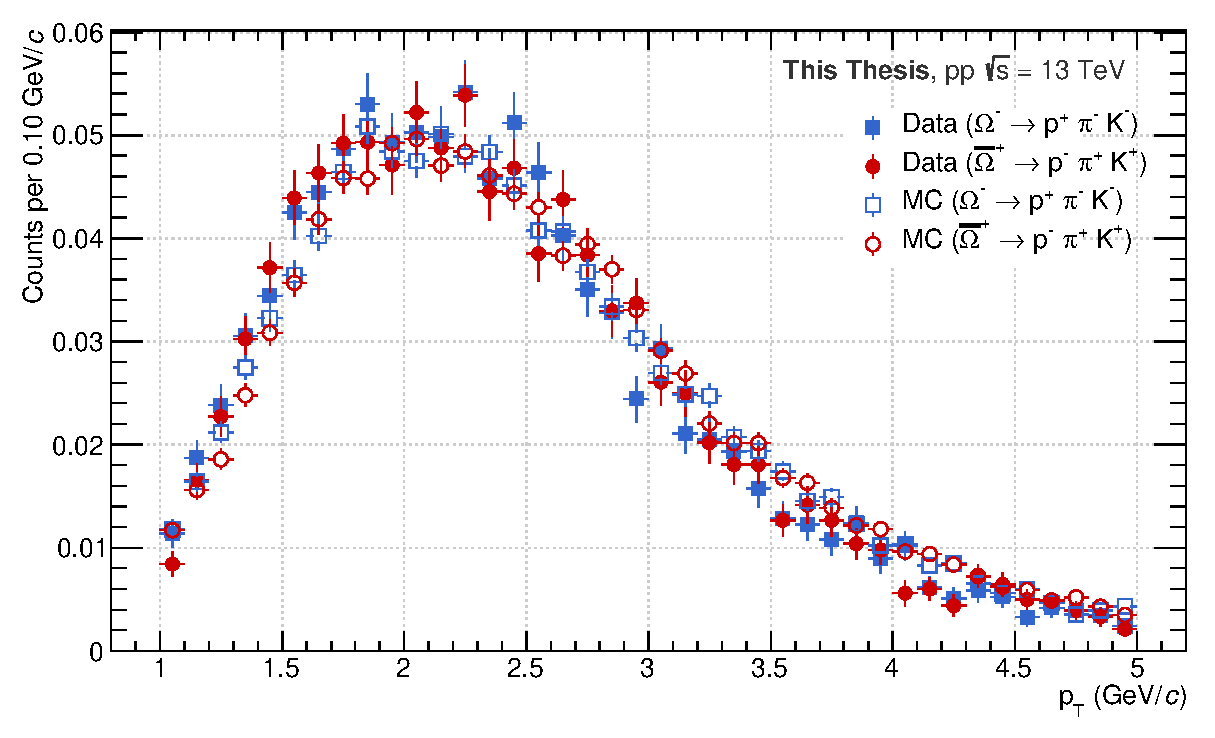
\includegraphics[width=0.6\textwidth]{Figs/Chapter5/RawPtSpectra_Omega.eps}
	\label{fig:PtSpectraOmega}
} 
\subfigure[]{
	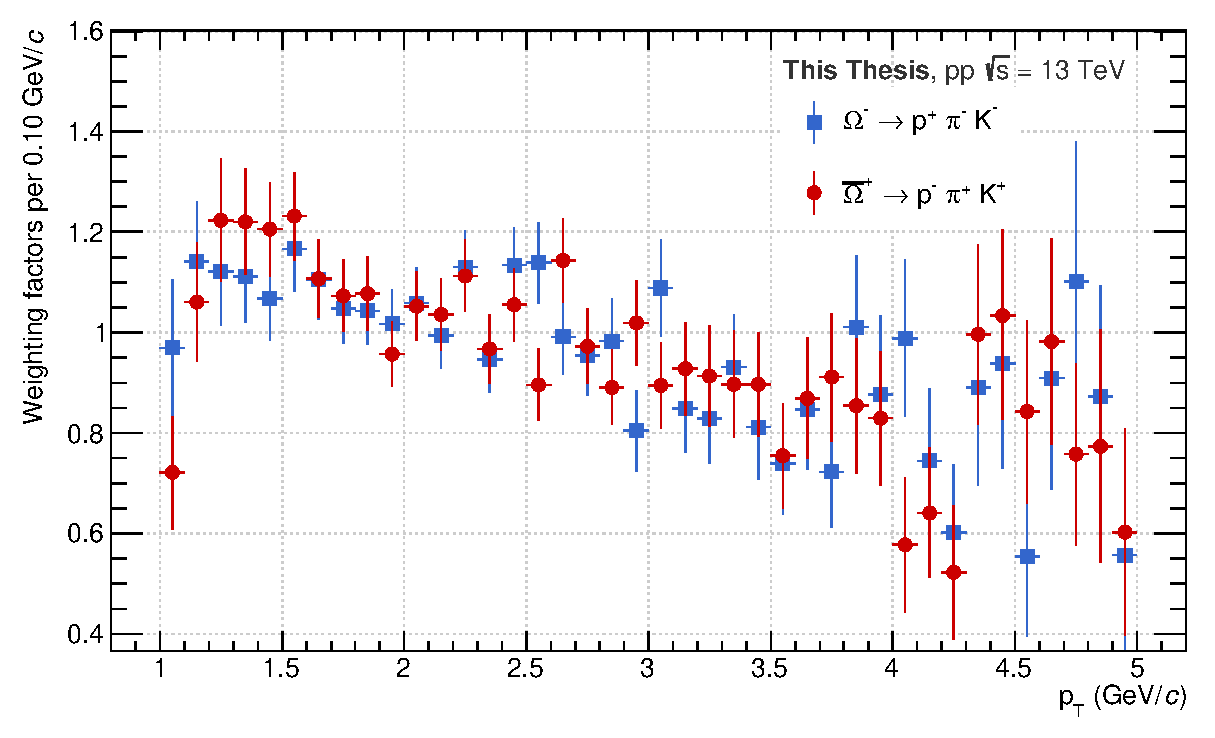
\includegraphics[width=0.6\textwidth]{Figs/Chapter5/WeightingFactors_Omega.eps}
	\label{fig:WeightFactorsOmega}
}  
\caption{On the left: raw \pT spectra of \rmXiM and \rmAxiP (a), and \rmOmegaM and \rmAomegaP (c) hyperons in the data in full marker, and in simulations in open markers. On the right: weighting factors for \rmXiPM (b) and \rmOmegaPM (d), employed to match the \pT spectra in the data and MC. The error bars encompass only the statistical uncertainties.}
	\label{fig:PtSpectra}
\end{figure}


Once the simulated data have been re-weighted, the mass offset observed in MC with respect to the injected mass is assessed, corrected and taken into account in the mass measurement in real data. \Tab\ref{tab:MCMassOffset} presents these corrections as well as the corrected mass values, \ie those measured in real data after correction of the initial offset in MC. From these derive the (relative) mass difference between particle and anti-particle, given by
\begin{equation}
\frac{\Delta \mu}{\mu}=  2 \cdot \frac{\mu_{\textsc{part.}}-\mu_{\overline{\textsc{part.}}}}{\mu_{\textsc{part.}}+\mu_{\overline{\textsc{part.}}}}.
\label{eq:MassDifference}
\end{equation}
Its (statistical) uncertainty is obtained via propagation of the ones on the mass values, assuming there is no correlation between the particle and anti-particle measurements -- \textit{a priori} correct, since $\mu_{\textsc{part.}}$ and $\mu_{\overline{\textsc{part.}}}$ have been extracted independently\footnote{The facts that i) the particle and anti-particle do not share the same data sample\break (see \Sec\ref{subsubsec:PrinciplesOfMassExtraction}), and ii) the fitting procedure is run separately guarantee the independence of the mass measurements.}--,
\begin{equation}
\sigma_{\Delta \mu /\mu }=  4 \cdot \sqrt{ \left(\frac{-\mu_{\overline{\textsc{part.}}}}{\left(\mu_{\textsc{part.}} + \mu_{\overline{\textsc{part.}}} \right)^{2}}\right)^{2} \sigma_{\mu_{\textsc{part.}}}^{2} + \left(\frac{\mu_{\textsc{part.}}}{\left(\mu_{\textsc{part.}} + \mu_{\overline{\textsc{part.}}} \right)^{2}}\right)^{2} \sigma_{\mu_{\overline{\textsc{part.}}}}^{2} }.
\label{eq:MassDifferenceUncertainty}
\end{equation}
\Tab\ref{tab:MCMassDiffOffset} shows the mass difference for \rmXi and \rmOmega, in the data and MC, as well as the corrected value.

\begin{table}[!t]
    \centering
    \footnotesize
    \begin{tabular}{>{\raggedleft\arraybackslash}b{2.5cm}@{\hspace{0.5cm}} >{\raggedleft\arraybackslash}b{2.5cm}@{\hspace{0.5cm}} >{\raggedleft\arraybackslash}b{2.5cm}@{\hspace{0.5cm}} >{\raggedleft\arraybackslash}b{2.5cm}@{\hspace{0.5cm}} >{\raggedleft\arraybackslash}b{2.5cm}@{\hspace{0.5cm}}}
    \noalign{\smallskip}\hline\noalign{\smallskip}
    \bf Particle & \bf \rmXiM & \bf \rmAxiP & \bf \rmOmegaM & \bf \rmAomegaP \\
    \noalign{\smallskip}\hline \noalign{\smallskip}
    \multicolumn{5}{l}{(In \mmass)} \\
    Offset in data & $0.215 \pm 0.002$  & $0.267\pm 0.002$ & $0.139\pm 0.008$ & $0.123 \pm 0.008$ \\
    Offset in MC & $-0.075 \pm 0.003$  & $-0.072\pm 0.003$ & $0.040\pm 0.005$ & $0.027 \pm 0.005$ \\
    	Corrected mass & $1322.000 \pm 0.003$ & $1322.049 \pm 0.005$ & $1672.549 \pm 0.008$ & $1672.546 \pm 0.008$\\
    \noalign{\smallskip}\hline\noalign{\smallskip}
    \end{tabular}
    \caption{Measurements of the mass offset (the difference between the reconstructed and injected masses) with respect to the PDG value (coinciding with the injected mass in MC) in the data and MC, as well as the final masses of $\Xi^{-}$, $\overline{\Xi}^{+}$, $\Omega^{-}$, $\overline{\Omega}^{+}$ after correction of that offset in MC. The uncertainties on the mass values correspond only to the statistical ones. These measurements have been obtained using the selections in \tab\ref{tab:CascadeSelections}, a triple Gaussian for the peak modelisation and a linear function for the background (in the data only).}\label{tab:MCMassOffset}
\end{table}

\begin{table}[!t]
    \centering
%    \footnotesize
    \begin{tabular}{b{7.5cm}@{\hspace{0.5cm}} b{3cm}@{\hspace{0.5cm}} b{3cm}@{\hspace{0.5cm}}}
    	\noalign{\smallskip}\hline \noalign{\smallskip}    
    \bf Particle & \bf \rmXi & \bf \rmOmega\\
    \noalign{\smallskip}\hline \noalign{\smallskip}  
    Mass difference offset in data ($\times 10^{-5}$) & $3.94 \pm 0.22$  & $-0.97 \pm 0.68$ \\
    Mass difference offset in MC ($\times 10^{-5}$)& $-0.23 \pm 0.33$ & $-0.78 \pm 0.43$  \\
    	Corrected mass difference ($\times 10^{-5}$) & $3.71 \pm 0.22$ & $-0.18 \pm 0.68$ \\
    
    \noalign{\smallskip}\hline\noalign{\smallskip}
    \end{tabular}
    \caption{Measurements of the mass difference in the data and MC, as well as the final mass difference for $\Xi^{\pm}$ and $\Omega^{\pm}$ using the corrected mass values in \tab\ref{tab:MCMassOffset}. The uncertainties on the mass differences correspond only to the statistical ones. These measurements have been obtained using the selections in \tab\ref{tab:CascadeSelections}, a triple Gaussian for the peak modelisation and a linear function for the background (in the data only).} 
    \label{tab:MCMassDiffOffset}
\end{table}

\section{Study of the systematic effects}
\label{sec:SystStudy}

A study of the systematic effects -- also called \textit{systematic study} in the particle physicist's jargon -- consists in reviewing an analysis via the test of its different elements. As its name suggests, it involves identifying the sources of systematic uncertainties that might affect the values of the extracted mass and their corresponding uncertainties. Usually, this is achieved by repeating the analysis with a few \say{minor} changes, hoping that no effect will be observed in the results. In such case, meaning that the obtained values are consistent, then one could argue that the analysis is free of systematic effect and under control: no additional measure are requested. On the contrary, a significant deviation in the analysis results indicates the presence of a systematic effect, that should be treated seriously. 

In practice, one needs to define what \say{small} and \say{large} deviations mean. If an analysis is performed in two different ways: the first approach gives the result $a_1$ with an uncertainty $\sigma_1$ ; the second $a_2$ with an uncertainty $\sigma_2$. The difference between the results is given by $\Delta = a_1 - a_2$ and the error on the difference by\footnote{The formula given here corresponds in fact to the case where two measurements are done of a set and subset of the same dataset, which is typically the case here, unless specificied otherwise.} $\sigma_{\Delta} = \sqrt{ |\sigma_{1}^{2} - \sigma_{2}^{2} | }$. If the ratio $\Delta/\sigma_{\Delta}$ is greater than a certain threshold value -- denoted \sigmaBarlow and to be defined by the analyser --, this points out a systematic effect that requires further investigation. This approach is known as the \textit{Barlow criterion}.

As in cooking, what separates the good systematic study from the lesser good one is the choice of the seasoning, namely the choice of the threshold value. The larger the \sigmaBarlow, the more systematic effects would slip under the radar; conversely, the smaller the threshold, the higher the sensitivity to the systematic effects. Since the targeted precision on the mass and mass difference values is very low, the systematic effects must be well under control. Therefore, in the context of this analysis, the contribution of a potential source of systematics is said to be significant for $\sigmaBarlow\simeq 1$. \\

However, the presence of a systematic effect does not necessarily imply a systematic uncertainty. In fact, there are two possibilites. Either a systematic correction can be applied and the error on that correction will be quoted as the systematic uncertainty, or the correction may be difficult (or impossible) to derive and therefore the systematic uncertainty will have to fully encompass the imprecision induced to the systematic effect.

This treatement of the systematic biases corresponds to the one proposed by Roger Barlow \cite{barlowSLUOLecturesStatistics2000}\cite{barlowSystematicErrorsFacts2002}. The following section presents the list of systematic sources studied for this analysis, with their estimated uncertainties or corrections.

\subsection{Topological and track selections}
\label{subsec:SystTopoAndTrackSelections}

\subsubsection{Influence on the mass extraction}
\label{subsubsec:SystTopoMass}

As explained in \Sec\ref{subsec:TopoReco}, the identification of the charged \rmXi and \rmOmega baryons relies on their characteristic cascade decay. The reconstruction of this decay topology revolves around, first, the association of two tracks to form \rmLambda candidates, and then these are matched with the remaining secondary tracks. In order to reduce the induced combinatorial background, various topological and kinematic cuts are used. The choice of the employed cut values may obviously be the source of a bias. Such a systematic effect can be revealed by observing how a different set of selections affects the mass and its uncertainty.\\

The standard approach consists in varying individually each selection, while keeping the others at their reference value. Although it allows to address the bias induced by a given cut, this does not take into account the possible correlations between topological variables. For instance, a higher cut on cascade decay radius also implies that the \rmLambda daughter decays further away in the detector. To tackle that, one would need to build a matrix containing the correlation factors for each pair of selection variables. Since the cascade identification relies here on a set of seventeen selections, this boils down to determining a symmetric matrix of dimension $15 \times 15$.

\begin{table}[t]
    \hspace*{-1.cm}
    \begin{tabular}{c|c|c}
    \noalign{\smallskip}\hline \noalign{\smallskip}
    \bf Track variable & Variation range & Signal variation \rmXiM (\rmAxiP) \\
    \noalign{\smallskip}\hline \noalign{\smallskip}
    Nbr of crossed TPC readout rows & $> \left[ 70 ; 90 \right]$ &  1\% (1\%)\\
    $\Nsigma^{\rm TPC}$ & $<\left[ 1 ; 3 \right] $ &  60\% (60\%)\\
    
    \noalign{\smallskip}\hline \noalign{\smallskip}
    \bf Topological variable & Variation range & Signal variation \rmXiM (\rmAxiP) \\
    \noalign{\smallskip}\hline \noalign{\smallskip}
    
    \multicolumn{3}{l}{\textbf{V0}} \\
    V0 decay radius (\cm) & $> \left[ 1.2 ; 8 \right]$ & 11\% (11\%)\\
    V0 cosine of pointing angle & $> \left[ 0.97 ; 0.998 \right]$ & 10\% (10\%)\\
    |$m$(V0) - \mPDG[\rmLambda]| (\gmass) & $< \left[ 0.002 ; 0.007 \right]$ & 18\% (18\%)\\
    DCA proton to prim. vtx (\cm) &  $> \left[ 0.04 ; 0.5 \right]$ & 28\% (28\%)\\
    DCA pion to prim. vtx (\cm) &  $> \left[ 0.04 ; 0.95 \right]$ & 10\% (10\%)\\
    DCA V0 to prim. vtx (\cm) & $> \left[ 0.06 ; 0.2 \right]$ & 12\% (12\%)\\
    DCA between V0 daughters (std dev) & $< \left[ 0.4 ; 1.2 \right]$ & 12\% (12\%) \\
    \noalign{\smallskip}\hline \noalign{\smallskip}
    
    \multicolumn{3}{l}{\textbf{Cascade}} \\
    Cascade decay radius (\cm) & $> \left[ 0.5 ; 2.5 \right]$ & 11\% (11\%)\\
    Cascade Lifetime (\cm) & $< \left[ 1.6 ; 3.40 \right]$ \cTau & 40\% (40\%)\\
    DCA bachelor to prim. vtx (\cm) & $> \left[ 0.04 ; 0.5 \right]$ & 15\% (15\%) \\
    DCA between the cascade daughters (std dev) &  $< \left[ 0.25 ; 1.2 \right]$ & 12\% (12\%)\\
    Cascade cosine of pointing angle & $> \left[ 0.995 ; 0.9995 \right]$ & 14\% (14\%)\\
    Bachelor-proton pointing angle (rad) & $> \left[ 0.02 ; 0.05 \right]$ & 11\% (11\%) \\
    
    \noalign{\smallskip}\hline \noalign{\smallskip}
    \end{tabular}
    \caption{Summary of the variation ranges on the topological and track selections employed in the \rmXiM and \rmAxiP reconstruction. The last column indicates the \textit{maximum} induced signal variation; for more details, look at \fig\ref{fig:SignalVariation_TopoSel_XiMinus} and \fig\ref{fig:SignalVariation_TopoSel_XiPlus}.}\label{tab:SystematicSelectionsXi}
\end{table}

However, a different approach is followed here. To go over the correlations between each variable, the sets of selections are randomly generated according to uniform laws\footnote{An alternative approach has also been tried along the \say{natural} distribution of each selection variable, rather than the uniform distribution. In the end, both approaches yield to consistent systematic uncertainties (within a few \kmass). The extra complexity and CPU cost of the alternative way have weighed in, given the fact that the randomisations here are part and parcel of the default analysis flow (see later), and will be resorted to many times. Therefore, the uniform randomisation has been retained as default option for all what is coming next.}, that spans over a certain variation ranges. The critical point of this study resides in the choice of the variation ranges, where a careful balance must be found: it should not be too \say{severe} at the risk of losing all the signal, or too \say{gentle} to cause any significant shift. It is considered as satisfactory when the induced signal shift reaches approximately, at least, 10\%\footnote{Note that this condition is applied for each topological cuts. For other selections, it may be difficult to satisfy such criterion as they act on the background rather than the signal. This is the case, for example, with the competing mass rejection that could never reach the 10\% signal variation threshold, even with an excessively vast range of variation.}. \Tabs\ref{tab:SystematicSelectionsXi} and \ref{tab:SystematicSelectionsOmega}, list the considered selection variables, with their variation range as well as the induced signal variation\footnote{The signal variations have been estimated by varying each selection individually, while keeping all other selections to their values in \tab\ref{tab:CascadeSelections}.} for \rmXi and \rmOmega respectively. As for the \rmKzeroS and \rmLambda, this is summarised in \tabs\ref{tab:SystematicSelectionsK0s} and \ref{tab:SystematicSelectionsLambda}. \\

\begin{table}[t]
    \hspace*{-1.cm}
    \begin{tabular}{c|c|c}
    \noalign{\smallskip}\hline \noalign{\smallskip}
    \bf Candidate variable & Range & Signal variation \rmOmegaM (\rmAomegaP) \\
    \noalign{\smallskip}\hline \noalign{\smallskip}    
    Competing mass rejection (\gmass) & $> \left[ 0.006 ; 0.010 \right]$ & 0.9\% (0.9\%)\\
    
    \noalign{\smallskip}\hline \noalign{\smallskip}
    \bf Track variable & Range & Signal variation \rmOmegaM (\rmAomegaP) \\
    \noalign{\smallskip}\hline \noalign{\smallskip}
    Nbr of crossed TPC readout rows & $> \left[ 70 ; 90 \right]$ &  2.5\% (2.5\%)\\
    $\Nsigma^{\rm TPC}$ & $< \left[ 1 ; 3 \right] $ &  60\% (60\%)\\
    
    \noalign{\smallskip}\hline \noalign{\smallskip}
    \bf Topological variable & Range & Signal variation \rmOmegaM (\rmAomegaP) \\
    \noalign{\smallskip}\hline \noalign{\smallskip}
    
    \multicolumn{3}{l}{\textbf{V0}} \\
    V0 decay radius (\cm) & $> \left[ 1 ; 5.5 \right]$ & 11\% (11\%)\\
    V0 cosine of pointing angle & $> \left[ 0.97 ; 0.998 \right]$ & 17\% (17\%)\\
    |$m$(V0) - \mPDG[\rmLambda]| (\gmass) & $< \left[ 0.002 ; 0.007 \right]$ & 17\% (17\%)\\
    DCA proton to prim. vtx (\cm) & $> \left[ 0.04 ; 0.5 \right]$ & 34\% (34\%)\\
    DCA pion to prim. vtx (\cm) & $> \left[ 0.04 ; 0.75 \right]$ & 10\% (10\%) \\
    DCA V0 to prim. vtx (\cm) & $> \left[ 0.06 ; 0.2 \right]$ & 14\% (14\%)\\
    DCA between V0 daughters (std dev) & $< \left[ 0.4 ; 1.2 \right]$ & 11\% (11\%)\\
    \noalign{\smallskip}\hline \noalign{\smallskip}
    
    \multicolumn{3}{l}{\textbf{Cascade}} \\
    Cascade decay radius (\cm) & $> \left[ 0.5 ; 1.6 \right]$ & 12\% (12\%)\\
    Cascade Lifetime (\cm) & $< \left[ 1.6 ; 3.40 \right]$ \cTau & 14\% (14\%)\\
    DCA bachelor to prim. vtx (\cm) & $> \left[ 0.05 ; 0.2 \right]$ & 13\% (13\%)\\
    DCA between the cascade daughters (std dev) & $< \left[ 0.15 ; 1.2 \right]$ & 12\% (12\%)\\
    Cascade cosine of pointing angle & $> \left[ 0.995 ; 0.9995 \right]$ & 17\% (17\%)\\
    Bachelor-proton pointing angle & $> \left[ 0.02 ; 0.05 \right]$ & 13\% (13\%)\\
    
    \noalign{\smallskip}\hline \noalign{\smallskip}
    \end{tabular}
    \caption{Summary of the variation ranges on the topological and track selections employed in the \rmOmegaM and \rmAomegaP reconstruction. The last column indicates the \textit{maximum} induced signal variation; for more details, look at \fig\ref{fig:SignalVariation_TopoSel_OmegaMinus} and \fig\ref{fig:SignalVariation_TopoSel_OmegaPlus}.}\label{tab:SystematicSelectionsOmega}
\end{table}

The analysis is repeated for each randomly generated set of cuts $i$, as detailed in \Sec\ref{subsec:MassExtraction}, meaning that a mass $\mu_{i}$ and its uncertainty $\sigma_{i}$ are extracted from the fit of the corresponding invariant mass distribution in the data and MC. However, only the values passing the following criteria are retained:

\begin{itemize}
\item[$\bullet$] the fitting procedure must have converged;
\item[$\bullet$] to ensure a good fit quality, its reduced $\chi^{2}$ needs to be relatively close to the unity, $\rmChiSquareNDF < 3$;
\item[$\bullet$] the uncertainties on the mass value are expected to be below the \mmass. Since the \rmXi and \rmOmega masses are of the order of \gmass, a $\sigma_{\mu_{i}}$ at the level of 0.1\% of $\mu_{i}$ represents an uncertainty greater than 1 \mmass. In order to remove outliers, it is required that $\sigma_{\mu_{i}}/\mu_{i} < 0.1\%$.
\end{itemize}

Under these conditions and over a sufficiently large number of sets of cuts, the distributions $\mu_{i}$ and $\sigma_{\mu_{i}}$ can be built. These offer the opportunity to re-qualify the mass and its uncertainties, \ie what will become the default strategy for this analysis outcome:
\begin{itemize}
\item[$\bullet$] the \textit{measured mass} corresponds to the mean value of the $\mu_{i}$ distribution,
\item[$\bullet$] the \textit{systematic uncertainty} due to the candidate selections is the standard deviation of the $\mu_{i}$ distribution,
\item[$\bullet$] and the \textit{statistical uncertainty} is given by the mean value of the $\sigma_{\mu_{i}}$ distribution.
\end{itemize}
As opposed to most analyses, this re-definition allows to circumvent the dependence on a reference set of cuts, making the analysis \textit{in principle} more robust.\\

\begin{figure}[!p]
%\centering
\hspace*{-1.5cm}
\subfigure[]{
	\includegraphics[width=0.6\textwidth]{Figs/Chapter5/MassVsNbrOfCutSets\_Xi.eps}
	\label{fig:MassVsNbrOfCutSetsXi}
} 
\subfigure[]{
	\includegraphics[width=0.6\textwidth]{Figs/Chapter5/MassVsNbrOfCutSets\_Omega.eps}
	\label{fig:MassVsNbrOfCutSetsOmega}
} 
\hspace*{-1.5cm}
\subfigure[]{
	\includegraphics[width=0.6\textwidth]{Figs/Chapter5/StatErrVsNbrOfCutSets\_Xi.eps}
	\label{fig:StatErrVsNbrOfCutSetsXi}
} 
\subfigure[]{
	\includegraphics[width=0.6\textwidth]{Figs/Chapter5/StatErrVsNbrOfCutSets\_Omega.eps}
	\label{fig:StatErrVsNbrOfCutSetsOmega}
} 
\hspace*{-1.5cm}
\subfigure[]{
	\includegraphics[width=0.6\textwidth]{Figs/Chapter5/SystErrVsNbrOfCutSets\_Xi.eps}
	\label{fig:SystErrVsNbrOfCutSetsXi}
} 
\subfigure[]{
	\includegraphics[width=0.6\textwidth]{Figs/Chapter5/SystErrVsNbrOfCutSets\_Omega.eps}
	\label{fig:SystErrVsNbrOfCutSetsOmega}
}  
\caption{Relative measured mass as well as its statistical and systematic uncertainties in pp collisions at \sqrtS = 13 \tev as a function of the number of cut sets, for \rmXi in (a), (c), (e) and \rmOmega in (b), (d), (f) respectively. The quantities on the y-axis are relative to the value taken as the final measurement. In this case, it corresponds to the quantity for 20 000 different sets of cuts. Here, the peak is modeled by a modified Gaussian, and the background by a first order polynomial. The error bars represent the uncertainty on the evaluation of the mean or standard deviation.}
	\label{fig:MassVsNentries}
\end{figure}
%\clearpage

The above quantities being extracted from a finite sample, one could expect them to depend on the number of cut sets. The stability of the results with the amount of sets employed has been studied and is shown on \fig\ref{fig:MassVsNentries}. At first, the mass value, its statistical and systematic uncertainties fluctuate with the number of cut sets, until they reach a plateau region at approximately 5000-6000 different sets of cuts. Such amount should thus suffice to perform the mass measurement. However, in order to a guarantee an excellent stability, 20 000 sets are being used.

The output results of this procedure are presented in \tab\ref{tab:SystTopoKineSelections}.

\begin{table}[h]
    \hspace*{-0.4cm}
    \begin{tabular}{cccc|ccc}

%    \begin{tabular}{b{2cm}@{\hspace{0.5cm}} b{3cm}@{\hspace{0.5cm}} b{2cm}@{\hspace{0.5cm}} b{2cm}@{\hspace{0.5cm}} b{5cm}@{\hspace{0.5cm}} b{3cm}@{\hspace{0.5cm}} b{3cm}@{\hspace{0.5cm}}}
    \noalign{\smallskip}\hline \noalign{\smallskip}
    \bf Particle & \bf Measured & \multicolumn{2}{c|}{\bf Uncertainty} & \bf Measured & \multicolumn{2}{c}{\bf Uncertainty}\\
    & \bf mass & \bf stat. & \bf syst. & \bf mass difference & \bf stat. & \bf syst.\\
    & (\mmass) & (\mmass) & (\mmass) & ($\times 10^{-5}$) & ($\times 10^{-5}$) & ($\times 10^{-5}$) \\
    \noalign{\smallskip}\hline \noalign{\smallskip}
    \rmKzeroS & 497.737 & 0.003 & 0.010 & / & / & / \\
	\noalign{\smallskip}\hline \noalign{\smallskip}
    \rmLambda & 1115.618 & 0.002 & 0.011 & \multirow{2}{*}{4.78} & \multirow{2}{*}{0.17} & \multirow{2}{*}{0.14} \\
	\rmAlambda & 1115.671 & 0.002 & 0.012 & & & \\
    \noalign{\smallskip}\hline \noalign{\smallskip}
    \rmXiM & 1321.728 & 0.004 & 0.016 & \multirow{2}{*}{3.95} & \multirow{2}{*}{0.37} & \multirow{2}{*}{0.39} \\
	\rmAxiP & 1321.780 & 0.004 & 0.019 & & & \\
    \noalign{\smallskip}\hline \noalign{\smallskip}
    \rmOmegaM & 1672.536 & 0.014 & 0.015 & \multirow{2}{*}{-1.31} & \multirow{2}{*}{1.14} & \multirow{2}{*}{0.76} \\ 
    \rmAomegaP &  1672.514 & 0.014 & 0.015 & & & \\ 
	\noalign{\smallskip}\hline \noalign{\smallskip}
    \end{tabular}
    \caption{Measured masses and mass differences of \rmKzeroS, \rmLambda, \rmXi and \rmOmega, accompanied by their statistical and systematic (due to the topological and kinematic selections) uncertainties. Here, the measurements have been performed with a triple Gaussian for the signal and a first order polynomial for the background.}\label{tab:SystTopoKineSelections}
\end{table}

\subsubsection{Influence on the mass difference mass}

In \tab\ref{tab:SystTopoKineSelections}, the mass difference have been obtained taking the independently measured mass values of the particle and the anti-particle from the above procedure (\Sec\ref{subsubsec:SystTopoMass}), and using \eq\ref{eq:MassDifference}. The uncertainties are then propagated to obtain the statistical and systematic uncertainties on the mass difference. It does not result directly from the aforementioned procedure. In that sense, the mass difference measurement is \textit{indirect}. It carries the full systematic uncertainties from the particle and anti-particle mass values. By extracting the mass difference in a more \textit{direct} way -- similarly to what is done for the mass in \Sec\ref{subsubsec:SystTopoMass} --, part of the uncertainties from the particle and anti-particle masses would cancel out in the difference, resulting in a smaller systematic uncertainty.\\

To that end, an additional step needs to be introduced in the previous strategy in \Sec\ref{subsubsec:SystTopoMass}. For each set of cuts $i$, both particle and anti-particle masses -- $\mu_{i, \textsc{part.}}$ and $\mu_{i, \overline{\textsc{part.}}}$ --  are extracted as well as their uncertainties, $\sigma_{i, \textsc{part.}}$ and $\sigma_{i, \overline{\textsc{part.}}}$. From these, the computation of the mass difference is performed, 
\begin{equation}
\frac{\Delta \mu_{i}}{  \mu_{i} } = 2 \cdot \frac{\mu_{i, \textsc{part.}}-\mu_{i, \overline{\textsc{part.}}}}{\mu_{i, \textsc{part.}}+\mu_{i, \overline{\textsc{part.}}}},
\end{equation}
and the uncertainties are propagated in order to get the one on the mass difference, 
\begin{equation}
\sigma_{\Delta \mu_{i} /\mu_{i} }=  4 \cdot \sqrt{ \left(\frac{-\mu_{i, \overline{\textsc{part.}}}}{\left(\mu_{i, \textsc{part.}} + \mu_{i, \overline{\textsc{part.}}} \right)^{2}}\right)^{2} \sigma_{\mu_{i, \textsc{part.}}}^{2} + \left(\frac{\mu_{i, \textsc{part.}}}{\left(\mu_{i, \textsc{part.}} + \mu_{i, \overline{\textsc{part.}}} \right)^{2}}\right)^{2} \sigma_{\mu_{i, \overline{\textsc{part.}}}}^{2} }.
\end{equation}\\

Similarly to the mass extraction, the mass difference and its uncertainties are calculated from the $\Delta \mu_{i}/  \mu_{i}$ and $\sigma_{\Delta \mu_{i} /\mu_{i} }$ distributions over $N$ different set of cuts:
\begin{itemize}
\item[$\bullet$] the \textit{measured mass difference} corresponds to the mean value of the $\Delta \mu_{i}/  \mu_{i}$ distribution,
\item[$\bullet$] the \textit{systematic uncertainty} due to the candidate selections is the standard deviation of the $\Delta \mu_{i}/  \mu_{i}$ distribution,
\item[$\bullet$] and the \textit{statistical uncertainty} is given by the mean value of the $\sigma_{\Delta \mu_{i} /\mu_{i} }$ distribution.
\end{itemize}

\begin{table}[t]
    \centering
    \begin{tabular}{cccc}
    \noalign{\smallskip}\hline \noalign{\smallskip}
    Particle & Mass difference & \multicolumn{2}{c}{Uncertainty}\\  
    & ($\times 10^{-5}$) & statistical ($\times 10^{-5}$) & systematic ($\times 10^{-5}$) \\
    \noalign{\smallskip}\hline \noalign{\smallskip}
    \multicolumn{4}{l}{\bf \rmLambda} \\
    Indirect & \bf 4.54 &  0.75 & 1.50 \\
    Direct & \bf 4.68 & 0.77 & 0.79 \\ 
    \noalign{\smallskip}\hline \noalign{\smallskip}
    \multicolumn{4}{l}{\bf \rmXi} \\
    Indirect & \bf 4.54 &  0.75 & 1.50 \\
    Direct & \bf 4.68 & 0.77 & 0.79 \\ 
    \noalign{\smallskip}\hline \noalign{\smallskip}
    \multicolumn{4}{l}{\bf \rmOmega} \\
    Indirect & \bf 0.48 & 1.74 & 1.57  \\
    Direct & \bf 0.53 & 1.75 & 1.19   \\
    \noalign{\smallskip}\hline \noalign{\smallskip}
    \end{tabular}
    \caption{Comparison between \textit{direct} and \textit{indirect} mass difference values of \rmXi and \rmOmega baryons, with their respective uncertainties (statistical and systematical). The total uncertainty is obtained by summing quadratically the statistical and systematical uncertainties. Here, both direct and indirect measurements have been performed with a modified Gaussian for the peak and a first order polynomial for the side-bands.}\label{tab:SystMassDifference}
\end{table}

The results on the directly extracted mass difference are presented in \tab\ref{tab:SystMassDifference}. Although the values obtained directly are consistent with the indirect ones, the associated systematic uncertainties are smaller by approximately 48\% for \rmXi and 25\% for \rmOmega. Due to this gain in precision, from now on, the mass difference will always be extracted \say{directly}.

\subsection{Stability of the results}
\label{subsec:StabilityResults}

All the elements of the analysis being now introduced, it is essential to control the stability of the results. In other words, it consists to adapt and calibrate the analysis, in order to ensure that the presented measurements can be trusted and do not fluctuate over time, space, momentum, etc. This requires a fine and thorough inspection of what happens throughout the data acquisition and reconstruction. If needed, these shall be tuned in such a way, for instance, that the momentum calibration is satisfactory; or at least, one should identify a region in time, space, momentum, etc, where the latter requirement would be fullfilled.

The measurement of the mass \textit{a priori} relies on a countless number of parameters, some of them being possibly correlated. This analysis focuses on seven possible dependencies on the mass. For the sake of brievety, only figures related to one or two particles will be presented in this manuscript.

\subsubsection{Dependence on the data taking periods}
\label{subsubsec:DataTakingDependence}

As mentioned above, an important check involves the stability of the results over time, that is as a function of the data taking periods. \Sec\ref{subsec:DataSamples} specifies that all the pp collisions recorded in the 2016, 2017 and 2018 data taking periods are considered. This corresponds to 37 periods collected in different magnetic field configurations for the L3 solenoid magnet\footnote{For almost all the periods, the L3 solenoid and the dipole magnets share the magnetic field polarity, that is $(+,+)$ or $(-,-)$. Each rule has its exception: one data taking periods in 2018 has been collected with the dipole magnet off.} ($B = + 0.5, -0.5, -0.2$ T), TPC gas composition (Ar/CO$_{2}$ for 2016 and 2018; Ne/CO$_{2}$/N$_{2}$ for 2017), and trigger modes (\say{CENT} or \say{FAST}). They are designated by a tag made of two numbers -- corresponding to the last digits of the data taking year -- and a letter, labelling for the period.

\Figs\ref{fig:MassVsPeriodsXi} and \ref{fig:MassVsPeriodsOmega} show the measured mass of \rmXi and \rmOmega hyperons respectively, as a function of the data sample. A striking feature on these figures is the fact that all the values seem to be systematically off by about 250 \kmass for the double strange baryons and 150 \kmass for the triple strange particles. This originates from a momentum bias occuring in the V0 and cascade reconstruction, which is addressed later in \Sec\ref{subsubsec:DecayRadiusDependence}. Once it is corrected, the mass measurements lie within the PDG uncertainties.

\begin{landscape}
\begin{figure}[p]
\centering
%\hspace*{-1.5cm}
\subfigure[]{
	\includegraphics[width=1.45\textwidth]{Figs/Chapter5/MassVsPeriod2\_Xi.eps}
	\label{fig:MassVsPeriodsXi}
} \\
%\hspace*{-1.5cm}
\subfigure[]{
	\includegraphics[width=1.45\textwidth]{Figs/Chapter5/MassVsPeriod2\_Omega.eps}
	\label{fig:MassVsPeriodsOmega}
} 
\caption{Measured mass of the \rmXiM and \rmAxiP (top), and \rmOmegaM and \rmAomegaP baryons (bottom) as a function of the \textbf{data taking period}. These values have been obtained based on 20 000 different sets of selections (\Sec\ref{subsec:SystTopoAndTrackSelections}). Hence, the uncertainties correspond to the quadratic sum of the statistical and systematic uncertainties due to the candidate and track selections. The periods with a magnetic field of $B = +0.5$~T are indicated with blue circles, those with the opposite polarity are shown in red squares, and finally the data sample collected in a configuration of $B~=~-0.2$~T are represented in black diamonds. Moreover, the "/C" and "/F" tags are here to signify "CENT" and "FAST" trigger modes respectively.}
	\label{fig:MassVsPeriods}
\end{figure}
\end{landscape}

The mass measurements in periods collected with $B =-0.2$~T stand out from the rest of the values. This behaviour is attributed to the lower magnetic field, which results in a deterioration of the momentum resolution. The \say{FAST} configuration -- \ie events collected without the two middle layers of the ITS, the SDDs -- exhibits a similar pattern. The latter is most certainly due to the missing SDD informations; without these constraints, the probability to incorrectly assigned a cluster to a track increases. As a consequence, the track quality in the ITS, as well as the tracking efficiency, drop but also the track momentum gets biased. This point has been cross-checked by repeating the analysis in pp collisions at \sqrtS = 5.02 \tev with $B = \pm 0.5$~T\footnote{For comparison, the exploited data sample of pp collisions at \sqrtS = 13 \tev counts about 2.6 billons minimum-bias events while, for the one at \sqrtS = 5.02 \tev, it amounts to approximately 520 millions minimum-bias events.}, in \say{CENT} and \say{FAST} modes. In the former configuration, the results agreed with those obtained at 13 \tev (for the same magnetic field polarity) whereas, in the latter case, the previous trend was again observed, pointing indeed towards a problem related to the missing SDD informations. Therefore, the data sample taken in a magnetic field of $B = -0.2$ T and/or collected with the \say{FAST} trigger mode are discarded for the rest of the analysis.

Finally, concerning the periods with opposite polarities, the results shows a very good agreement. A fit with a constant function (not shown on the figure) displays a $\chi^2$ probability greater than 90\%.

\subsubsection{Dependence on the decay radius}
\label{subsubsec:DecayRadiusDependence}

A critical aspect of the analysis is to make sure to have a satisfactory calibration of the momentum. A miscalibration of the latter typically originates either from an imprecision on the magnetic field or imperfect energy loss corrections. The former being addressed in \Sec\ref{subsubsec:ImprecisionMagneticField}, this section thus concentrates on the second point.

Miscalculation of the energy losses can arise at two different levels: on one hand, the actual amount of material budget may not be properly accounted for in the detector geometry. In other words, there could be a significant misknowledge on the amount of material budget in the detector. \Sec\ref{subsubsec:ImperfectEnergyLossCorrections} is devoted to this aspect. On the other hand, the calculation of the energy loss corrections could be erroneous. A hint of the latter can be found by looking at the dependence of the measured mass on the decay radius, \fig\ref{fig:MassVsRadius}.\\

\begin{figure}[h]
%\centering
\hspace*{-2.cm}
\subfigure[]{
	\includegraphics[width=0.6\textwidth]{Figs/Chapter5/MassVsRadius\_Xi.eps}
	\label{fig:MassVsRadiusXi}
} 
\subfigure[]{
	\includegraphics[width=0.6\textwidth]{Figs/Chapter5/MassVsRadius\_XiMC.eps}
	\label{fig:MassVsRadiusXiMC}
} 
\hspace*{-2.cm}
\subfigure[]{
	\includegraphics[width=0.6\textwidth]{Figs/Chapter5/MassVsRadius\_Omega.eps}
	\label{fig:MassVsRadiusOmega}
} 
\subfigure[]{
	\includegraphics[width=0.6\textwidth]{Figs/Chapter5/MassVsRadius\_OmegaMC.eps}
	\label{fig:MassVsRadiusOmegaMC}
} 
\caption{Measured mass of the \rmXi (top) and \rmOmega baryons (bottom), in the data (left) and in MC (right), as a function of the \textbf{cascade decay radius}. The average radial position for each ITS layer is indicated with dotted lines. Note that, for the purpose of the comparison, the MC is \textit{not} re-weighted (\Sec\ref{subsubsec:CorrectionOnTheExtractedMass}). In both cases, the results have been obtained through a fit with a triple Gaussian function for the invariant mass peak and, only in the data, an exponential function for the background.}
	\label{fig:MassVsRadius}
\end{figure}

First of all, the measured mass exhibits an unexpected behaviour with the decay radius: it abruptly drops whenever the particle of interest decays in the vicinity of an ITS layer. Furthermore, this trend is well reproduced in simulated data. The \fig\ref{fig:RadiusResolVsRadius} shows the resolution on the cascade decay radius as a function of the radial position. Slighlty above the edge of an ITS detector, this resolution degrades abruptly in such a way that the \rmXi and \rmOmega candidates tend to be reconstructed below the detection layer. This underestimation of decay radius leads to a bias in the energy loss corrections and the opening angle (detailed later in \Sec\ref{subsubsec:OpAngleDependence}), thus lowering the measured mass. For that reason, the regions in the ITS corresponding to these dips will be discarded from now on.\\

\begin{figure}[t]
%\centering
\hspace*{-2.cm}
\subfigure[]{
	\includegraphics[width=0.6\textwidth]{Figs/Chapter5/MassVsRadiusResol\_XiMC.eps}
	\label{fig:RadiusResolVsRadiusXi}
} 
\subfigure[]{
	\includegraphics[width=0.6\textwidth]{Figs/Chapter5/MassVsRadiusResol\_OmegaMC.eps}
	\label{fig:RadiusResolVsRadiusOmega}
} 
\caption{Resolution on the radial position of the \rmXi (top) and \rmOmega (bottom) decay point in MC, as a function of the \textbf{cascade decay radius}. The average radial position for each ITS layer is indicated in dotted line. Here, the MC data have \textit{not} been re-weighted. In both cases, the results have been obtained through a fit with a triple Gaussian function for the invariant mass peak and an exponential function for the background.}
	\label{fig:RadiusResolVsRadius}
\end{figure}

Furthermore, whatever the particle of interest, the measured mass in \fig\ref{fig:MassVsRadius} increases significantly with the decay radius by about 1 \mmass for the \rmXi, in both data and MC. It turns out that this trend results from several approximations in the implementation of the energy loss corrections in the ALICE framework. There are three of them, classified from the most to the \say{least} significant.

\begin{enumerate}
\item As explained in \Sec\ref{subsubsec:TrackReco}, in the final stage of the tracking, all tracks are propagated inwards to their DCA to the primary vertex, taking into account stochastic processes such as energy losses. While this makes sense for primary tracks, it introduces a bias for secondary ones. Being a decay product, the inward propagation of a secondary track should stop at the decay point, where its parameters are related to the mother particle. Instead, at each propagation step between the secondary and primary vertices, the track receives additional energy from \dEdx-corrections (footnote \ref{footnote:EnergyLoss}). This excess of energy builds up with the decay point position, the further away the secondary vertex is, the more biased the track parameters are. Nevertheless, at this stage of the event reconstruction, there is no way to distinguish a primary from a secondary particle\footnote{Concerning V0 decays, there is indeed no way to identify a secondary particle at this stage of the reconstruction using the so-called \textit{offline} reconstruction, presented \chap\ref{chap:V0CascReconstruction}. However, there exists another approach, dubbed \textit{on-the-fly}, that performs the track finding, track fitting and V0 vertexing simultaneously. Although it has been checked that on-the-fly V0s do not exhibit the mass dependence on the radial position of the decay point, they can not be used in the analysis as there exists no on-the-fly cascade.}. For that reason, this bias is expected to be removed later, during the V0 and cascade reconstruction. However, as mentioned in \Sec\ref{subsubsec:V0Formation} (footnote \ref{footnote:EnergyLossV0CascVertexing}), the propagation of daughter tracks from the location of the DCA to the primary vertex to the V0/cascade decay point is performed with no energy loss corrections. This means that the energy previously added during the final inward propagation of the tracking between the secondary and primary vertices, has not been subtracted, leading to additional energy/momentum in the track parameters at the
secondary decay position and thus to an offset in the invariant mass.

\item The energy loss calculation relies on the same parametrisation of the Bethe-Bloch formula (\eq\ref{eq:BetheBloch}) as \GeantThree and \GeantFour\footnote{Although \GeantThree and \GeantFour are two different version of \textsc{Geant} software series, their treatement of the energy losses of a charged particle in a medium remains the same.}. For the parameters related to material, they are using the database in \cite{geant4Geant4MaterialDatabase2022}. However, as explained in \Sec\ref{subsubsec:TrackReco}, the particle energy losses are calculated and corrected assuming that all the materials are made of Si in the ITS volume (including the beam pipe) and Ne in the TPC. This approximation leads inevitably to a systematic misevaluation of the actual energy losses, and thus to bias in the invariant mass.

\begin{figure}[H]
	\centering
	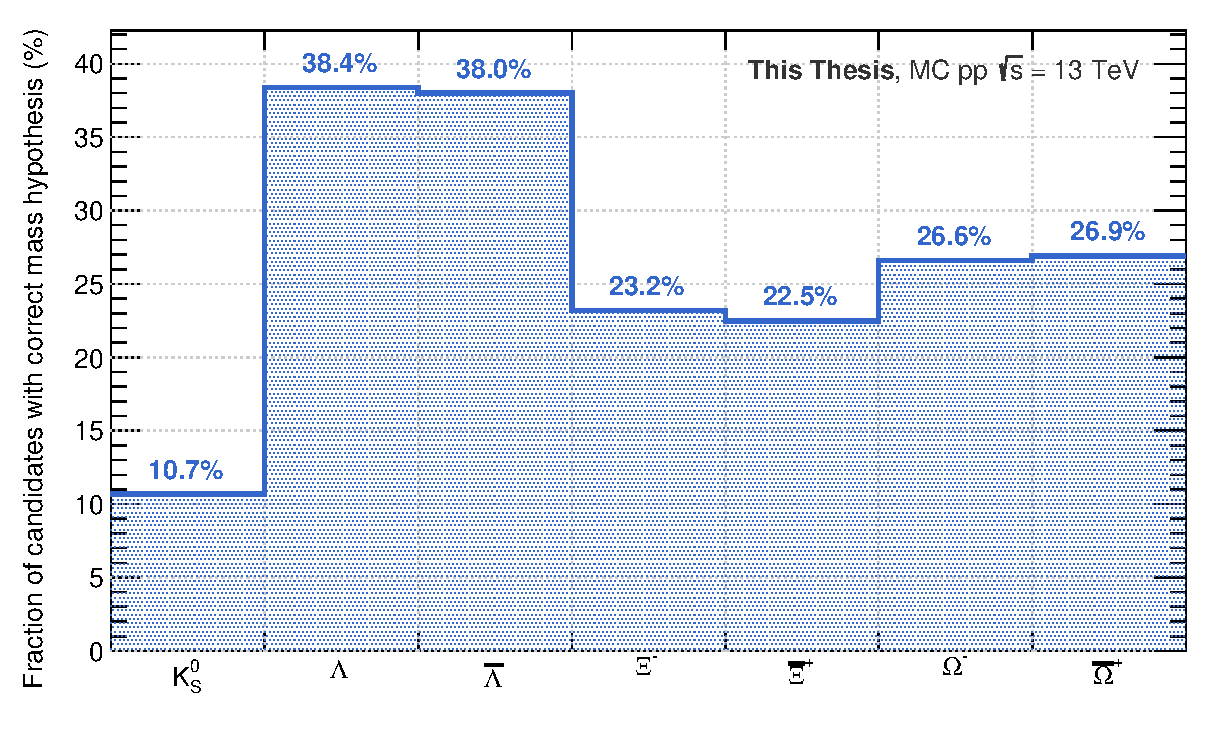
\includegraphics[width=1\textwidth]{Figs/Chapter5/FractionOfPIDForTracking.eps}
	\caption{Fraction of V0 and cascade candidates with the correct mass hypothesis, during the initial track propragation in the event building, for all the associated daughter tracks.}
	\label{fig:FractionOfPIDForTracking}
\end{figure}

\item Along the same line, the Bethe-Bloch formula in \eq\ref{eq:BetheBloch} also depends on the particle traversing the material and, in particular, its charge, momentum and mass. While the Kalman filter provides the first two, the last one comes from the measurement of the energy deposit in the TPC volume, which offers a preliminary particle identification. There is no guarantee, though, that the latter coincides with the expected mass hypothesis  for a \rmKzeroS, \rmLambdaPM, \rmXiPM or \rmOmegaPM decay. For instance, \Sec\ref{subsubsec:TrackReco} explains that the pion mass is taken as default value. As a matter of fact, only a fraction of the candidates has the correct mass hypothesis for both decay daughters as shown in \fig\ref{fig:FractionOfPIDForTracking}. If the mass hypothesis used in the energy loss calculation turns out to be incorrect, the wrong amount of energy loss correction is applied.

\end{enumerate}


There are different ways to address these issues. The approach followed in this analysis consists in i) replaying the track propagation in order to remove the previous energy loss corrections, and ii) re-applying them with the correct mass hypothesis, appropriate material parameters and stopping at the secondary decay position. The \fig\ref{fig:SchemeRetroCorrection} gives a description of this procedure, also called \textit{retro-corrections}.

\begin{figure}[t]
	\centering
	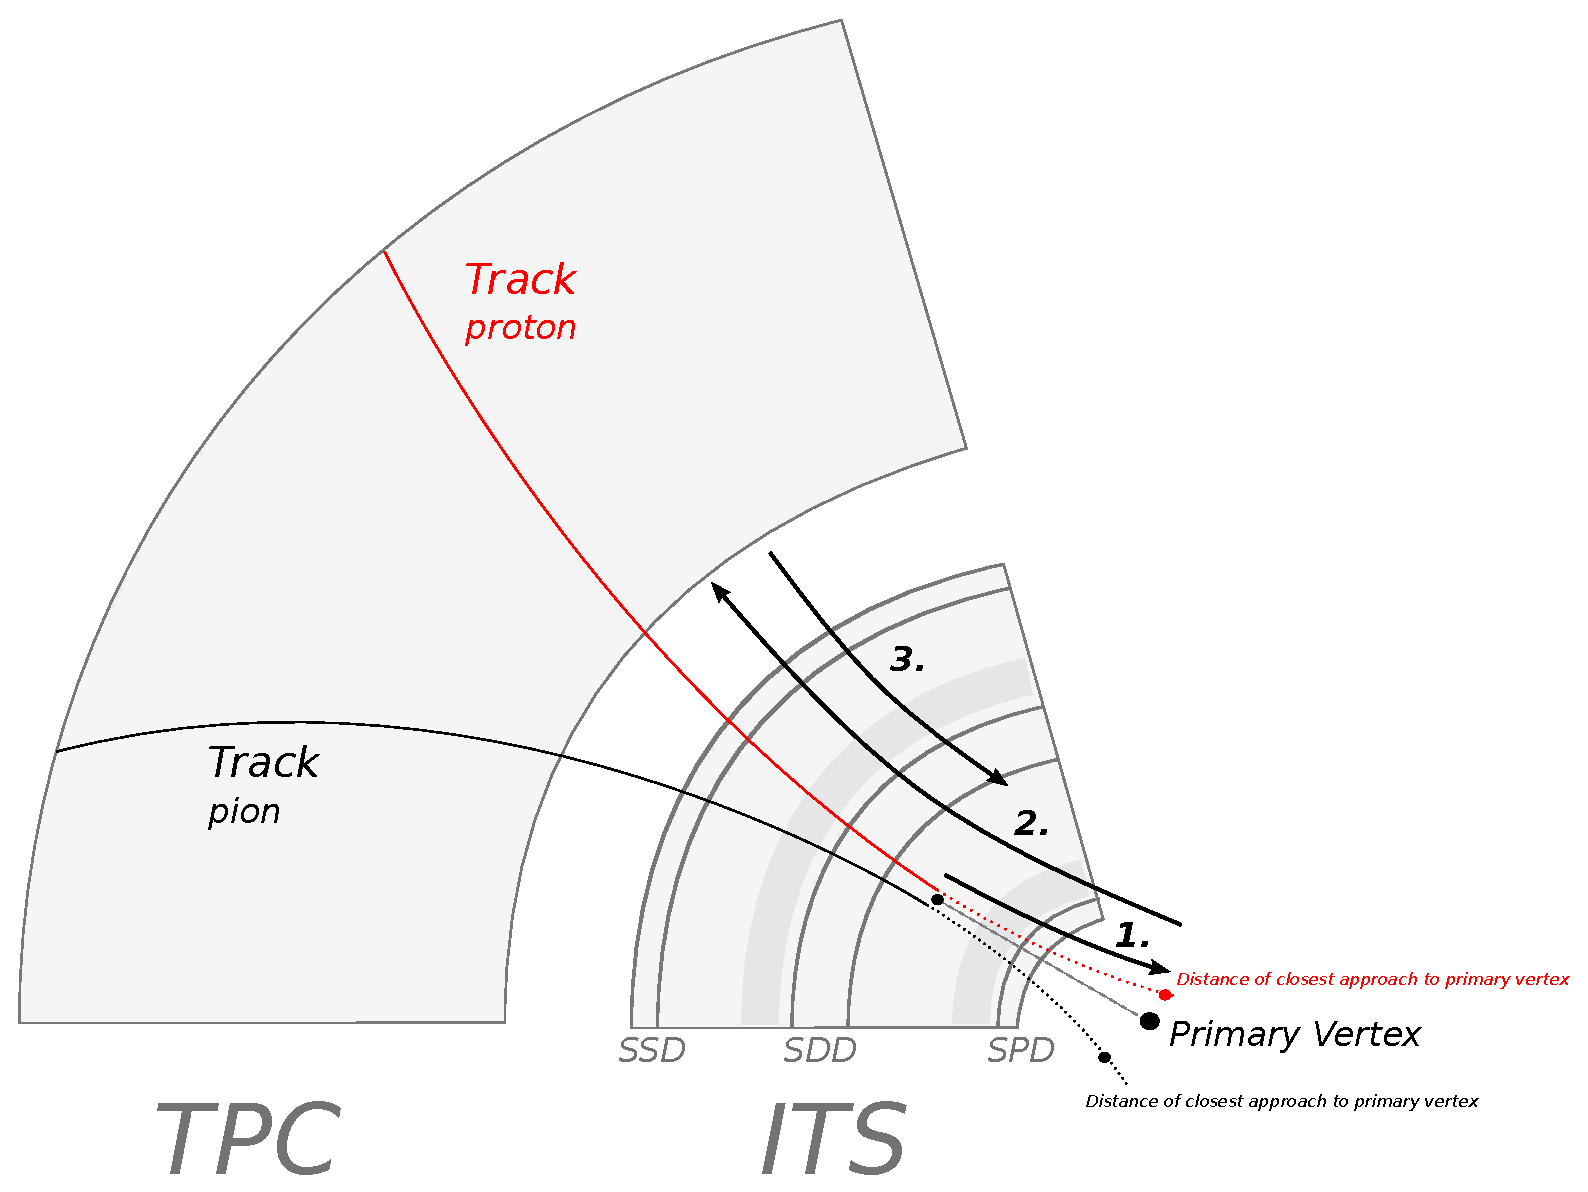
\includegraphics[width=1\textwidth]{Figs/Chapter5/Schema-RetroCorrections.eps}
	\caption{Pictural representation of the fix on the energy loss corrections applied on the proton daughter of a \rmLambdaPM. The general idea breaks off in two stages: removing the previous \dEdx-corrections below the TPC inner wall (1. and 2.), and re-applying them appropriately (3.). The first stage starts with the propagation of the track parameters, initially at the decay position, to its DCA to the primary vertex without accounting for energy loss (1.). Then, the track is propagated to the TPC inner wall (2.) as performed during the final stage of the tracking (\Sec\ref{subsubsec:TrackReco}). In the second stage, the energy loss corrections are re-applied with the correct mass hypothesis -- here, the proton mass -- and stopping at the secondary vertex position (3.). Modified version of the figure from \cite{maireTrackReconstructionPrinciple2011}.}
	\label{fig:SchemeRetroCorrection}
\end{figure}

The procedure starts off with the track parameters at the V0/cascade decay point. They are extrapolated to its point of closest approach to the primary vertex, without accounting for energy losses (\fig\ref{fig:SchemeRetroCorrection}, 1.). This basically means undoing the track propagation in \Sec\ref{subsubsec:V0Formation} and recover the track parameters as they were before the V0/cascade reconstruction. From this point, the track is propagated to its position at the TPC inner wall, in the exactly same condition as in the final stage of the tracking (\Sec\ref{subsubsec:TrackReco}): same mass hypothesis, same consideration on the detector material. This means that, at each step, the track looses the identical amount of energy which was previously added. At the TPC inner wall, the aforementioned energy loss corrections \textit{in the ITS} have been fully\break removed (\fig\ref{fig:SchemeRetroCorrection}, 2.). As most of the material budget comes from the ITS, the wrong energy loss corrections in the TPC can be ignored in first approximation. This last point was later verified with a propagation up to the TPC outer wall; no~significant change could have been observed.  

The second stage takes over with the re-application of the energy loss corrections. From the TPC inner wall, the track parameters are propagated to the secondary vertex position with the appropriate mass hypothesis and the adequate material, in order to correct the right amount of energy losses this time (\fig\ref{fig:SchemeRetroCorrection}, 3.).\\

\begin{figure}[p]
%\centering
\hspace*{-2.cm}
\subfigure[]{
	\includegraphics[width=0.6\textwidth]{Figs/Chapter5/MassVsRadius\_XiWithRetroCorr\_MC.eps}
	\label{fig:MassVsRadiusXiMCRetroCorr}
} 
\subfigure[]{
	\includegraphics[width=0.6\textwidth]{Figs/Chapter5/MassVsRadius\_XiWithRetroCorr.eps}
	\label{fig:MassVsRadiusXiRetroCorr}
} 
\hspace*{-2.cm}
\subfigure[]{
	\includegraphics[width=0.6\textwidth]{Figs/Chapter5/MassVsRadius\_OmegaWithRetroCorr\_MC.eps}
	\label{fig:MassVsRadiusOmegaMCRetroCorr}
} 
\subfigure[]{
	\includegraphics[width=0.6\textwidth]{Figs/Chapter5/MassVsRadius\_OmegaWithRetroCorr.eps}
	\label{fig:MassVsRadiusOmegaRetroCorr}
} 
\caption{Measured mass of the \rmXi (top) and \rmOmega baryons (bottom), in MC (left) and in the data (right), as a function of the \textbf{cascade decay radius} with the retro-corrections on (red) and off (blue). The regions close to ITS layers have been removed, as explained in \Sec\ref{subsubsec:DecayRadiusDependence}. The solid and dashed lines represent a fit with a constant function. Note that, for the purpose of the comparison, the MC is \textit{not} re-weighted (\Sec\ref{subsubsec:CorrectionOnTheExtractedMass}). In both cases, the results have been obtained through a fit with a triple Gaussian function for the invariant mass peak and, only in the data, an exponential function for the background.}
	\label{fig:MassVsRadiusAfterRetrocorrection}
\end{figure}

\Fig\ref{fig:MassVsRadiusAfterRetrocorrection} shows the application of this procedure in the data and MC. The retro-corrections significantly reduces the mass offset with the decay radius. Most importantly, in MC, the trend with the radius has disappeared and now follows a flat distribution. To quantify it, the measurements have been fitted with a constant function; the latter agrees very well the injected mass of \rmXi and displays a $\chi^{2}$ probability of at least 26\%. This validates that the energy losses are now properly taken into account. In the data, a slight trend with radius can still be observed. This will flatten in the next sections in such way that, in the end, the residual dependence on the radius can be considered as negligible. 


\subsubsection{Dependence on momentum}
\label{subsubsec:MassDependenceOnPt}

Although the invariant mass expression in \eq\ref{eq:CascInvMass} involves only the momentum vector of the decay daughters, it can be re-written to show the \textit{explicit} dependence on the total momentum in \eq\ref{eq:InvMassPtotDependenceCasc},
\begin{align}
M_{\rm candidate}^2( \textrm{casc.}) &= \Big(\sqrt{ \textbf{p}_{\rm V0}^2 + m_{\rmLambda}^2} + \sqrt{ \textbf{p}_{\rm bach.}^2 + m_{\rm bach.}^2}\Big)^2 - ( \textbf{p}_{\rm V0} + \textbf{p}_{\rm bach.})^2 \\
&= \Big(\sqrt{ p_{\rm V0}^2 + m_{\rmLambda}^2} + \sqrt{ p_{\rm bach.}^2 + m_{\rm bach.}^2}\Big)^2 - \left( p_{\rm V0}^{2} + p_{\rm bach.}^{2} + 2 \cdot p_{\rm V0} \cdot p_{\rm bach.} \cos \theta \right),
\label{eq:InvMassPtotDependenceCasc}
\end{align}
and in particular, the \textit{explicit} dependence on the transverse and longitudinal momenta in \eq\ref{eq:InvMassPtPzDependenceCasc},
\begin{equation}
\begin{split}
M_{\rm candidate}^2( \textrm{casc.}) &= \Big(\sqrt{ p_{\rm T, V0}^2 + p_{\rm z, V0}^2 + m_{\rmLambda}^2} + \sqrt{ p_{\rm T, bach.}^2 + p_{\rm z, bach.}^2 + m_{\rm bach.}^2}\Big)^2 \\
&\quad - \big( p_{\rm T, V0}^{2} + p_{\rm T, bach.}^{2} + 2 \cdot p_{\rm T, V0} \cdot p_{\rm T, bach.} \cos \theta_{xy}\\
&\quad + p_{\rm z, V0}^{2} + p_{\rm z, bach.}^{2} + 2 \cdot p_{\rm z, V0} \cdot p_{\rm z, bach.} \cos \theta_{z} \big),
\end{split}
\label{eq:InvMassPtPzDependenceCasc}
\end{equation}
where $\theta$, $\theta_{xy}$ and $\theta_z$ are the opening angles in 3D, in the transverse plane and in the longitudinal direction, defined in the laboratory frame.

It becomes clear that the invariant mass depends on both momenta and opening angles. Any systematic effect on those variables would immediately bias the invariant mass distributions, and thus the measured mass.

\begin{figure}[!p]
%\centering
\hspace*{-2.cm}
\subfigure[]{
	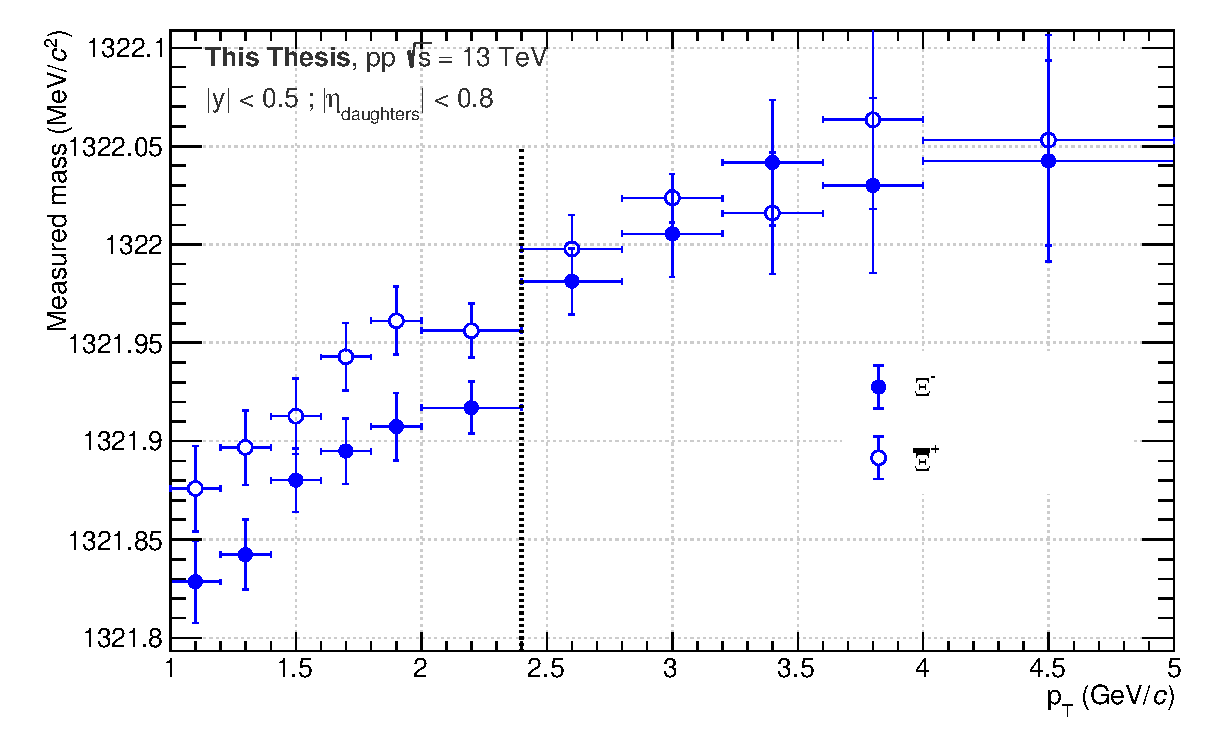
\includegraphics[width=0.6\textwidth]{Figs/Chapter5/InvMassXiVsPt.eps}
	\label{fig:MassVsPtXi}
} 
\subfigure[]{
	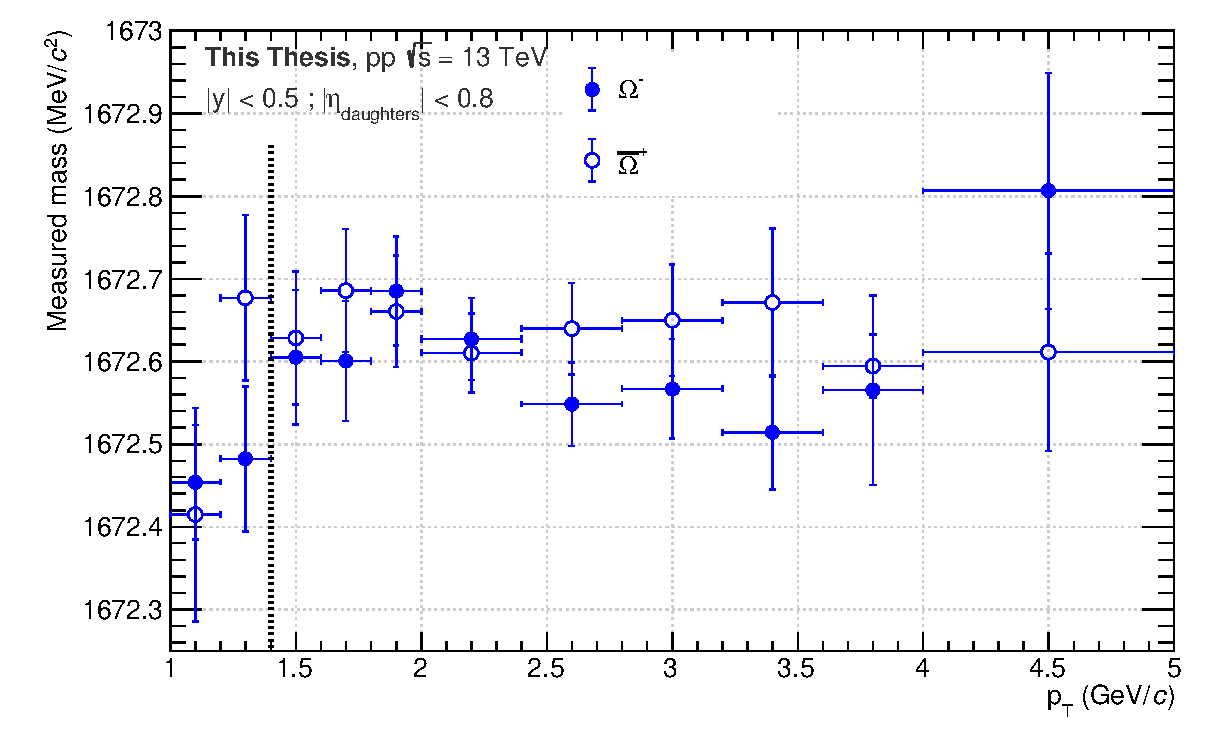
\includegraphics[width=0.6\textwidth]{Figs/Chapter5/InvMassOmegaVsPt.eps}
	\label{fig:MassVsPtOmega}
} 
\caption{Measured mass of the \rmXi (top) and \rmOmega baryons (bottom) as a function of the \textbf{transverse momentum}. The dashed line represents the transverse momentum threshold, where the mass values can be considered as stable. In both cases, the results have been obtained through a fit with a triple Gaussian function for the invariant mass peak and, only in the data, an exponential function for the background.}
	\label{fig:MassVsPt}
\end{figure}

\begin{figure}[!p]
%\centering
\hspace*{-2.cm}
\subfigure[]{
	\includegraphics[width=0.6\textwidth]{Figs/Chapter5/MassXi\_pz\_Aside\_MC.eps}
	\label{fig:MassVsPzXiMC}
} 
\subfigure[]{
	\includegraphics[width=0.6\textwidth]{Figs/Chapter5/MassXi\_pz\_Aside.eps}
	\label{fig:MassVsPzXi}
} 
\caption{Measured mass of the \rmXi hyperons as a function of the \textbf{longitudinal momentum}. The solid and dashed lines represent a fit with a constant function. In both cases, the results have been obtained through a fit with a triple Gaussian function for the invariant mass peak and, only in the data, an exponential function for the background.}
	\label{fig:MassXiVsPz}
\end{figure}


\Fig\ref{fig:MassVsPt} shows the measurd mass of the \rmXi and \rmOmega baryons as a function of the transverse momentum. At low \pT, the measured masses change rapidly with the transverse momentum, due to multiple scattering and (asymmetric) energy loss fluctuations. The latter becomes less dominant at intermediate \pT, and so this scaling reduces such that a flat dependence is reached at intermediate or high transverse momentum. 

In order to ensure stable measurements with \pT, the analysis should be performed in this plateau region. Although the \rmKzeroS and \rmLambda follows the same V0 decay topology, their decay kinematics are different. This also holds for the \rmXi and \rmOmega baryons. Thereby, the position of this stability region has to be identified separately for each particle. For instance, the data points above $\pT > 2$ \gmom for the \rmLambda in \fig\ref{fig:MassVsPtXi} and $\pT > 2.4$ \gmom for the \rmXi in \fig\ref{fig:MassVsPtOmega} show little variations with the transverse momentum, and are all contained with a $1\sigma$ interval around the final measurement, after accounting for all the other sources of systematic effects. Therefore, in this region, the measurement can be considered as under control.\\

Along the same line, the influence of the longitudinal momentum on the measured mass has been checked. It is presented in \fig\ref{fig:MassXiVsPz}. Both in the data and in MC, the dependence remains relatively small, such that it can be considered as negligible in the considered (pseudo-)rapidity interval.


\subsubsection{Dependence on the opening angles}
\label{subsubsec:OpAngleDependence}

As discussed above, the invariant mass depends on the opening angle between the decay products. Due to the multiple scattering, the latter may increase or decrease, thus biasing the estimation of the decay vertex position (as observed in \fig\ref{fig:MassVsRadius}) and the measured mass. 

Therefore, different opening angles in the laboratory frame are being considered:

\begin{itemize}
\item[$\bullet$] \textbf{the opening angle in 3 dimensions}, also called \textit{3D opening angle}. \\
There are two ways to compute this quantity, depending on whether the value must be signed or unsigned. Here, it has been decided that value of the opening angle would be unsigned. It can be calculated from the momentum vectors of the positive and negative decay daughters:
\begin{align}
&{\bf p_{\rm pos.}} \cdot {\bf p_{\rm neg.}} = p_{\rm pos.} p_{\rm neg.} \cos\left(\theta\right) \\
\Rightarrow \qquad &\theta = \arccos \frac{ \left( {\bf p_{\rm pos.}} \cdot {\bf p_{\rm neg.}} \right)}{ p_{\rm pos.} \ p_{\rm neg.}}
\label{eq:OpeningAngle3D}
\end{align}

\item[$\bullet$] \textbf{the transverse opening angle}.\\
Here, the sign of the opening angle in the transverse plane might be important, as it relates to two vertex configurations, said \say{cowboy} and \say{sailor}~\cite{chinellatoTwotrackDCACalculation2018}. When reconstructing a V0, a search for the minimum distance of closest approach between two oppositely charged tracks is performed as illustrated in \fig\ref{fig:TwoTrackDCACalculationIdealCase}. However, this approach reaches its limit in case there are two minima, as in \fig\ref{fig:TwoTrackDCACalculationCowboySailor}. In such case, there is an ambiguity on the position of the DCA between the two tracks which, depending on the point taken as  V0 decay vertex, may lead to a bias in the momentum and thus in the reconstructed mass\footnote{There actually exists a procedure -- used in this analysis -- implemented in the V0 and cascade vertexing algorithm to lift this ambiguity. It consists in finding \textit{analytically} the possible positions of the decay vertex in the transverse plane, using them as a starting point to compute the distance of closest approach in 3-dimensions for each vertex candidate and selecting the one providing the minimum DCA \cite{chinellatoTwotrackDCACalculation2018}.}. The same argument could be made for cascade decays.

\begin{figure}[h]
\subfigure[]{
	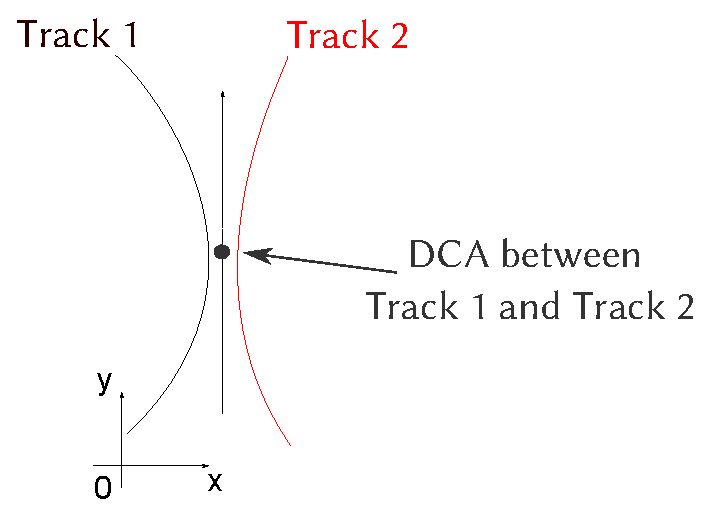
\includegraphics[width=0.5\textwidth]{Figs/Chapter5/IdealCase.eps}
	\label{fig:TwoTrackDCACalculationIdealCase}
}
\subfigure[]{
	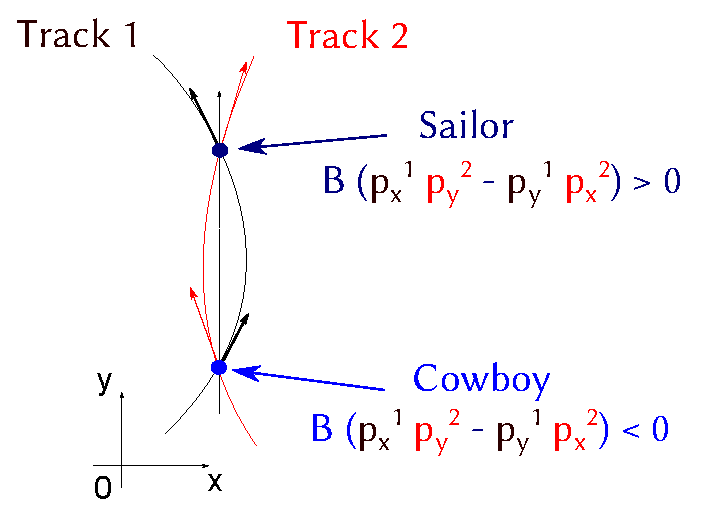
\includegraphics[width=0.5\textwidth]{Figs/Chapter5/CowboySailor.eps}
	\label{fig:TwoTrackDCACalculationCowboySailor}
}
\caption{Sketch of the distance of closest approach (DCA) between two tracks in (a) the most expected case, and in (b) the cowboy and sailor configurations. The reconstructed vertex is said to be in sailor configuration if $ B \left( p_{x, \text{pos.}} \ p_{y, \text{neg.}} - p_{x, \text{neg.}} \ p_{y, \text{pos.}} \right)~>~0$, with $B$ the magnetic field. Conversely, it is in cowboy configuration if $ B \left( p_{x, \text{pos.}} \ p_{y, \text{neg.}} - p_{x, \text{neg.}} \ p_{y, \text{pos.}} \right) < 0$.}
	\label{fig:TwoTrackDCACalculation}
\end{figure}

To obtain a signed angle, one takes the cross product between the momentum vectors of the decay daughters:
\begin{align}
&{\bf p_{\rm pos.}} \times {\bf p_{\rm neg.}} = p_{\rm pos.} p_{\rm neg.} \sin\left(\theta_{xy}\right) \ {\bf n} \\
\Rightarrow \qquad &\theta_{xy} = \arcsin \frac{ \left( {\bf p_{\rm pos.}} \times {\bf p_{\rm neg.}} \right) \cdot {\bf n}}{ p_{\rm pos.} \ p_{\rm neg.}}
\label{eq:OpeningAngle2D}
\end{align}

\item[$\bullet$] \textbf{the longitudinal opening angle}.\\
Finally, the opening angle in the longitudinal direction, $\theta_z$ can be deduced directly from the difference of longitudinal angle between the two decay daughters :
\begin{equation}
\theta_{z} = \theta_{z, \textrm{pos.}} - \theta_{z, \textrm{neg.}}
\label{eq:OpeningAngleZ}
\end{equation}
\end{itemize}

\begin{figure}[!p]
%\centering
\hspace*{-2.cm}
\subfigure[]{
	\includegraphics[width=0.6\textwidth]{Figs/Chapter5/MassVsOpeningAngle\_MC.eps}
	\label{fig:MassVsOpeningAngle3DLambdaMC}
} 
\subfigure[]{
	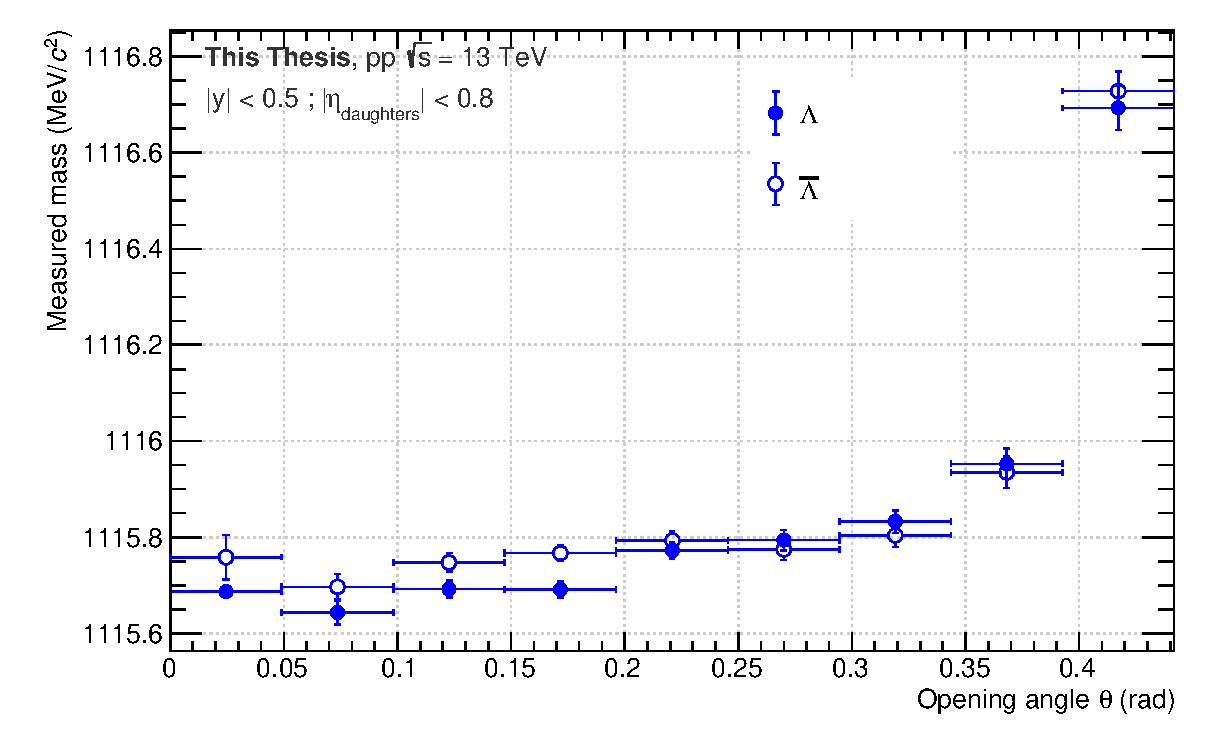
\includegraphics[width=0.6\textwidth]{Figs/Chapter5/MassVsOpeningAngle.eps}
	\label{fig:MassVsOpeningAngle3DLambda}
} 
\hspace*{-2.cm}
\subfigure[]{
	\includegraphics[width=0.6\textwidth]{Figs/Chapter5/MassVsOpeningAngleXY\_MC.eps}
	\label{fig:MassVsOpeningAngle2DLambdaMC}
} 
\subfigure[]{
	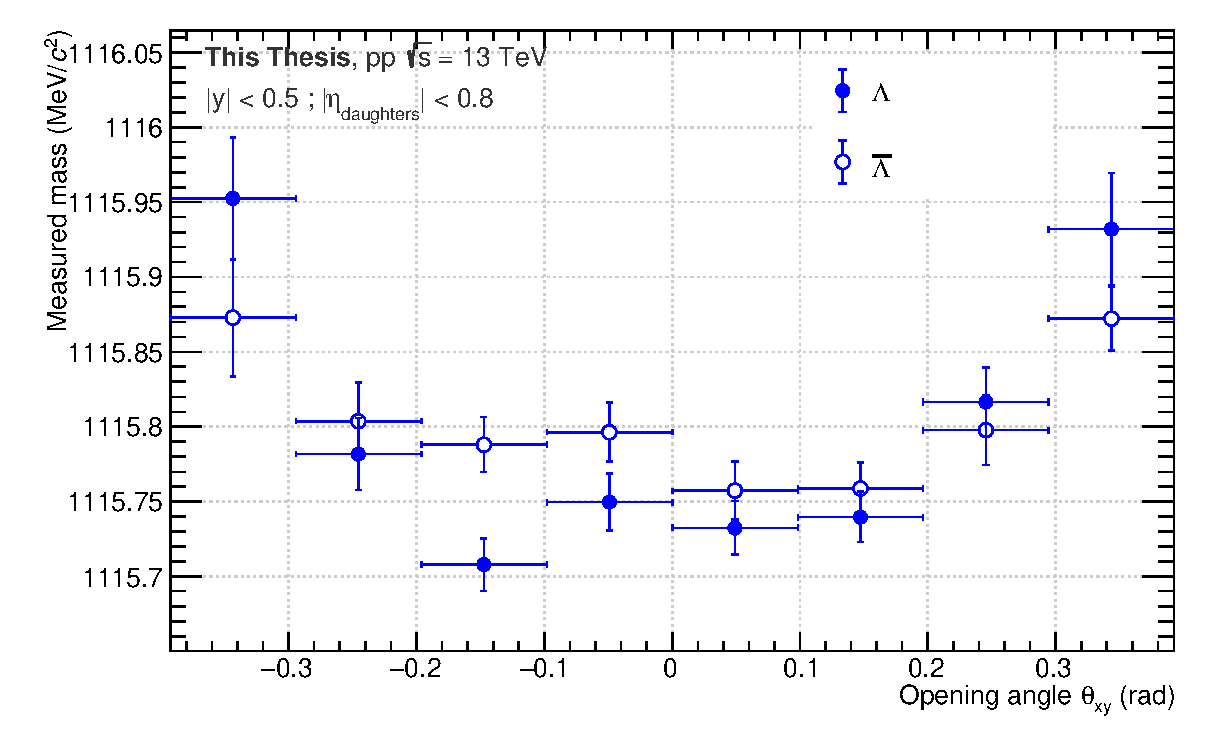
\includegraphics[width=0.6\textwidth]{Figs/Chapter5/MassVsOpeningAngleXY.eps}
	\label{fig:MassVsOpeningAngle2DLambda}
} 
\hspace*{-2.cm}
\subfigure[]{
	\includegraphics[width=0.6\textwidth]{Figs/Chapter5/MassVsOpeningAngleZ\_MC.eps}
	\label{fig:MassVsOpeningAngleZLambdaMC}
} 
\subfigure[]{
	\includegraphics[width=0.6\textwidth]{Figs/Chapter5/MassVsOpeningAngleZ.eps}
	\label{fig:MassVsOpeningAngleZLambda}
} 
\caption{Measured mass of the \rmLambda as a function of the \textbf{opening angle} in three dimensions, in the transverse plane as well as in the longitudinal direction, in MC on the left and in the data on the right. Note that, for the purpose of the comparison, the MC is \textit{not} re-weighted (\Sec\ref{subsubsec:CorrectionOnTheExtractedMass}). In both cases, the results have been obtained through a fit with a triple Gaussian function for the invariant mass peak and, only in the data, an exponential function for the background.}
	\label{fig:MassVsOpeningAngleLambda}
\end{figure}

\begin{figure}[h]
%\centering
\hspace*{-2.cm}
\subfigure[]{
	\includegraphics[width=0.6\textwidth]{Figs/Chapter5/MassVsOpeningAngleXY\_MC.eps}
	\label{fig:MassVsOpeningAngleXY}
} 
\subfigure[]{
	\includegraphics[width=0.6\textwidth]{Figs/Chapter5/OpAngle2DVsAvgDecayRadiusResol\_Lambda.eps}
	\label{fig:DecayVtxResolVsOpeningAngle}
} 
\caption{On the left: the measured mass of \rmLambda hyperons as a function of the \textbf{transverse opening angle} in MC data. On the right: the average resolution on the decay radius as a function of the very same opening angle.}
	\label{fig:MassVsOpeningAngle}
\end{figure}

\Fig\ref{fig:MassVsOpeningAngleLambda} shows the distributions of the extracted mass of \rmLambda and \rmAlambda as a function of the different opening angles. All display the same trend, namely the measured mass is relatively high for large opening angle values and decreases with the opening angles until reaching a flat region close to the small opening angles. Furthermore, this pattern being well reproduced in the simulations, its origin can be investigated by making use of the MC truth. 

In \fig\ref{fig:MassVsOpeningAngle}, the average resolution on the radial position of the decay vertex as a function of the transverse opening angle in MC simulations is shown. At large opening angle, the resolution on the decay vertex is quite poor: it tends to be located at a larger radius. It results in an over-estimation of the momentum of each decay daughters, and so in an increase of the reconstructed mass. As the opening angle becomes narrower, the resolution on the decay vertex improves and the momentum bias decreases. \Fig\ref{fig:MassVsOpeningAngle} only serves as an example; the same trend is observed for the opening angles in three dimensions and along the $z$-axis. To tackle that issue, the strategy followed by the present analysis consists to reject candidates with too large opening angles, for \rmKzeroS, \rmLambda, \rmAlambda, \rmXiPM and \rmOmegaPM. In this way, one also manages to obtain flat distribution of the measured mass as a function of these variables.\\

\subsubsection{Dependence on the azimuthal angles}
\label{subsubsec:DependenceAzimuthalAngle}

ALICE being a cylindrical detector, any (decay) point can be identified based on its distance from the origin $r$ and its azimuthal angle $\varphi$ in the transverse plane, as well as its longitudinal position $z$. \Sec\ref{subsubsec:DecayRadiusDependence} investigated how the reconstructed mass varies as a function of the decay radius; along the same line, the dependence with the transverse direction of the decay can also be studied.

Two definitions exist concerning the angle in the transverse plane; there are the \textit{position} and the \textit{momentum} azimuthal angles. The former refers to the spatial coordinate around the $z$-axis, the latter corresponds to the same coordinate but in momentum space. In other words, one can be calculated from the radial decay position, the other, using the transverse momenta. For a neutral particle, such as the \rmKzeroS and \rmLambda, these two angles should coincide\footnote{Assuming that the V0 originates from the primary vertex.}, whereas it should not for charged particles, including the \rmXi or \rmOmega. Due to their relatively short flight distance, the difference between these two angles for multi-strange baryons turns out to be negligible. Consequently, the term \textit{azimuthal angle} will be used to designate the momentum one, unless indicated otherwise.

The ALICE volume has been divided into eighteen even azimuthal sectors: nine for the top barrel, and nine for the bottom barrel. This study employs such segmentation as it coincides with the TPC sectors (\fig\ref{fig:TPCDetector}), and thus may help to relate a possible pattern to problematic sectors.\\

\Figs\ref{fig:MassVsACPhi}, \ref{fig:MassVsPhiVsB}, \ref{fig:MassVsPhiAVsC} show the dependence on the momentum azimuthal angle for \rmKzeroS, \rmLambda, \rmXi in MC on the left hand-side, and in the data on the right hand-side. The measured masses vary strongly from one angular sector to the next, in the data \figs\ref{fig:MassVsPhiACK0s}, \ref{fig:MassVsPhiACLambda}, \ref{fig:MassVsPhiACXi}. A pattern emerges for all the considered particles: on the edges, the measurement points stay relatively at the same level, and change drastically as they approach $\varphi \simeq \pi$. At such location, the \rmLambda and \rmXi masses gain up to 200 \kmass, and up to 1.2 \mmass for the \rmKzeroS. In constrast, the masses extracted in MC simulations exhibit a relatively flat dependence with the azimuthal angle, compatible with a constant function with a $\chi^{2}$ probability varying between 1\% and 86\%. The trend observed in real data is not reproduced in the simulations, suggesting that one or several elements of the experiment are not accounted for in the MC productions.

\begin{figure}[!p]
%\centering
\hspace*{-1.5cm}
\subfigure[]{
	\includegraphics[width=0.6\textwidth]{Figs/Chapter5/MassK0s\_MomPhi\_ACsides\_MC.eps}
	\label{fig:MassVsPhiACMCK0s}
} 
\subfigure[]{
	\includegraphics[width=0.6\textwidth]{Figs/Chapter5/MassK0s\_MomPhi\_ACsides.eps}
	\label{fig:MassVsPhiACK0s}
} 
\hspace*{-1.5cm}
\subfigure[]{
	\includegraphics[width=0.6\textwidth]{Figs/Chapter5/MassLambda\_MomPhi\_ACsides\_MC.eps}
	\label{fig:MassVsPhiACMCLambda}
} 
\subfigure[]{
	\includegraphics[width=0.6\textwidth]{Figs/Chapter5/MassLambda\_MomPhi\_ACsides.eps}
	\label{fig:MassVsPhiACLambda}
} 
\hspace*{-1.5cm}
\subfigure[]{
	\includegraphics[width=0.6\textwidth]{Figs/Chapter5/MassXi\_MomPhi\_ACsides\_MC.eps}
	\label{fig:MassVsPhiACMCXi}
} 
\subfigure[]{
	\includegraphics[width=0.6\textwidth]{Figs/Chapter5/MassXi\_MomPhi\_ACsides.eps}
	\label{fig:MassVsPhiACXi}
}  
\caption{Measured mass in pp collisions at \sqrtS = 13 \tev as a function of the momentum \textbf{azimuthal angle}. Results in simulated data are presented on the left-hand side, while those in real data can be found on the right-hand side. To each row corresponds a given particle: \rmKzeroS (a) and (b), \rmLambda (c) and (d), \rmXi in (e) and (f). The uncertainties comprise only the statistical ones.}
	\label{fig:MassVsACPhi}
\end{figure}

\begin{figure}[!p]
%\centering
\hspace*{-1.5cm}
\subfigure[]{
	\includegraphics[width=0.6\textwidth]{Figs/Chapter5/MassLambda\_MomPhi\_ACsides\_NegB.eps}
	\label{fig:MassVsPhiNegBLambda}
} 
\subfigure[]{
	\includegraphics[width=0.6\textwidth]{Figs/Chapter5/MassLambda\_MomPhi\_ACsides\_PosB.eps}
	\label{fig:MassVsPhiPosBLambda}
} 
\hspace*{-1.5cm}
\subfigure[]{
	\includegraphics[width=0.6\textwidth]{Figs/Chapter5/MassXi\_MomPhi\_ACsides\_NegB.eps}
	\label{fig:MassVsPhiNegXi}
} 
\subfigure[]{
	\includegraphics[width=0.6\textwidth]{Figs/Chapter5/MassXi\_MomPhi\_ACsides\_PosB.eps}
	\label{fig:MassVsPhiPosBXi}
}   
\caption{Measured mass in pp collisions at \sqrtS = 13 \tev as a function of the momentum \textbf{azimuthal angle} in two opposite magnetic field polarities: $\mathbf{B = -0.5}$ \textbf{T} on the left, and $\mathbf{B=+0.5}$ \textbf{T} on the right. To each row corresponds a given particle: \rmLambda (a) and (b), \rmXi in (c) and (d). The uncertainties comprise only the statistical ones.}
	\label{fig:MassVsPhiVsB}
\end{figure}

\begin{figure}[!p]
%\centering
\hspace*{-1.5cm}
\subfigure[]{
	\includegraphics[width=0.6\textwidth]{Figs/Chapter5/MassK0s\_MomPhi\_Csides.eps}
	\label{fig:MassVsPhiCsideK0s}
} 
\subfigure[]{
	\includegraphics[width=0.6\textwidth]{Figs/Chapter5/MassK0s\_MomPhi\_Asides.eps}
	\label{fig:MassVsPhiAsideK0s}
} 
\hspace*{-1.5cm}
\subfigure[]{
	\includegraphics[width=0.6\textwidth]{Figs/Chapter5/MassLambda\_MomPhi\_Csides.eps}
	\label{fig:MassVsPhiCsideLambda}
} 
\subfigure[]{
	\includegraphics[width=0.6\textwidth]{Figs/Chapter5/MassLambda\_MomPhi\_Asides.eps}
	\label{fig:MassVsPhiAsideLambda}
} 
\hspace*{-1.5cm}
\subfigure[]{
	\includegraphics[width=0.6\textwidth]{Figs/Chapter5/MassXi\_MomPhi\_Cside.eps}
	\label{fig:MassVsPhiCsideXi}
} 
\subfigure[]{
	\includegraphics[width=0.6\textwidth]{Figs/Chapter5/MassXi\_MomPhi\_Aside.eps}
	\label{fig:MassVsPhiAsideXi}
}  
\caption{Measured mass in pp collisions at \sqrtS = 13 \tev as a function of the momentum \textbf{azimuthal angle in C-side} (left) and \textbf{A-side} (right) of the ALICE detector. To each row corresponds a given particle: \rmKzeroS (a) and (b), \rmLambda (c) and (d), \rmXi in (e) and (f). The uncertainties comprise only the statistical ones. Beware the fact that the ordinate ranges differ here between the C-side and A-side panels.}
	\label{fig:MassVsPhiAVsC}
\end{figure}

Different possible origins for this \say{odd} behaviour have been investigated:
\begin{enumerate}
\item One possible explanation involves the material distribution within the detector. \Sec\ref{subsubsec:ImperfectEnergyLossCorrections} provides a short explanation on how the material budget is evaluated in ALICE. This section also provides a systematic uncertainty on our mass measurement, which proves to be too small to account for the large mass variations in \figs\ref{fig:MassVsACPhi}. Nevertheless, it is \textit{a priori} possible that some material have not been taken into account in the detector geometry. In particular, an underestimated amount of material budget in the region $\varphi \simeq \pi$ could explain the trend. In such a case, this structure is expected to change with the radial position of the decay vertex, as a V0/cascade decaying beyond the region with additional or underestimated material budget should not be affected by it. However, it turns out that the decay radius of the V0 and/or cascade shows no influence on the azimuthal trend.
\item Another attempt at an explanation concerns the alignement of the ALICE detector, and in particular the ITS. As in the first point with the material distribution, the discrepancy between the data and the MC may be related to residual misalignement. The strategy followed to test this hypothesis is to repeat the whole analysis but using TPC-standalone tracks instead of global tracks. The TPC is expected to be better calibrated and internally aligned than the ITS, a change in the azimuthal dependence on the measured mass would point towards an issue related to the alignment. After repeating the analysis with TPC standalone tracks, the shape of the structure changes slightly but a peak still emerges around an azimuthal angle of $\pi$.
\item In order to shed light on that issue, the data sample has been divided into two sub-samples according to their magnetic field polarity. Maybe this trend originates only from periods with a specific magnetic field. \Fig\ref{fig:MassVsPhiVsB} shows the distribution of the measured mass as a function of $\varphi$. The same trend is observed in both sub-samples though, interestingly, the peaks in the vicinity of $\varphi = \pi$  for the particle and the anti-particle (\rmLambda and \rmAlambda, and \rmXiM and \rmAxiP) are swapped under an inversion of magnetic field polarity. This tells us that this structure is somehow related to the magnetic field.
\item Similarly, the V0 and cascade candidates have been separated based on the longitudinal position of decay and, in particular, whether they locate on the positive or negative $z$-side\footnote{Here, this is a constraint on the whole decay. In other words, this means that the decay must happen on either the positive or negative $z$-side, and all the decay products have to remain on the very same side. Note also that the region of the central membrane of the TPC ($z = 0$) is excluded.}. As mentioned in the header of \Sec\ref{subsec:ALICEDetector}, these are also referred as A-side and C-side respectively. The comparison of the azimuthal dependence on the measured mass in these two sides is displayed on \fig\ref{fig:MassVsPhiAVsC}. On the left hand-side panels \figs\ref{fig:MassVsPhiCsideK0s},\ref{fig:MassVsPhiCsideLambda},\ref{fig:MassVsPhiCsideXi} corresponding to the C-side, the dependence is still present. However, it reduces significantly on the A-side (\figs\ref{fig:MassVsPhiAsideK0s},\ref{fig:MassVsPhiAsideLambda},\ref{fig:MassVsPhiAsideXi}), such that it almost follows a flat distribution. Although the \rmKzeroS masses still fluctuate with the azimuthal angle, the magnitude of the variations is smaller on the A-side. Therefore, the origin of such dependence has to be found on the C-side. Amongst its singularities, the most noteworthy are certainly the presence of the muon arm absorber and the dipole magnet. In the past, the former was observed to be the source of many secondary particles, originating from the interaction with absorber material. This can, in turn, distort the background distribution in the invariant mass spectra, leading possibly to a difference in terms of extracted mass. This is rather unlikely in the present conditions of the analysis; the tight selection on the cosine of the pointing angle allows to reach purities above 95\% for the V0s and 90\% for the cascades. At such level of background, it would be surprising to find it at the origin of this dependence\footnote{As a matter of fact, the level of background as a function of the azimuthal angle has been checked. No correlation with the azimuthal dependence on the measured mass has been seen.}. On the other hand, the dipole magnet has an influence on the magnetic field within the L3 magnet. The induced distortions have been assessed in the collaboration and accounted for in the detector calibration. However, there may still be some residual distortions that could affect the particle trajectory and ultimately lead to a variation of the reconstructed mass with the TPC sector. On top of that, the magnetic field is supposed to coincide with the $z$-axis, with the electric field in the TPC cage; if not (due to a distortion induced by the dipole magnet), the so-called $E\times B$ effects can bias the measurement of the particle trajectory, by curling the electrons around their main drift path towards the end plate. This would lead to a systematic displacement of the associated clusters, which later impact the tracking and finally the invariant mass.
\end{enumerate}

In summary, the origin of the azimuthal dependence cannot be claimed for sure. It appears clearly, from \figs\ref{fig:MassVsPhiAVsC}, that the analysis should focus on the A-side of the detector. The residual variations of the measured mass, those that cannot be accounted for by other sources of systematic biases, should be evaluated and encapsulated as a systematic uncertainty. Hence, this systematic effect introduces an uncertainty of 0.256, 0.056, 0.084 and 0.081 \mmass on the mass values of the \rmKzeroS, \rmLambdaPM, \rmOmegaM and \rmAomegaP\footnote{Although not shown here for the sake of brievety, the \rmOmegaPM baryons have also been investigated along their possible azimuthal dependence.} respectively. Notice that only the \rmXi baryons remain  unaffected by the variation with the azimuth; this will be explained later in \Sec\ref{subsec:CorrectionOnTheExtractedMass}. In addition, the effect on the mass difference have been observed to be mild. Therefore, no additionnal systematic uncertainty is attributed to the mass difference values.

\subsubsection{Dependence on the rapidity}
\label{subsubsec:RapidityDependence}

The dependence on the $z$ position has somehow already been investigated in \Sec\ref{subsubsec:DependenceAzimuthalAngle} by scrutinising how the measured mass evolves for decays in the A- or C-side. As a cross-check, one can also study the influence of the Lorentz boost along the $z$-axis, namely the rapidity.

\begin{figure}[h]
%\centering
\hspace*{-1.5cm}
\subfigure[]{
	\includegraphics[width=0.6\textwidth]{Figs/Chapter5/MassLambda\_Rap\_Aside\_MC.eps}
	\label{fig:MassVsRapLambdaMC}
} 
\subfigure[]{
	\includegraphics[width=0.6\textwidth]{Figs/Chapter5/MassLambda\_Rap\_Aside.eps}
	\label{fig:MassVsRapLambda}
}
\caption{Measured mass in pp collisions at \sqrtS = 13 \tev as a function of the \textbf{rapidity} of the \rmLambda in MC on the left, and in data on the right. The solid and dashed lines on the left figure represent fits with a constant for the particle and the anti-particle respectively, with a $\chi^{2}$ probability of 38\% and 48\%. The uncertainties comprise only the statistical ones.}
	\label{fig:MassVsRap}
\end{figure}

\Fig\ref{fig:MassVsRap} shows the rapidity dependence on the extracted mass of the \rmLambda hyperon. Following the above discussion (\Sec\ref{subsubsec:DependenceAzimuthalAngle}), the mass is measured on the positive $z$ side of the detector. For that reason, there is no negative rapidity value. The results remain relatively stable over the whole rapidity range; in MC, the data points agree with a flat distribution at 38\% $\chi^{2}$ probability level for the \rmLambda and 48\% for the \rmAlambda. Concerning the data, all the fluctuations can be accounted by other systematic uncertainties. After investigations, we have been led to similar conclusions for \rmKzeroS, \rmXiPM and \rmOmegaPM.


\subsubsection{Dependence on the event multiplicity}
\label{subsubsec:EventMultDependence}

Along the same line as \Sec\ref{subsubsec:DataTakingDependence}, one may wonder whether the results change or not with the event activity, typically quantified by the charged particle multiplicity in the event. The latter is determined using the VZERO detectors as multiplicity estimator, as described in \Sec\ref{subsubsec:VZERO}. The total charge deposited in each VZERO arrays provides a measurement of the charge particle multiplicity, through the calculation of the summed signal amplitude denoted as VZERO-M\footnote{In fact, the VZERO multiplicity estimator corresponds rather to the\break VZERO-M$/\langle \text{VZERO-M}_{\rm MB}\rangle$. This normalisation allows to account for the ageing of the scintillator arrays, that become less transparent over time leading to a deterioration of the detector performances.}. 

\begin{table}[h]
    \centering
    \begin{tabular}{c|ccccc}
    \noalign{\smallskip}\hline \noalign{\smallskip}
    Multiplicity Class & \upperRomannumeral{1} & \upperRomannumeral{2} & \upperRomannumeral{3} & \upperRomannumeral{4} & \upperRomannumeral{5} \\
	\sigmaIdx[]/\sigmaIdx[\INELZero] & 0-0.95\% & 0.95-4.7\% & 4.7-9.5\% & 9.5-14\% & 14-19\% \\	        
	$\langle \dNchdeta \rangle$ & $21.3 \pm 0.6$ & $16.5 \pm 0.5$ & $13.5 \pm 0.4$ & $11.5 \pm 0.3$ & $10.1 \pm 0.3$ \\
	\noalign{\smallskip}\hline \noalign{\smallskip}
	Multiplicity Class & \upperRomannumeral{6} & \upperRomannumeral{7} & \upperRomannumeral{8} & \upperRomannumeral{9} & \upperRomannumeral{10} \\
	\sigmaIdx[]/\sigmaIdx[\INELZero] & 19-28\% & 28-38\% & 38-48\% & 48-68\% & 68-100\% \\
	$\langle \dNchdeta \rangle$ & $8.45 \pm 0.25$ & $6.72 \pm 0.21$ & $5.40 \pm 0.17$ & $3.90 \pm 0.14$ & $2.26 \pm 0.12$ \\
	\noalign{\smallskip}\hline \noalign{\smallskip}
    \end{tabular}
    \caption{Event multiplicity classes, with the corresponding fraction of the total inelastic cross section \INELZero (\sigmaIdx[]/\sigmaIdx[\INELZero]) and average charged particle multiplicity at mid-rapidity in pp at \sqrtS = 7 \tev, $\langle \dNchdeta \rangle$. Table taken from \cite{alicecollaborationMultiplicityDependenceLightflavor2019}.}
    \label{tab:MultiplicityClassesCPT}
\end{table}

The events are divided into ten multiplicity classes, as indicated in \tab\ref{tab:MultiplicityClassesCPT}. \Fig\ref{fig:MassVsMult} shows the dependence of the measured mass of the \rmLambda as a function of the multiplicity. Both in MC and in the data, the measured mass shows little dependence on the event multiplicity, it remains within 50 \kmass range. The same observation has been made for \rmKzeroS, \rmXiPM and \rmOmegaPM, such that the measured mass can reasonably be considered as stable with the event activity.

\begin{figure}[h]
%\centering
\hspace*{-1.5cm}
\subfigure[]{
	\includegraphics[width=0.6\textwidth]{Figs/Chapter5/MassLambda\_Mult\_Aside\_MC.eps}
	\label{fig:MassVsMultLambdaMC}
} 
\subfigure[]{
	\includegraphics[width=0.6\textwidth]{Figs/Chapter5/MassLambda\_Mult\_Aside.eps}
	\label{fig:MassVsMultLambda}
}
\caption{Measured mass in pp collisions at \sqrtS = 13 \tev as a function of the \textbf{event multiplicity percentile} for \rmLambda in MC on the left, and in data on the right. The solid and dashed lines on the left figure represent fits with a constant for the particle and the anti-particle respectively, with a $\chi^{2}$ probability of 8\% and 14\%. The uncertainties comprise only the statistical ones.}
	\label{fig:MassVsMult}
\end{figure}

\subsection{Momentum scale calibration}

The dominant source of systematic uncertainty comes from the momentum scale calibration. This can originate from the uncertainty on the value of the magnetic field (\Sec\ref{subsubsec:ImprecisionMagneticField}) or imperfect energy loss corrections (\Sec\ref{subsubsec:ImperfectEnergyLossCorrections})

\subsubsection{Imprecision on the magnetic field}
\label{subsubsec:ImprecisionMagneticField}

As mentioned in \Sec\ref{subsubsec:DataTakingDependence}, the data sample has been collected with two opposite magnetic field polarities, $B = \pm 0.5$ T. The stability of the measured masses and mass differences have been checked, and the results in different magnetic field configuration have been found to be in good agreement. However, this only guarantees that the calibrations of the ALICE detector between periods of opposite polarities are compatible; nothing can be claimed concerning the precision of such calibrations, and in particular, its influence on the presented results.\\


The measurement of the magnetic field in the L3 magnet has been performed in 2007 and is reported in \cite{shahoyanSummaryL3Magnet2007}. It uses 31 Hall probes, calibrated to a precision of 1 Gauss and distributed over two arms, that could rotate around the beam axis and translate along the very same axis. Based on a set of 480 measurement points, the field was interpolated in order to build the full magnetic field map within the L3 volume. Concerning the precision of the latter, the analysis \cite{shahoyanSummaryL3Magnet2007} concludes the following:
\begin{quote}
\textit{ [...] the difference between the corrected data and the obtained parameterization which gives an estimate of the uncertainty for the latter (on top of the mentioned constant transverse field): within the TPC volume the differences are contained in 2 Gauss range although on the periphery of the scanned region there are points with difference reaching 5-6 Gauss (these points constitute less than 1 \% of all data).} 
\end{quote} 

Since the daughter tracks are required to cross at least 70 readout rows in the TPC, likely distributed over different sectors, the contribution of the points located in the periphery of the scanned region (1 \% of all data) can reasonably be considered as negligible. Therefore, for the whole L3 volume, a 2 Gauss uncertainty on the magnetic field is retained.\\

An uncertainty on the magnetic field translates into a shift of the transverse momentum components of the decay daughters. Transverse momentum is related to magnetic field $B_{0}$ and the track curvature $R$ through the relation ${\pT}_{0} = q B_{0} R$. If the magnetic field $B$ is smaller or greater than its nominal value, $B_{0}$, by 2 Gauss, the transverse momentum would respectively be scaled down or up by a factor $B/B_{0}$:
\begin{equation}
{\pT}_{0} = q B_{0} R \qquad \Rightarrow \qquad \pT = \frac{B}{B_{0}} {\pT}_{0}
\end{equation}

Here is the strategy adopted to evaluate the impact of the magnetic field imprecision: the transverse components of all the decay daughters will be scaled up or down by $B/B_{0}$ -- with $B$ being equal to $B_{0}$ plus or minus 2 Gauss --, the mass will then be extracted as explained in \Sec\ref{subsec:MassExtraction} and the maximum deviation with respect to the measured mass with the nominal value of the magnetic field will be quoted as our uncertainty due to the $B$-field imprecision. The numerical value of the latter can be found in \tab\ref{tab:BFieldPrecision} for \rmKzeroS, \rmLambda, \rmXi and \rmOmega. 

\begin{table}[!h]
    \begin{center}
        \begin{tabular}{l|c|c}       
            \noalign{\smallskip} \hline \noalign{\smallskip}        
            \bf Particle & \multicolumn{2}{c}{\bf Systematic uncertainty on the} \\
            & \bf measured mass & \bf measure mass difference \\
            & \bf (\mmass) & \bf ($\times 10^{-5}$) \\

            \noalign{\smallskip}\hline \noalign{\smallskip}
            \rmKzeroS & 0.080 & /\\
            \noalign{\smallskip}\hline \noalign{\smallskip}
            \rmLambda & 0.013 & negligible\\
            \rmAlambda & 0.013 & negligible\\
            \noalign{\smallskip}\hline \noalign{\smallskip}
            \rmXiM & 0.023 & negligible\\
            \rmAxiP & 0.028 & negligible\\
            \noalign{\smallskip}\hline \noalign{\smallskip}
            \rmOmegaM & 0.026 & negligible\\
            \rmAomegaP & 0.027 & negligible\\
            \noalign{\smallskip}\hline \noalign{\smallskip}
        \end{tabular}
        \caption{Systematic uncertainties on the mass (second row) and mass difference (third row) due to the \textbf{imprecision on the magnetic field value} for \rmKzero, \rmLambda, \rmXi and \rmOmega.}
        \label{tab:BFieldPrecision}
    \end{center}
\end{table}

As expected, the magnetic field has no influence on the mass difference. Affecting both particles and anti-particles in the same way -- either a scale up or down --, the effect should cancel out in the difference, yielding to a negligible impact on the mass difference measurement.

\subsubsection{Energy loss corrections}
\label{subsubsec:ImperfectEnergyLossCorrections}

Imperfect energy loss corrections only arise from their miscalculation. An example of such miscalculation has already been addressed in \Sec\ref{subsubsec:DecayRadiusDependence}. Another source of systematic effect related to the energy loss corrections comes from the limited knowledge on the material budget in the detector. If there is a discrepancy between the amount of \textit{known} crossed material and the actual one, the estimation of the energy loss will be directly impacted. 

The material budget of the ALICE detector has been estimated experimentally by reconstructing pairs of electron-positron originating from photons converted in the detectors. The photon conversion probability being sensitive to the geometry, the composition of detector or the material budget, it provides a precise description of the material distribution. In the LHC Run-2, the material budget in the central barrel of the ALICE detector is known with a precision of about 4.5\% \cite{alicecollaborationPerformanceALICEExperiment2014}\cite{alicecollaborationValidationALICEMaterial2022}\footnote{As a matter of fact, at the time of the writing of this manuscript, another photon conversion analysis \cite{alicecollaborationDatadrivenPrecisionDetermination2023} has been performed, that quotes an uncertainty on the material budget of 2.5\%. Actually, not only the precision has changed, but also the amount of material budget. However, as of 2023, there have been no re-processing of the data nor production of MC simulations using this updated version of the material distribution. For that reason, the latter will not be used in this work.}. 


By varying the material budget, the impact of the misknowledge on the actual material budget can be estimated. This kind of investigation is typically carried out on simulated data. The idea consists in running two simulations: one with an increased/decreased material density\footnote{There could be two ways to increase/decrease the material budget. One could increase the thickness of the detectors, but this option is rather disfavoured since it may introduce clipping, overlapping of detector volumes. An alternative is to vary the material density, such as changing the Si density by $\pm$ 4.5\%. This offers the same results as the first possibility without affecting the detector geometry.}, and another with the nominal one. In both cases, the event reconstruction uses the standard detector geometry, \ie with the standard amount of material budget. The comparison of the results from these two simulations allows to determine the systematic effect due to an uncertainty of 4.5\% on the material budget.

In an ideal scenario, this study should rely on three MC productions: one with nominal material density serving as reference, another with a 4.5\% increase of the density with respect to the standard value, and a last one with a decrease by the same amount. In this way, the effect of a increase or decrease of the material budget can be fully assessed. 

It turns out that there are no such MC productions in pp collisions at \break\sqrtS~=~13~\tev. Instead, there exist only simulations with material budget increased 30\%. Here, the approach is slightly different: the goal is to change excessively the material density to guarantee the observation of a systematic effect. The latter is then scaled down to the actual precision on the material budget. In other words, by estimating the variation of the results induced by a 30\% increase of the material budget and by assuming linearity, the effect of an increase of 4.5\% of the material density can be derived. It is given by:
\begin{equation}
\begin{bmatrix}
\textsc{\footnotesize Variation of the results due to}\\
\textsc{\footnotesize 4.5\% extra material budget}
\end{bmatrix}
= \frac{4.5\%}{30\%} \times
\begin{bmatrix}
\textsc{\footnotesize Variation of the results due to}\\
\textsc{\footnotesize 30\% extra material budget}
\end{bmatrix}
\label{eq:EvaluationSystUncertaintyMatBudget}
\end{equation}

The aforementioned simulations are enriched\footnote{The enriched MC production has been obtained by filtering events containing the expected signal, as explained in \Sec\ref{subsec:DataSamples}. In our case, it is an enrichement in strange hadrons: \rmKzeroS,~\rmLambda,~\rmXi,~\rmOmega.} MC productions, that uses \break\GeantFour for the transport and the interaction with the detector material. It may be interesting to compare it to one employing \GeantThree. However, most of the simulations in ALICE are general-purpose MC productions which, as mentioned in \Sec\ref{subsec:DataSamples}, uses the \GeantThree as propagator by default. As a consequence, it is possible to make a comparison between \GeantThree and \GeantFour, but certainly not with the \rmXi and \rmOmega baryons due to lack of statistics.

\begin{figure}[t]
\centering
\subfigure[]{
	\includegraphics[width=0.7\textwidth]{Figs/Chapter5/MeasuredMass\_PP.eps}
	\label{fig:MeasuredMassExtraMatPP}
} \\
\subfigure[]{
	\includegraphics[width=0.7\textwidth]{Figs/Chapter5/MeasuredMass\_PbPb.eps}
	\label{fig:MeasuredMassExtraMatPbPb}
}
\caption{Measured mass with an excess and/or a lack of material budget relative the one obtained with the standard amount of material budget. The top figure shows the results with MC productions anchored on pp collisions at \sqrtS = 13 \tev. The bottom figure presents the measured masses obtained using simulations in Pb-Pb collisions at \sqrtSnn = 5.02 \tev. The uncertainties comprise only the statistical ones.}
	\label{fig:MeasuredMassExtraMat}
\end{figure}

However, there also exist simulations with an increase/decrease of the material density by 4.5\%, but in Pb-Pb collisions at \sqrtSnn = 5.02 \tev. Although the collision systems are different, they are \textit{in principle} still usable for this study, since the systematic uncertainty is derived from the deviation with respect to a reference with the nominal amount of material budget. An alternative could be to evaluate this uncertainty using exclusively the simulations with a modified material density. As one would expect that the measured mass should scale with amount of material, the mass deviation should be approximately the same in both cases\footnote{Assuming that the material density is increased and decreased by the same amount in both MC simulations, as it is the case for those in Pb-Pb at \sqrtSnn = 5.02 \tev.}. Hence, the systematic uncertainty could simply be taken as the deviation between the results divided by two. Whatever the considered approach, in this study, the results obtained with these MC productions are compared to those derived above, \ie using simulations with an excessive amount of additional material in pp at \sqrtS = 13 \tev.\\

The measured mass and mass differences in the different MC simulations are shown in \fig\ref{fig:MeasuredMassExtraMat}. It is expected that if the actual amount of material turns out to be greater than the one implemented in the detector geometry, the energy loss calculation for a given track would be underestimated, leading to a track with less momentum and consequently a V0/cascade with a lower reconstructed mass. Conversely, a lack of material in the detector with respect to our knowledge would yield to a higher reconstructed mass. Here is what is expected.

However, none of the panels in \figs\ref{fig:MeasuredMassExtraMat} follows this trend. In fact, the results are \say{odd}. In \fig\ref{fig:MeasuredMassExtraMatPP}, particle and antiparticle do not go in the same direction. For instance, the \rmAomegaP mass decreases in a configuration 30\% extra material budget, whereas the \rmOmegaM barely moves. Similar abnormalities can be observed in \fig\ref{fig:MeasuredMassExtraMatPbPb}: the \rmKzeroS mass decreases in case of additional material budget, but reduces even more if, in fact, there is a lack of material. Therefore, both MC productions in pp and Pb-Pb collisions exhibit unexpected behaviour. Concerning \GeantThree, it leads to a larger mass shift in the case of the \rmLambda and a smaller one for the \rmKzeroS. Considering the uncertainties, the results provided by \GeantThree agree with those obtained in simulations using \GeantFour.

Finally, it is not clear which uncertainty should be quoted to account for the misknowledge on the material budget. On one hand, the results in \fig\ref{fig:MeasuredMassExtraMatPbPb} correspond to those with an increase or a decrease of the material by 4.5\%, meaning the actual value of uncertainty on the material budget. However, how to interpret and evaluate a systematic uncertainty when a decrease and an increase of the material budget yields to a diminution of the reconstructed mass. On the other hand, \fig\ref{fig:MeasuredMassExtraMatPbPb} highlights the impact of a 30\% increase of the material budget. It is not guaranteed that the linearity assumption in \eq\ref{eq:EvaluationSystUncertaintyMatBudget} remains valid for such an excessive increase of the material density.

Therefore, in order to be conservative, the deviations observed in case of an increase of 30\% should be taken as a systematic uncertainty due to the imprecise evaluation of the material budget. The same uncertainty will be attributed to both particles and antiparticles. An erroneous estimation of the material budget should influence particles and antiparticles in the same proportions. Hence, no effect should be observed in the mass difference. For that reason, it is assumed that the systematic uncertainty on the measured mass difference are negligible. 


\subsection{Mass extraction}

The elements related to the mass extraction are also included in the present study. It covers the considered fit functions for modeling the peak and the background, the fitting range and the bin width of the invariant mass distribution.

\subsubsection{Choice of the fit function}

By exploiting different peak and background functions for the mass extraction, one can estimate the systematic effect due to the choice of model. The considered functions for each particle have been explained and detailed in \Sec\ref{subsubsec:SignalShape} and \ref{subsubsec:BackgroundShape}. In total, four combinations of peak and background models are tested, for which the masses and mass differences, as well as their statistical and systematic uncertainties, are measured using the procedure presented in \Sec\ref{subsec:SystTopoAndTrackSelections}. 

The results from all combinations agree better than $1 \sigma$ with the standard fit function used, namely a sum of a triple Gaussian and an exponential function. In principle, as explained in the header of \Sec\ref{sec:SystStudy}, there would be no need to quote a systematic uncertainty due to the choice of the fit function. Nevertheless, this bias apparently does not stand as one of the dominant source of systematic uncertainties, so taking it into account should not affect significantly the final measurement. In order to account for the quality of each fit appropriately, the weighted average of the extracted mass over all the combinations of fit function is calculated. The absolute deviation between the results obtained with the standard function and the weighted average provides the systematic uncertainty on the measured mass. The same strategy also applies for the measured mass difference. \Tab\ref{tab:SystFitFunction} summarises the results.

\begin{table}[h]
    \centering
    \begin{tabular}{c|cc}
    \noalign{\smallskip}\hline \noalign{\smallskip}
    \bf Particle & \multicolumn{2}{c}{\bf Systematic uncertainty on the...}  \\
    & \bf ...measured mass & \bf ...measured mass difference \\
    & (\mmass) & $(\times 10^{-5})$ \\
    \noalign{\smallskip}\hline \noalign{\smallskip}
    \rmKzero & 0.006 & / \\
    \noalign{\smallskip}\hline \noalign{\smallskip}
    \rmLambda & 0.007 & \multirow{2}*{0.69} \\
    \rmAlambda & 0.007 & \\
    \noalign{\smallskip}\hline \noalign{\smallskip}
    \rmXiM & 0.009 & \multirow{2}*{0.77} \\
    \rmAxiP & 0.009 & \\
    \noalign{\smallskip}\hline \noalign{\smallskip}
    \rmOmegaM & 0.007 & \multirow{2}*{0.28} \\
    \rmAomegaP & 0.007 & \\
    \noalign{\smallskip}\hline \noalign{\smallskip}
    \end{tabular}
    \caption{Summary of the systematic uncertainties due to the choice of the fit function.}\label{tab:SystFitFunction}
\end{table}

As a cross-check, these results are also compared to the mean values extracted directly from the invariant mass distributions. The mean value being sensitive to any outliers or possible asymmetry in the tails of the distribution, a special care should be given to the range of values used for its evaluation. It has to be determined in a well-defined area where the results do not fluctuate significantly with the specified range. This has been investigated, starting with the mean value calculated inside the peak region, that is $\left[ \mu - 5 \sigma ; \mu + 5 \sigma \right]$. The latter has been progressively shrunk on both ends, by step of $1 \sigma$. Fluctuations in the results vanish for a range of $\mu \pm 2 \sigma$. It turns out that the masses and mass differences determined from the mean of the invariant mass distribution or from a fit are compatible also within $1 \sigma$. This proves that our results are robust independently of the fit quality.


\subsubsection{Choice of the fitting range}
\label{subsubsec:SystFittingRange}

Let us take two extreme cases : on one hand, if the fitting range is too extended, the fit would become sensitive to some background structures far from the peak such as, for instance, the mis-reconstructed \rmXi with a V0 formed from the actual bachelor and the proton daughters in \Sec\ref{subsubsec:InvMassStructure}. On the other hand, if the range is too short, the level of background used in the fit procedure would be too low, leading to fluctuations in the fit results. As a consequence, this aspect has to be investigated and quantified.

\begin{table}[h]
    \centering
    \begin{tabular}{ccc|cc}
    \noalign{\smallskip}\hline \noalign{\smallskip}
    Particle & \multicolumn{2}{c|}{Randomisation interval (\mmass) }  & \multicolumn{2}{c}{Uncertainty on the measured...}  \\
    & \multirow{2}*{Bottom edge} & \multirow{2}*{Top edge} & ...mass & ...mass difference \\
    & & & (\mmass) & $(\times 10^{-5})$\\
    \noalign{\smallskip}\hline \noalign{\smallskip}
    \rmKzero & $\left[ 0.460\ ; \ 0.475 \right]$ & $\left[ 0.520\ ; \ 0.540 \right]$ & 0.001 & / \\
    \noalign{\smallskip}\hline \noalign{\smallskip}
    \rmLambda & \multirow{2}*{$\left[ 1.098\ ; \ 1.108 \right]$} & \multirow{2}*{$\left[ 1.125\ ; \ 1.135 \right]$} & 0.001 & \multirow{2}*{0.02} \\
    \rmAlambda & & & 0.001 & \\
    \noalign{\smallskip}\hline \noalign{\smallskip}
    \rmXiM & \multirow{2}*{$\left[ 1.265\ ; \ 1.3 \right]$} & \multirow{2}*{$\left[ 1.345\ ; \ 1.38 \right]$} & 0.001 & \multirow{2}*{0.03} \\
    \rmAxiP & & & 0.001 & \\
    \noalign{\smallskip}\hline \noalign{\smallskip}
    \rmOmegaM & \multirow{2}*{$\left[ 1.615\ ; \ 1.65 \right]$} & \multirow{2}*{$\left[ 1.695\ ; \ 1.73 \right]$} &  0.001 & \multirow{2}*{0.03} \\
    \rmAomegaP & & &  0.001 & \\
    \noalign{\smallskip}\hline \noalign{\smallskip}
    \end{tabular}
    \caption{Randomisation intervals on the bottom and top edges of the fitting range for \rmKzero, \rmLambda, \rmXi and \rmOmega. The adjustement ranges are generated according to an uniform law. The uncertainties due to the choice of the fitting range are indicated in the two last columns.}\label{tab:SystFittingRange}
\end{table}

This study is performed as follows: similarly as in \Sec\ref{subsubsec:SystTopoMass}, the analysis is repeated 20 000 times. At each round, a different fitting range is being used. The latter is randomly generated according to an uniform distribution on the range indicated in \tab\ref{tab:SystFittingRange}. This exercise only makes sense \textit{ceteris paribus}\footnote{\say{all other things being equal}.}. Therefore, this procedure is carried out by fixing the candidate selections to the values in \tab\ref{tab:V0Selections} and \ref{tab:CascadeSelections}. The standard deviation over the whole set of fitting ranges provides an estimation of the systematic bias induced by the choice of the fit interval. 

The results are presented in the two last columns of \tab\ref{tab:SystFittingRange}.

\subsubsection{Choice of the binning}

As the number of bins increases, the fine structure of the invariant mass distribution becomes more and more apparent, and so the fitting procedure gets more sensitive to it. Therefore, one may suspect that the granularity on the invariant mass distribution may influence the final results. 

By default, the binning is set at 0.5 \mmass. To evaluate its impact on the results, the analysis is repeated with a granularity of 1, 0.75 and 0.25 \mmass. In case a significant change in the results is observed, the standard deviation is taken as systematic uncertainty due to the choice of the invariant mass distribution binning.

This element of the analysis introduces an uncertainty of
0.001 \mmass on the mass values, and 0.02, 0.03 and 0.13 $\times 10^{-5}$ on the mass difference values of \rmLambda, \rmXi and \rmOmega respectively.

\subsection{Pile-up treatment}

A contribution to the systematic uncertainty can also originate from the pile-up rejection introduced in \Sec\ref{subsec:V0CascSelections}. It is evaluated by varying the rejection requirements. 

\begin{table}[h]
    \centering
    \begin{tabular}{c|cc}
    \noalign{\smallskip}\hline \noalign{\smallskip}
    \bf Particle & \multicolumn{2}{c}{\bf Systematic uncertainty on the...}  \\
    & \bf ...measured mass & \bf ...measured mass difference \\
    & (\mmass) & $(\times 10^{-5})$ \\
    \noalign{\smallskip}\hline \noalign{\smallskip}
    \rmKzero & 0.029 & / \\
    \noalign{\smallskip}\hline \noalign{\smallskip}
    \rmLambda & 0.012 & \multirow{2}*{negligible} \\
    \rmAlambda & 0.012 & \\
    \noalign{\smallskip}\hline \noalign{\smallskip}
    \rmXiM & 0.006 & \multirow{2}*{negligible} \\
    \rmAxiP & 0.006 & \\
    \noalign{\smallskip}\hline \noalign{\smallskip}
    \rmOmegaM & 0.004 & \multirow{2}*{negligible} \\
    \rmAomegaP & 0.003 & \\
    \noalign{\smallskip}\hline \noalign{\smallskip}
    \end{tabular}
    \caption{Summary of the systematic uncertainties due to the out-of-bunch pile-up rejection on the extracted mass for \rmKzeroS, \rmLambda, \rmXi and \rmOmega.}\label{tab:SystPileUp}
\end{table}

Pile-up events may induce a bias in the mass measurement due to the association of tracks coming from different collisions, which may possibly lead to the formation of a V0 or cascade candidate. Considering the tight selections applied on the candidate variables -- and most particularly, on the cosine of the pointing angle to the primary vertex (\tabs\ref{tab:V0Selections} and \ref{tab:CascadeSelections}) --, the probablity of such misassociation is expected to be relatively low. Therefore, the measurement is performed with and without the pile-up rejection cut. If the effect turns out to be statistically significant, the absolute deviation with respect to the standard configuration is taken as systematic uncertainty. As indicated in \tab\ref{tab:SystPileUp}, the latter varies between a few \kmass for the \rmOmega baryons up to 29 \kmass for the \rmKzeroS. A negligible effect has been observed on the mass difference values.

\subsection{Correction on the extracted mass}
\label{subsec:CorrectionOnTheExtractedMass}

As discussed in \Sec\ref{subsubsec:CorrectionOnTheExtractedMass}, in order to correct for any remaining bias due to the data processing, the analysis or the fit procedure, the mass measured in data are corrected for the mass offset observed in simulations with respect to the injected mass. This correction can only be as precise as the extracted mass value in MC, which is constrained by the limited size of the simulated data sample. The systematic bias attached to that correction is thus driven by the statistical uncertainty in simulations. 

\Tab\ref{tab:SystCorrectedMass} shows the systematic uncertainties attached to the MC correction on the measured masses and mass differences. The latter values are obtained via propagation of the uncertainties assuming no correlation between the particle and antiparticle mass measurements in MC. 

\begin{table}[h]
    \centering
    \begin{tabular}{c|cc}
    \noalign{\smallskip}\hline \noalign{\smallskip}
    \bf Particle & \multicolumn{2}{c}{\bf Systematic uncertainty on the...}  \\
    & \bf ...measured mass & \bf ...measured mass difference \\
    & (\mmass) & $(\times 10^{-5})$ \\
    \noalign{\smallskip}\hline \noalign{\smallskip}
    \rmKzero & 0.047 & / \\
    \noalign{\smallskip}\hline \noalign{\smallskip}
    \rmLambda & 0.015 & \multirow{2}*{1.72} \\
    \rmAlambda & 0.015 & \\
    \noalign{\smallskip}\hline \noalign{\smallskip}
    \rmXiM & 0.055 & \multirow{2}*{6.25} \\
    \rmAxiP & 0.058 & \\
    \noalign{\smallskip}\hline \noalign{\smallskip}
    \rmOmegaM & 0.020 & \multirow{2}*{1.59} \\
    \rmAomegaP & 0.019 & \\
    \noalign{\smallskip}\hline \noalign{\smallskip}
    \end{tabular}
    \caption{Summary of the systematic uncertainties due to the MC correction on the extracted mass for \rmKzeroS, \rmLambda, \rmXi and \rmOmega.}\label{tab:SystCorrectedMass}
\end{table}

One may observe that systematic uncertainty introduced by this correction can be relatively high, such that it stands as one of the dominant systematic uncertainties, most notably in the case of the \rmXi hyperons. This originates from the various selections applied throughout the \Sec\ref{subsec:StabilityResults}; these being dependent of the decay kinematics, each candidate (\rmKzeroS, \rmLambda, \rmXi, \rmOmega) has its own selections. For instance, in order to reach a region with a stable measured mass for the \rmXi baryons, several tight cuts have been used, resulting in sizeable loss of statistics in the data as well as in simulations. The systematic uncertainty due to the MC correction on the extracted mass being taken as the statistical uncertainty in simulations, this inevitably leads to a large systematic uncertainty for the \rmXi particles. 

Notice that this systematic uncertainty can be further compressed, simply by using a MC production with more statistics.

\subsection{Precision on the tabulated masses}

The V0 and cascade masses are extracted from their invariant mass distribution, as explained in \Sec\ref{subsec:MassExtraction}. \Eq\ref{eq:LambdaInvMass} and \ref{eq:CascInvMass} highlight the quantities entering into the invariant mass calculation of a candidate, \ie the mass and momenta of each daughter particle. In particular, even for the \rmXiPM or \rmOmegaPM decay, it is not the reconstructed mass of the V0 that is being used for the \rmLambdaPM daughter, but it is always the tabulated mass in the PDG. However, as presented in \tab\ref{tab:PDGmass}, the latter has a finite precision. Although the PDG mass values of proton and pion are determined with a high degree of precision (\sigmaPDG < 1 \kmass), this is not the case of the \rmKPM and \rmLambdaPM (\sigmaPDG $\sim$\orderOf{10} \kmass). Consequently, they can possibly induce the systematic bias in the invariant mass calculation; all the more so for the cascades, since the latter is one of the products of the \rmXi decay, and both the former and the latter are the two decay daughters of the \rmOmega. 

\begin{table}[h]
    \begin{center}
        \begin{tabular}{lcccc}       
            \noalign{\smallskip}\hline \noalign{\smallskip}        
            Particle & \rmPiPM & \Kplusmin & \pOrPbar & \rmLambdaPM \\
            \noalign{\smallskip}\hline \noalign{\smallskip}
			\mPDG (\mmass) & 139.57039 & 497.677 & 938.27208816 & 1115.683 \\
            \sigmaPDG (\mmass) & 0.00018 & 0.016 & 0.00000029 & 0.006 \\ 
            \noalign{\smallskip}\hline \noalign{\smallskip}
        \end{tabular}
        \caption{Particle masses (\mPDG) as well as their respective uncertainties (\sigmaPDG) for the decay daughters of \rmKzeroS, \rmLambda, \rmXi and \rmOmega, listed into \cite{particledatagroupReviewParticlePhysics2022}, as of 2023.}
        \label{tab:PDGmass}
    \end{center}
\end{table}

Similarly as in \Sec\ref{subsec:SystTopoAndTrackSelections}, the mass of each decay daughter is varied randomly 20 000 times, according to a Gaussian distribution centred on the PDG value and with the associated uncertainty \sigmaPDG as standard deviation. In case, a systematic effect is observed, the standard deviation of the results over the whole set of generated particle masses is taken as systematic uncertainty.\\

\Tab\ref{tab:SystPDGMass} presents the systematic uncertainties due to the finite precision on the decay daughter mass. They amount to a dozen of \kmass; the \rmOmega baryons are more impacted since their invariant mass involves the two least precise tabulated mass values in \tab\ref{tab:PDGmass}. A negligible effect can be observed on the measured mass of \rmKzeroS and \rmLambda; this is expected considering the high precision on the mass values of the proton and the pion. As in \Sec\ref{subsubsec:ImprecisionMagneticField} and \Sec\ref{subsubsec:ImperfectEnergyLossCorrections}, the measured mass difference remains unaffected as a change in the daughters mass introduces a similar shift for both particle and antiparticle, thus cancelling out in the mass difference.

\begin{table}[h]
    \centering
    \begin{tabular}{ccc}
    \noalign{\smallskip}\hline \noalign{\smallskip}
    \bf Particle & \multicolumn{2}{c}{\bf Systematic uncertainty on the ...}  \\
    & \bf ...measured mass & \bf ...measured mass difference \\
    & \bf (\mmass) & \bf $(\times 10^{-5})$\\

    \noalign{\smallskip}\hline \noalign{\smallskip}    
    \rmKzeroS & negligible & / \\
    \noalign{\smallskip}\hline \noalign{\smallskip}
    \rmLambda & negligible & \multirow{2}*{negligible} \\
    \rmAlambda & negligible &  \\
    \noalign{\smallskip}\hline \noalign{\smallskip}
    \rmXiM & 0.011 & \multirow{2}*{negligible} \\
    \rmAxiP & 0.011 &  \\
    \noalign{\smallskip}\hline \noalign{\smallskip}
    \rmOmegaM & 0.018 & \multirow{2}*{negligible} \\
    \rmAomegaP & 0.018 &  \\
    \noalign{\smallskip}\hline \noalign{\smallskip}
    \end{tabular}
    \caption{Systematic uncertainties on the measured masses (second column) and mass differences (third column) due to the imprecision on the tabulated mass of the decay daughters involved in the invariant mass calculation of \rmKzeroS, \rmLambda, \rmXi and \rmOmega.}\label{tab:SystPDGMass}
\end{table}


\section{Results}
\label{sec:FinalResultsCPT}

\subsubsection{Summary of the systematic uncertainties}
\Tabs\ref{tab:SystMassXi}, \ref{tab:SystMassOmega}, \ref{tab:SystMassDiffXi}, \ref{tab:SystMassDiffOmega} summarise the uncertainties retained on the measured masses and mass differences of \rmXiM, \rmAxiP, \rmOmegaM, \rmAomegaP in pp collisions at \sqrtS~=~13~\tev, after completing the study of the systematic biases. The same tables for \rmKzeroS, \rmLambda and \rmAlambda can be found in \appdx\ref{appendix:CPTAnalysis}. All these sources of systematic effects being \textit{a priori} independent, the total systematic uncertainties can be taken as the quadratic sum of all contributions.

\begin{table}[p]
    \centering
    \begin{tabular}{c|c|c|c|c}
    \noalign{\smallskip}\hline \noalign{\smallskip}
    \bf  & \multicolumn{4}{c}{Uncertainties on the measured mass (\mmass)} \\
    \bf Sources & \multicolumn{2}{c|}{\rmXiM} & \multicolumn{2}{c}{\rmAxiP}\\
    \bf  & Statistical & Systematic & Statistical & Systematic\\
    \noalign{\smallskip}\hline \noalign{\smallskip}
    Topological selections & 0.025 & 0.024 & 0.025 & 0.026\\
    Momentum calibration & / & negligible & / & negligible \\
    Magnetic field & / & 0.023 & / & 0.028 \\
    Material budget & / & 0.022 & / & 0.022 \\
    Fitting function & / & 0.009 & / & 0.009\\
    Fitting range & / & 0.001 & / & 0.001 \\    
    Binning & / & 0.001 & / & 0.001 \\
    Out-of-bunch pile-up rejection & / & 0.006 & / & 0.006\\
    Precision on the PDG mass & / & 0.011 & / & 0.011 \\
    MC mass offset & / & 0.055 & / & 0.058 \\
    \noalign{\smallskip}\hline \noalign{\smallskip}
    \bf Total &\bf 0.025 &\bf 0.070 &\bf 0.025 &\bf 0.075 \\
    \noalign{\smallskip}\hline \noalign{\smallskip}
    \end{tabular}
    \caption{Statistical and systematical uncertainties on the mass \rmXiM and \rmAxiP. The total is obtained assuming that there is no correlation between each source of uncertainties.}\label{tab:SystMassXi}
\end{table}

\begin{table}[p]
    \centering
    \begin{tabular}{c|c|c|c|c}
    \noalign{\smallskip}\hline \noalign{\smallskip}
    \bf  & \multicolumn{4}{c}{Uncertainties on the measured mass (\mmass)} \\
    \bf Sources & \multicolumn{2}{c|}{\rmOmegaM} & \multicolumn{2}{c}{\rmAomegaP}\\
    \bf  & Statistical & Systematic & Statistical & Systematic\\
    \noalign{\smallskip}\hline \noalign{\smallskip}
    Topological selections & 0.033 & 0.026 & 0.033 & 0.034\\
    Momentum calibration & / & 0.084 & / & 0.081 \\
    Magnetic field & / & 0.026 & / & 0.027 \\
    Material budget & / & 0.031 & / & 0.031 \\
    Fitting function & / & 0.007 & / & 0.007\\
    Fitting range & / & 0.001 & / & 0.001 \\    
    Binning & / & 0.001 & / & 0.001 \\
    Out-of-bunch pile-up rejection & / & 0.004 & / & 0.003 \\
    Precision on the PDG mass & / & 0.018 & / & 0.018 \\
    MC mass offset & / & 0.020 & / & 0.019 \\
    \noalign{\smallskip}\hline \noalign{\smallskip}
    \bf Total &\bf 0.033 &\bf 0.102 &\bf 0.033 &\bf 0.101 \\
    \noalign{\smallskip}\hline \noalign{\smallskip}
    \end{tabular}
    \caption{Statistical and systematical uncertainties on the mass \rmOmegaM and \rmAomegaP. The total is obtained assuming that there is no correlation between each source of uncertainties.}\label{tab:SystMassOmega}
\end{table}

\begin{table}[p]
    \hspace*{-0.5cm}
    \begin{tabular}{c|c|c}
    \noalign{\smallskip}\hline \noalign{\smallskip}
    \bf  & \multicolumn{2}{c}{Uncertainties on the measured mass difference ($\times 10^{-5}$)} \\
    \bf Sources & \multicolumn{2}{c}{\rmXi} \\
    \bf  & Statistical & Systematic \\
    \noalign{\smallskip}\hline \noalign{\smallskip}
    Topological selections & 2.67 & 1.98\\
    Momentum calibration & / & negligible \\
    Magnetic field & / & negligible \\
    Material budget & / & negligible\\
    Fitting function & / & 0.77\\
    Fitting range & / & 0.03 \\    
    Binning & / & 0.03 \\
    Out-of-bunch pile-up rejection & / & negligible \\
    Precision on the PDG mass & / & negligible\\
    MC mass offset & / & 6.25 \\
    \noalign{\smallskip}\hline \noalign{\smallskip}
    \bf Total &\bf 2.67 &\bf 6.61 \\
    \noalign{\smallskip}\hline \noalign{\smallskip}
    \end{tabular}
    \caption{Statistical and systematic uncertainties on the mass difference between \rmXiM and \rmAxiP. The total is obtained assuming that there is no correlation between each source of uncertainties.}\label{tab:SystMassDiffXi}
\end{table}

\begin{table}[p]
    \hspace*{-0.5cm}
    \begin{tabular}{c|c|c}
    \noalign{\smallskip}\hline \noalign{\smallskip}
    \bf  & \multicolumn{2}{c}{Uncertainties on the measured mass difference ($\times 10^{-5}$)} \\
    \bf Sources & \multicolumn{2}{c}{\rmOmega} \\
    \bf  & Statistical & Systematic \\
    \noalign{\smallskip}\hline \noalign{\smallskip}
    Topological selections & 3.00 & 1.91 \\
    Momentum calibration & / & negligible \\
    Magnetic field & / & negligible \\
    Material budget & / & negligible\\
    Fitting function & / & 0.28 \\
    Fitting range & / & 0.03\\    
    Binning & / & 0.13 \\
    Out-of-bunch pile-up rejection & / & negligible\\
    Precision on the PDG mass & / & negligible\\
    MC mass offset & / & 1.59 \\
    \noalign{\smallskip}\hline \noalign{\smallskip}
    \bf Total &\bf 3.00 &\bf 2.51 \\
    \noalign{\smallskip}\hline \noalign{\smallskip}
    \end{tabular}
    \caption{Statistical and systematic uncertainties on the mass difference between \rmOmegaM and \rmAomegaP. The total is obtained assuming that there is no correlation between each source of uncertainties.}\label{tab:SystMassDiffOmega}
\end{table}

\clearpage

\subsubsection{Discussion and conclusion}

The final values of the \rmXiPM and \rmOmegaPM masses are:
\begin{align*}
    M(\rmXiM) &= 1321.968 \pm  0.025 \text{(stat.)} \pm 0.070 \text{(syst.)} \ \mmass ,\\
    M(\rmAxiP) &= 1321.918 \pm  0.025 \text{(stat.)} \pm 0.075 \text{(syst.)} \ \mmass ,\\
    M(\rmOmegaM) &= 1672.520 \pm  0.033 \text{(stat.)} \pm 0.102 \text{(syst.)} \ \mmass ,\\
    M(\rmAomegaP) &= 1672.571 \pm  0.033 \text{(stat.)} \pm 0.101 \text{(syst.)} \ \mmass.
\end{align*}

The final relative mass difference between particle and anti-particle are:

\begin{align*}
    2 \cdot \frac{M(\rmAxiP) - M(\rmXiM)}{M(\rmAxiP) + M(\rmXiM)} &= \left[ -3.34 \pm 2.67 \text{(stat.)} \pm 6.61 \text{(syst.)}\right] \times 10^{-5}\\
    &= \left[ -3.34 \pm 7.13 \text{(tot.)} \right] \times 10^{-5} ,\\
    \\
    2 \cdot \frac{M(\rmAomegaP) - M(\rmOmegaM)}{M(\rmAomegaP) + M(\rmOmegaM)} &= \left[ 3.44 \pm  3.00 \text{(stat.)} \pm 1.91 \text{(syst.)}\right ] \times 10^{-5}\\
    &= \left[ 3.44 \pm  3.92 \text{(tot.)} \right ] \times 10^{-5},
\end{align*}where the total uncertainty is calculated by summing the statistical and systematic uncertainties in quadrature.

The final precision on the mass measurement is dominated by the systematic uncertainties, and more particularly the ones related to the identification of the candidates and the calibration of the detector. This covers the finite precision on the magnetic field, the limited knowledge on the amount of material budget, as well as residual momentum miscalibrations resulting in instabilities of the results. The latter also contributes in the statistical uncertainty, as the main approach to guarantee a robust measurement consisted in rejecting candidates instead of correcting them. Therefore, the magnitude of the statistical uncertainty can also be viewed as a consequence of the residual miscalibrations. This is particularly relevant for the measured mass difference, since these systematic effects on the mass values cancel out in the difference and only reflects in the statistical uncertainty.

Speaking of which, the first mass extraction allowed to estimate the amount of multi-strange baryons available in the exploited data sample: approximately 2~500~000~\rmXi and about 133~000~\rmOmega. In contrast, after all the additional selections implemented throughout the systematic study, these numbers drop to 16~373~$\pm$~133.3~\rmXiM and 15~611~$\pm$~130~\rmAxiP with a purity better than 96\%, and 10~808~$\pm$~115~\rmOmegaM and 10~539~$\pm$~114~\rmAomegaP with a purity above 90\%. Although, the final measurement relies only on a fraction of the initial data sample, the present results are still based on a statistics of strange baryons that is much larger than those cited by the PDG.\\

Furthermore, the \rmKzeroS meson and the \rmLambda hyperons have also been used as a benchmark for the mass measurement. The final values are:
\begin{align*}
    M\left(\rmKzeroS\right) &= 497.635 \pm  0.022 \text{(stat.)} \pm 0.256 \text{(syst.)} \ \mmass ,\\
    \\
    M\left(\rmLambda\right) &= 1115.752 \pm  0.011 \text{(stat.)} \pm 0.066 \text{(syst.)} \ \mmass ,\\
    M\left(\rmAlambda\right) &= 1115.799 \pm  0.010 \text{(stat.)} \pm 0.065 \text{(syst.)} \ \mmass.
\end{align*}
with a relative mass difference of
\begin{align*}
    2 \cdot \frac{M(\rmAlambda) - M(\rmLambda)}{M(\rmAlambda) + M(\rmLambda)} &= \left[ 3.91 \pm 1.34 \text{(stat.)} \pm 2.27 \text{(syst.)}\right] \times 10^{-5}\\
    &= \left[ 3.91 \pm 2.64 \text{(tot.)} \right] \times 10^{-5} .
\end{align*}

Their tabulated masses being at $\mPDG(\rmKzeroS) = 497.611 \pm 0.013$ \mmass and \break\mbox{$\mPDG(\rmLambda) = 1115.683 \pm 0.006$ \mmass}, the measured masses of \rmKzeroS and \rmLambda agree with the PDG mass values within approximately $1\sigma$. However, this is not the case for the \rmAlambda which, in turn, reflects in the relative mass difference\footnote{The relative mass difference between \rmLambda and \rmAlambda quoted in the PDG sits at $\left(-0.1 \pm 1.1\right)\times 10^{-5}$.}. This could suggest the presence of a remaining systematic bias in the analysis. Therefore, this deviation should be investigated in the future.\\

Our measurements for the multi-strange baryons should be compared to the current values quoted in the PDG, as well as to previous measurements in \figs\ref{fig:MassVsPDG}. Although the uncertainty on the \rmOmegaPM mass values has been reduced by more than a factor 2, the precision on the mass of the \rmXiPM particles turns out to be at the same level as the tabulated uncertainty. However, note that the PDG does not perform mass measurements, but provides a world average. As highlighted by the \figs\ref{fig:MassVsPDG}, these estimates are so far the most precise mass measurements in the multi-strange baryon sector, improving the previous \emph{measurements} by approximately a factor 1.19 for the \rmXiPM and 9.26 for the \rmOmegaPM. Looking at the mass values, it would seem that the \rmXi results disagree with the PDG value by more than $2\sigma$. This may be again an indication of a remaining bias in the analysis, that requires further investigation.

Concerning the relative mass differences (\figs\ref{fig:MassDiffVsPDG}), the precision has been improved by a factor 1.20 for the \rmXiPM and slighltly more than two for the \rmOmegaPM. Considering their uncertainties, both are compatible with zero, thus validating the CPT invariance.

\begin{figure}[h]
%\centering
\hspace*{-2cm}
\subfigure[]{
	\includegraphics[width=0.6\textwidth]{Figs/Chapter5/MassXiMinus\_New.eps}
	\label{fig:MassXiMinusVsPDG}
} 
\subfigure[]{
	\includegraphics[width=0.6\textwidth]{Figs/Chapter5/MassXiPlus\_New.eps}
	\label{fig:MassXiPlusVsPDG}
}
\hspace*{-2cm}
\subfigure[]{
	\includegraphics[width=0.6\textwidth]{Figs/Chapter5/MassOmegaMinus\_New.eps}
	\label{fig:MassOmegaMinusVsPDG}
} 
\subfigure[]{
	\includegraphics[width=0.6\textwidth]{Figs/Chapter5/MassOmegaPlus\_New.eps}
	\label{fig:MassOmegaPlusVsPDG}
}
\caption{Comparison of our mass values for the \rmXiM (a), \rmAxiP (b), \rmOmegaM (c) and \rmAomegaP (d) hyperons, to the past measurements quoted in the PDG, as of 2023 \cite{particledatagroupReviewParticlePhysics2022}. The vertical line and the shaded area represent the PDG average and its associated uncertainty.}
	\label{fig:MassVsPDG}
\end{figure}

\begin{figure}[h]
%\centering
\hspace*{-2cm}
\subfigure[]{
	\includegraphics[width=0.6\textwidth]{Figs/Chapter5/MassDiff\_Xi\_New.eps}
	\label{fig:MassDiffXiVsPDG}
} 
\subfigure[]{
	\includegraphics[width=0.6\textwidth]{Figs/Chapter5/MassDiff\_Omega\_New.eps}
	\label{fig:MassDiffOmegaVsPDG}
}
\caption{Comparison of our mass difference values between the \rmXiM and \rmAxiP (a), and the \rmOmegaM and \rmAomegaP, to the past measurements quoted in the PDG, as of 2023 \cite{particledatagroupReviewParticlePhysics2022}. The vertical line and the shaded area represent the PDG average and its associated uncertainty.}
	\label{fig:MassDiffVsPDG}
\end{figure}
